% !TEX root = ../main.tex

\glsresetall


\topquote[10cm]{
People assume that time is a strict progression of cause to effect, \\
but, actually, from a non-linear, non-subjective point of view, \\
it's more like a big ball of... wibbily-wobbly... timey-wimey... stuff.}
{Doctor Who (David Tennant)}


{
\singlespacing
\chapter{Estimation of rare allele age}
\label{ch:rvage}
\minitoc
}


%
\section{Introduction}
%

The inference of the genealogical history of a sample is of interest to a myriad of applications in genetic research, both in population and medical genetics.
The ``age'' of an allele, which simply refers to the time since the allele was created by a mutation event, is of particular interest; for example, to observe demographic processes and events, or to better understand the effects of disease-related variants by their time of emergence in a population.

In this chapter, I propose a \Correct{novel} method to estimate the age of an allele, which is based on a collection of statistical models that derive from coalescent theory.
\Correct{Composite likelihood methods recently have gained in popularity for various applications in genetic research.
In particular, such methods can be useful in situations where the full likelihood cannot be known analytically or its calculation is computationally prohibitive.}
\Correct{Applications that use the composite likelihood based on the coalescent have been} pioneered by \citet{Hudson:2001vs} and have been used successfully, for example, for the fine-scale estimation of recombination rates \citep{McVean:2004ca,Myers:2005vi}.
\Correct{The age estimation method developed here operates in a Bayesian setting to obtain the posterior probability of the time of coalescent events between pairs of haplotypes.
These are then consolidated using an approach similar to methods that use the composite likelihood.}

In contrast to existing methods for allele age estimation \citep[\eg, see review by][]{Slatkin:2000us}, the method I present in this chapter does not require prior knowledge about past demographic processes or events.
Although an assumption of certain population parameters is required, such as effective population size (\Ne), as well as mutation and recombination rates, these are expected to affect the scaling of time, such that differences between age estimates for different alleles are \Correct{expected to be} proportionally constant.

The age estimation framework presented in this chapter is based on allele sharing at a particular variant site observed in the sample, where the underlying IBD structure is inferred locally around the chromosomal position of the variant under consideration.
The methodology for targeted IBD detection presented in Chapters~3 and 4 is therefore essential for this approach; \ie the \texttt{tidy} algorithm which includes the \gls{fgt}, \gls{dgt}, and the probabilistic IBD model for inference using a \gls{hmm}.
\Addition{Additionally, I present a novel haplotype-based \gls{hmm} method for shared haplotype inference, which can be seen as the logical conclusion of the previously developed genotype-based \gls{hmm}.}

I implemented the age estimation method as a computational tool written in \cpp, referred to as the \textbf{\texttt{rvage}} algorithm (for \underline{r}are \underline{v}ariant \underline{a}\underline{g}e \underline{e}stimation) which incorporates the full functionality of the previously presented \texttt{tidy} algorithm for IBD detection, \Addition{as well as the novel haplotype-based \gls{hmm} that is presented in this chapter}.\footnote{Rare variant age estimation (\texttt{rvage}): \url{https://github.com/pkalbers/rvage}}

I begin this chapter by introducing the concept of the method, which is followed by a detailed description of the statistical framework.
The method is evaluated in extensive simulation studies, which also consider data error as a source of estimation bias.
Although the method can be applied to \glspl{snp} occurring at any frequency, here, I focus on rare alleles in particular.
Finally, \Correct{I apply this method to data from the \gls{1kg} Phase~\rom{3}}.



%
\section{Approach}
%

The mutation that gave rise to a particular allele of interest can be seen as distinguishing event in the history of a population.
Immediately after the mutation event, there was only one chromosome in the population that carried the mutant allele.
\Correct{Given a sample of haplotypes, where more than one chromosome carries the focal allele, it is assumed that all copies of the allele were co-inherited from that one chromosome in which the mutation occurred at some point in the past.}

\Addition{According to coalescent theory, any two haplotypes that share the allele are expected to have coalesced more recently than the time of the focal mutation event.
Conversely, the coalescent event between one haplotype carrying the allele and one haplotype not carrying the allele is expected to date back to a point in time before the mutation event occurred.}
This insight is of particular interest as it suggests that the actual time of the mutation event lies somewhere in between two such points in time.

% Consider a set of haplotypes which share a given allele by descent from a common ancestor who lived at some point in the past.
% Suppose that the genealogical history of the sample is known such that the ancestral origin of the allele can be found by tracing back to the \gls{mrca} of the haplotypes that share the allele.
% In a finite population, however, the \gls{mrca} is unlikely to indicate the individual in which the allele arose through mutation; therefore the actual age of the allele is expected to be older than the \gls{tmrca} of the set of haplotypes which share the focal allele.

\Correct{Here, allele age is estimated on the basis of a (composite) Bayesian analysis, where the posterior probability distribution of the \gls{tmrca} is obtained in a pairwise analysis of the haplotypes in a sample.}
\Addition{With respect to a given focal site whose age is attempted to be estimated, the following presents the theory in which it is assumed that the shared haplotype structure around that site is known for any pair of haplotypes.
In particular, it is assumed that the \emph{breakpoints} of the recombination events that delimit the shared haplotype region are known, and that no recombination has occurred in the interval between breakpoints for the two haplotypes considered.
Later sections in this chapter extend the theory to the case where breakpoints are inferred.}

There are \n{2} main sources of information available from sample data which relate to the \gls{tmrca}.
First, mutation events occur independently in each lineage and mutations accumulate along the sequence as the haplotype is passed on over generations.
Second, recombination events break down the length of the haplotype in each generation independently in each lineage.
Thus, the \gls{tmrca} between a given pair of chromosomes can be estimated from the number of mutations which segregate in \n{2} haplotypes, as well as the genetic length of the haplotype region that is shared between \n{2} chromosomes in the sample.
In the following (\cref{sec:tmrca_clocks}), I derive the formulations for \n{3} \gls{tmrca} estimators.
\Correct{These are referred to as follows.}
\begin{itemize}\singlespacing
  \item Mutation clock, denoted by \ClockM
  \item Recombination clock, denoted by \ClockR
	\item Combined clock, denoted by \ClockC
\end{itemize}
\Addition{I then explain the age estimation method in detail in \cpref{sec:comp_post_method}.}

% which are referred to as the \emph{mutation clock}, denoted by \ClockM, the \emph{recombination clock}, \ClockR, and the \emph{combined clock}, \ClockC.
%  and the \emph{recombination clock} model and are denoted by \ClockM and \ClockR, respectively.
% The third estimator combines both the number of mutations and the genetic length of the haplotype; referred to as the \emph{combined clock} model, denoted by \ClockC.


%
\subsection{Coalescent time estimators}\label{sec:tmrca_clocks}
%


% Any pair of chromosomes can be seen as a mosaic of haplotype segments that derived from different ancestors who lived at different points in time.
%
% At a given locus in the genome, it is assumed that the \emph{breakpoints} of the recombination events that delimit the shared haplotype region around that position are known, such that no recombination has occurred along the sequence in the two haplotypes considered.
% it is assumed that the length of the shared haplotype region around
% over which they share a haplotype by descent
%
% Relative to the genealogy seen at a given focal site, a \emph{breakpoint} is defined as the location at which the genealogical relationship between \n{2} haplotypes changes due to recombination.
%
% The haplotype region that is shared by descent between a pair of chromosomes is therefore delimited by \n{2} breakpoints on the left and right-hand side of the focal position.
%
% A \emph{boundary~case} is
% If no recombination occurred on either the left or the right-hand side
% such that
% is recorded where the chromosomal end position is taken as a breakpoint to delimit the length of the interval.


The posterior probability is proportional to the prior probability of the time to coalescence multiplied by the likelihood of the time.
The derivation of the prior distribution on the coalescent time \Correct{follows from the results given in \cpref{sec:coalescent}, but is briefly described below.}

Let $t$ be the number of discrete generations that separate \n{2} haplotypes in relation to the \gls{mrca}.
As shown by \citet{Tajima:1983bt}, the probability that \n{2} haplotypes find a common ancestor at exactly $t$~generations in the past is
\begin{equation}
	f(t) ~\approx~ \frac{1}{2\Ne} \euler{-\frac{t}{2\Ne}} \CorrectLabel
\end{equation}
where \Ne is the effective population size.
The expression above relates to the probability distribution of the branch length in the underlying genealogical tree.
It is convenient to use a continuous time approximation and measure time in units of ${2\Ne}$ generations such that ${\tau = \sfrac{t}{2\Ne}}$.
Hence, the prior distribution of the coalescent time is ${\tau\sim\operatorname{Exp}(1)}$, written as
\begin{equation}
	\pi(\tau) ~\propto~ \euler{-\tau}\text{.}\CorrectLabel
\end{equation}


%
\subsubsection{Mutation clock model (\ClockM)}\label{sec:mut_clock}
%

\CorrectNote{Section partially rewritten with revised notation}

Let the physical length of a shared haplotype region be denoted by $h$, measured in basepairs.
The number of mutational differences along the sequence between a pair of haplotypes is denoted by the discrete random variable $S$, which is the number of segregating sites in a sample of ${n=2}$~haplotypes, for which the infinite sites model is assumed without recombination; \eg see \citet{Watterson:1975ur} and \citet{Tavare:1997vra}.
Mutations are assumed to occur only once at each site in the history of the sample \citep{Kimura:1969tn}, such that $S$ reflects the total number of mutation events that have occurred along both lineages since the split from the \gls{mrca}.

Mutation events are Poisson distributed, as each mutation represents an independent Bernoulli trial over a large number of sites, where each site has a small probability of mutation.
The mutation rate per site per generation is given by~$\mu$.
In the coalescent, the mutation rate is scaled by population size, which is expressed by the composite mutation parameter ${\theta = 4\Ne\mu}$.
It follows that ${\theta h}$ is equal to the expected number of pairwise differences per coalescent time unit over the length of the segment.

The number of pairwise differences therefore is modelled as ${S \sim \operatorname{Pois}(\theta h \tau)}$, for which the \gls{pmf} is given as
\begin{equation}\label{eq:mut_prob}
	f_S(s)~=~P(S=s \mid \theta,h,\tau) ~=~ \frac{(\theta h \tau)^s}{s!} \euler{-\theta h \tau}\text{.}
\end{equation}
% Note that the equation above is the \emph{joint} probability of $S$ as the sum of mutational differences along the length $h$.

The likelihood function for the time parameter~$\tau$ is proportional to \cref{eq:mut_prob}, but requires only those terms that involve $\tau$ and where constant terms can be dropped, such that
\begin{equation}\label{eq:mut_like}
	\mathcal{L}(\tau \mid \theta,h,s) ~\propto~ \tau^s \euler{-\theta h \tau}\ .
\end{equation}

The posterior probability of the time to coalescence can now be obtained as
\begin{equation}\label{eq:mut_post}
\begin{split}
	p(\tau \mid \theta,h,s)
	&~\propto~ \mathcal{L}(\tau \mid \theta,h,s)~\times~\pi(\tau) \\
	&~\propto~ \tau^s \euler{- \tau (\theta h +1)}
\end{split}
\end{equation}
where $\pi(\tau)$ is the coalescent prior, reflecting the general assumption that the expected time to a coalescent event is exponentially distributed.

In the above, the density of the posterior probability is specified up to a missing normalising constant.
Note that \Cref{eq:mut_post} is proportional to (has the form of) the Gamma \gls{pdf}, namely
\begin{equation*}
	g(\tau\mid\alpha,\beta)~=~\frac{\beta^\alpha}{\Gamma(\alpha)}\tau^{\alpha - 1}\,\euler{-\beta\tau}
\end{equation*}
where $\alpha$ is the shape and $\beta$ the rate parameter.
The coalescent prior $\pi(\tau)$ follows the Exponential distribution, which is a special case of the Gamma distribution and therefore is conjugate with the Poisson likelihood.
Thus, by using ${\alpha = s+1}$ and ${\beta = \theta h+1}$, the posterior density can be computed as
\begin{equation}
	p(\tau \mid \theta,h,s)~=~g(\tau\mid s+1, \theta h+1)\text{.}
\end{equation}




%
\subsubsection{Recombination clock model (\ClockR)}\label{sec:rec_clock}
%

\CorrectNote{Section partially rewritten with revised notation}

The length of a shared haplotype region is delimited by \n{2} recombination events that occurred on either side.
For either the left or right-hand side, independently, the distance to the first occurrence of a recombination breakpoint follows a Geometric distribution, but where the \emph{genetic} distance can be approximated by the Exponential distribution if time is continuously measured and provided that \Ne is large; \eg see \citet{hein2004gene}.
The recombination rate per site per generation is given by $\rho$; again, the rate is scaled by population size and the composite recombination parameter ${\psi = 4 \Ne \rho}$ is used.\footnote{Note that the literature often specifies $\rho$ as the population-scaled recombination rate and $r$ as the rate per site per generation.}
Suppose, for now, that recombination is uniform.

The distance is modelled such that ${D\sim\operatorname{Exp}(\psi\tau)}$, where $D$ is a random variable used to denote the physical distance between a given focal position and a recombination breakpoint.
Hence, the \gls{pdf} of the distance until a recombination breakpoint is
\begin{equation}\label{eq:rec_prob_brk}
	P(D=d\mid\psi,\tau)~=~\psi\tau \,\euler{-\psi\tau d}\text{.}
\end{equation}
However, in boundary cases where the shared haplotype segment is delimited by the chromosomal end, it follows from the Exponential distribution that
\begin{equation}\label{eq:rec_prob_nobrk}
	P(D>d\mid\psi,\tau)~=~\euler{-\psi\tau d}\text{.}
\end{equation}
\Cref{eq:rec_prob_brk,,eq:rec_prob_nobrk} above can be simplified to
\begin{equation}\label{eq:rec_prob}
	f_D(d)~=~(\psi\tau)^b \,\euler{-\psi\tau d}
\end{equation}
where $b$ is the result of an indicator function of the breakpoint defined as
\begin{equation*}
	b~:=~\mathbf{1}_d~=~
	\begin{cases}
    ~ 0 & \text{if}~D>d~\text{(\ie boundary case)} \\
    ~ 1 & \text{otherwise}\text{.}
  \end{cases}
\end{equation*}

Considering \cref{eq:rec_prob}, the likelihood function for $\tau$ can now be written as
\begin{equation}\label{eq:rec_like_x}
	\mathcal{L}(\tau \mid \psi,d,b)~\propto~\tau^b \,\euler{-\psi d \tau}
\end{equation}
but which can be extended to consider the distances observed on the left and right-hand side relative to a given focal position.
The observed physical length of the shared haplotype segment is now expressed as the sum of both left and right distances; \ie ${h = d_L + d_R}$.
Hence, the likelihood function in support of $\tau$ is
\begin{equation}\label{eq:rec_like}
	\mathcal{L}(\tau \mid \psi,h,b_L,b_R)~\propto~\tau^{b_L + b_R} \,\euler{-\psi h \tau}
\end{equation}
where ${b_L,b_R}$ indicate the breakpoint on the left and right-hand side, respectively.

Importantly, the term ${\psi h}$ refers to the genetic length of the shared haplotype region, but where $\psi$ is rarely constant along a chromosome.
It is straightforward to compute the value of ${\psi h}$ by using a chromosome-specific recombination map from which the genetic distance between breakpoint positions can be derived.

The posterior probability is obtained as
\begin{equation}\label{eq:rec_post}
\begin{split}
	p(\tau \mid \psi,h,b_L,b_R)
	&~\propto~
	\mathcal{L}(\tau \mid \psi, h, b_L, b_R)~\times~\pi(\tau) \\
	&~\propto~
	\tau^{b_L + b_R} \,\euler{-\tau(\psi h +1)}\text{.}
\end{split}
\end{equation}
As in the previous section, the form of the posterior probability obtained above suggests a Gamma \gls{pdf} with ${\alpha = b_L + b_R +1}$ and ${\beta = \psi h +1}$.
Thus, the posterior density can be computed as
\begin{equation}
	p(\tau \mid \psi,h,b_L,b_R)~=~g(\tau\mid b_L + b_R +1, \psi h +1)\text{.}
\end{equation}




%
% In reference to the position of a focal allele that is shared by descent in \n{2} chromosomes, ...
%
% The probability of a recombination breakpoint at distance $D$ can therefore be modelled such that ${D_X \sim \operatorname{Exp}(\psi \tau)}$, for which the \gls{pdf} is defined as
% \begin{equation}\label{eq:recprob}
% 	P(D_X \mid \psi,\tau) ~=~ 2 \psi \tau \, \euler{-2 \psi D_X \tau}
% \end{equation}
%
% The interval on the left and right-hand side of the focal position is distinguished by defining the distance variable $D_X$, where ${X \in \{L,R\}}$.
% The genetic distance to the first recombination event is geometrically distributed along the sequence, but can be approximated by the exponential distribution if time is continuously measured and provided that \Ne is large; \eg see \citet{hein2004gene}.
% The probability of observing a recombination breakpoint can therefore be modelled such that ${D_X \sim \operatorname{Exp}(\psi \tau)}$, for which the \gls{pdf} is defined as
% \begin{equation}\label{eq:recprob}
% 	P(D_X \mid \psi,\tau) ~=~ 2 \psi \tau \, \euler{-2 \psi D_X \tau}
% \end{equation}
% which is equal to the joint probability of recombination between consecutive sites along the sequence.
% The factor of $2$ is included to consider that recombination events occur independently in the \n{2} lineages.
% Note that $D_X$ may refer to the entire length of interval if recombination rate is uniform, but it is straightforward to compute a variable recombination rate over the interval (\eg by using a genetic map) to derive the genetic length expressed in ${\psi D_X}$.
%
% Considering \cref{eq:recprob}, the likelihood function for $\tau$ can be written as
% \begin{equation}\label{eq:reclike_x}
% 	\mathcal{L}(\tau \mid \psi, D_X)
% 	~\propto~ \tau^{\mathrm{I}_X} \, \euler{-2 \psi D_X \tau}
% \end{equation}
% where $I_X$ is an indicator function of the detected breakpoint.
% Recall that an IBD segment may extend to the end of a chromosome if no recombination occurred on \n{1} or both sides of the focal position; \ie a boundary case.
% The indicator function is therefore defined as
% \begin{equation*}\onehalfspacing
% 	\mathrm{I}_X ~=~
% 	\begin{cases}
%     ~ 0 & \text{if boundary case on side}~X \\
%     ~ 1 & \text{otherwise}\ .
%   \end{cases}
% \end{equation*}
% Thus, to consider the intervals on both sides simultaneously by the length of the whole IBD segment, $D$, the following likelihood function is defined.
% \begin{equation}\label{eq:reclike}
% 	\mathcal{L}(\tau \mid \psi, D)
% 	~\propto~ \tau^{\mathrm{I}_L + \mathrm{I}_R} \, \euler{-2 \psi D \tau}\ .
% \end{equation}
%
% As a result, the posterior probability of the time to coalescence under the recombination clock can be written as
% \begin{equation}
% \begin{split}
% 	p(\tau \mid \psi, D)
% 	&~\propto~
% 	\pi(\tau) ~\times~ \mathcal{L}(\tau \mid \psi, D) \\
% 	&~\propto~
% 	\tau^{\mathrm{I}_L + \mathrm{I}_R} \euler{- \tau (2 \psi D + 1)}\ .
% \end{split}
% \end{equation}
% Note that the inference of recombination breakpoints does not require haplotype data; thus, the recombination clock model may provide a convenient solution if only genotype data is available.
%


%
\subsubsection{Combined clock model (\ClockC)}\label{sec:com_clock}
%

\CorrectNote{Section partially rewritten with revised notation}


The parameters defined in the mutation clock and recombination clock models given above are combined in the following way.
The likelihood function in support of $\tau$ considers \ctref{eq:mut_prob,,eq:rec_prob} and is given as
\begin{equation*}
	\mathcal{L}(\tau \mid \theta,\psi,h,s,b_L,b_R)~\propto~\tau^{s+b_L+b_R} \,\euler{-\tau h(\theta+\psi)}\text{.}
\end{equation*}
However, it is convenient to replace the term ${h(\theta+\psi)}$ above with ${h_p + h_g}$, where $h_p=\theta h$ and ${h_g=\psi h}$, so as to consider the physical and genetic lengths separately; \eg~when recombination is not uniform and ${\psi h}$ is determined from the distances given in a genetic map.
Therefore,
\begin{equation}\label{eq:com_like}
	\mathcal{L}(\tau \mid h_p,h_g,s,b_L,b_R)~\propto~\tau^{s+b_L+b_R} \,\euler{-\tau  (h_p + h_g)}
\end{equation}
from which the posterior probability is obtained as
\begin{equation}
	\begin{split}
		p(\tau \mid h_p,h_g,s,b_L,b_R)
		&~\propto~
		\mathcal{L}(\tau \mid h_p,h_g,s,b_L,b_R)~\times~\pi(\tau) \\
		&~\propto~
		\tau^{s + b_L + b_R} \,\euler{-\tau(h_p + h_g + 1)}\text{.}
	\end{split}
\end{equation}
As was done in both the mutation and recombination clock models, here, the Gamma \gls{pdf} is used with ${\alpha = s + b_L + b_R +1}$ and ${\beta = h(\theta + \psi) +1 = h_p + h_g + 1}$
to compute the posterior density, \ie
\begin{equation}
	p(\tau \mid h_p,h_g,s,b_L,b_R)~=~g(\tau\mid s + b_L + b_R +1, h_p + h_g + 1)\text{.}
\end{equation}
Note that a similar derivation has been used by \citet{schroff2016}.



%
% it is straightforward to arrive at the posterior probability of $\tau$; see below.
% \begin{equation}\label{eq:com_post}
% \begin{split}
% 	p(\tau \mid \theta,\psi,h,s)
% 	& ~\propto~
% 	\pi(\tau) ~\times~
% 	\mathcal{L}(\tau \mid \theta, h, s) ~\times~
% 	\mathcal{L}(\tau \mid \psi, h) \\
% 	& ~\propto~
% 	\euler{-\tau} ~\times~
% 	\tau^S \euler{-\theta D \tau} ~\times~
% 	\tau^{\mathrm{I}_L + \mathrm{I}_R} \euler{-2 \psi D \tau} \\
% 	& ~\propto~
% 	\tau^{S + \mathrm{I}_L + \mathrm{I}_R} \euler{-\tau (D(\theta + 2 \psi) + 1)}
% \end{split}
% \end{equation}
%
% However, it is worth to consider the following.
% Both clocks, $\mathcal{T_{\!\!M}}$ and $\mathcal{T_{\!R}}$, can be consolidated by their conjugate prior distributions which, for both, is the Gamma distribution.
% The \gls{pdf} of the Gamma distribution in support of $\tau$ is
% \begin{equation*}
% 	\frac{\beta^\alpha}{\Gamma(\alpha)} \tau^{\alpha - 1} \euler{-\beta \tau}
% \end{equation*}
% where $\alpha$ is the shape and $\beta$ the rate parameter of the distribution.
% Given the variables at hand for the combined clock, and under consideration of the coalescent prior, the parameters can be defined as ${\alpha = 1+ S + \mathrm{I}_L + \mathrm{I}_R}$ and ${\beta = D(\theta + 2 \psi) + 1}$.
% Note that because $\alpha$ is an integer, the Erlang distribution can be used instead of the Gamma distribution, \eg to facilitate faster computation;
% \begin{equation}\label{eq:comgamma}
% \begin{split}
% 	P(S,L \mid \theta,\psi,\tau)
% 	& ~ = ~ P(S \mid \theta,D,\tau) ~\times~ P(D \mid \psi,\tau) \\
% 	& ~ = ~ \frac{(D(\theta + 2\psi) + 1)^{1 + S + \mathrm{I}_L + \mathrm{I}_R}}{(S + \mathrm{I}_L + \mathrm{I}_R)!} \tau^{S + \mathrm{I}_L + \mathrm{I}_R} \euler{-\tau (D(\theta + 2\psi) + 1)}
% \end{split}
% \end{equation}
% for which the likelihood function for $\tau$ is identical to \cref{eq:comlike}.






%
\subsection{Inference of allele age from coalescent time posteriors}\label{sec:comp_post_method}
%

Consider a focal allele of interest that is shared by some of the haplotypes in a sample.
The time at which this allele was created by a mutation event is bound by the times of the \n{2} coalescent events that delimit the length of the branch on which the mutation occurred in the underlying coalescent tree; see the example provided in \cpref{fig:info_age}.
The haplotypes which inherited the allele (\Correct{\emph{carriers}}) are distinguished from the haplotypes that do not carry the allele (\Correct{\emph{non-carriers}}).
Thus, the sample is divided into \n{2} disjoint subsamples; let $X_c$ denote the set of chromosomes which share a given allele, and $X_d$ the set of chromosomes which do not carry that allele.

%
%!TEX root = ../../main.tex


\begin{figure}[!htb]
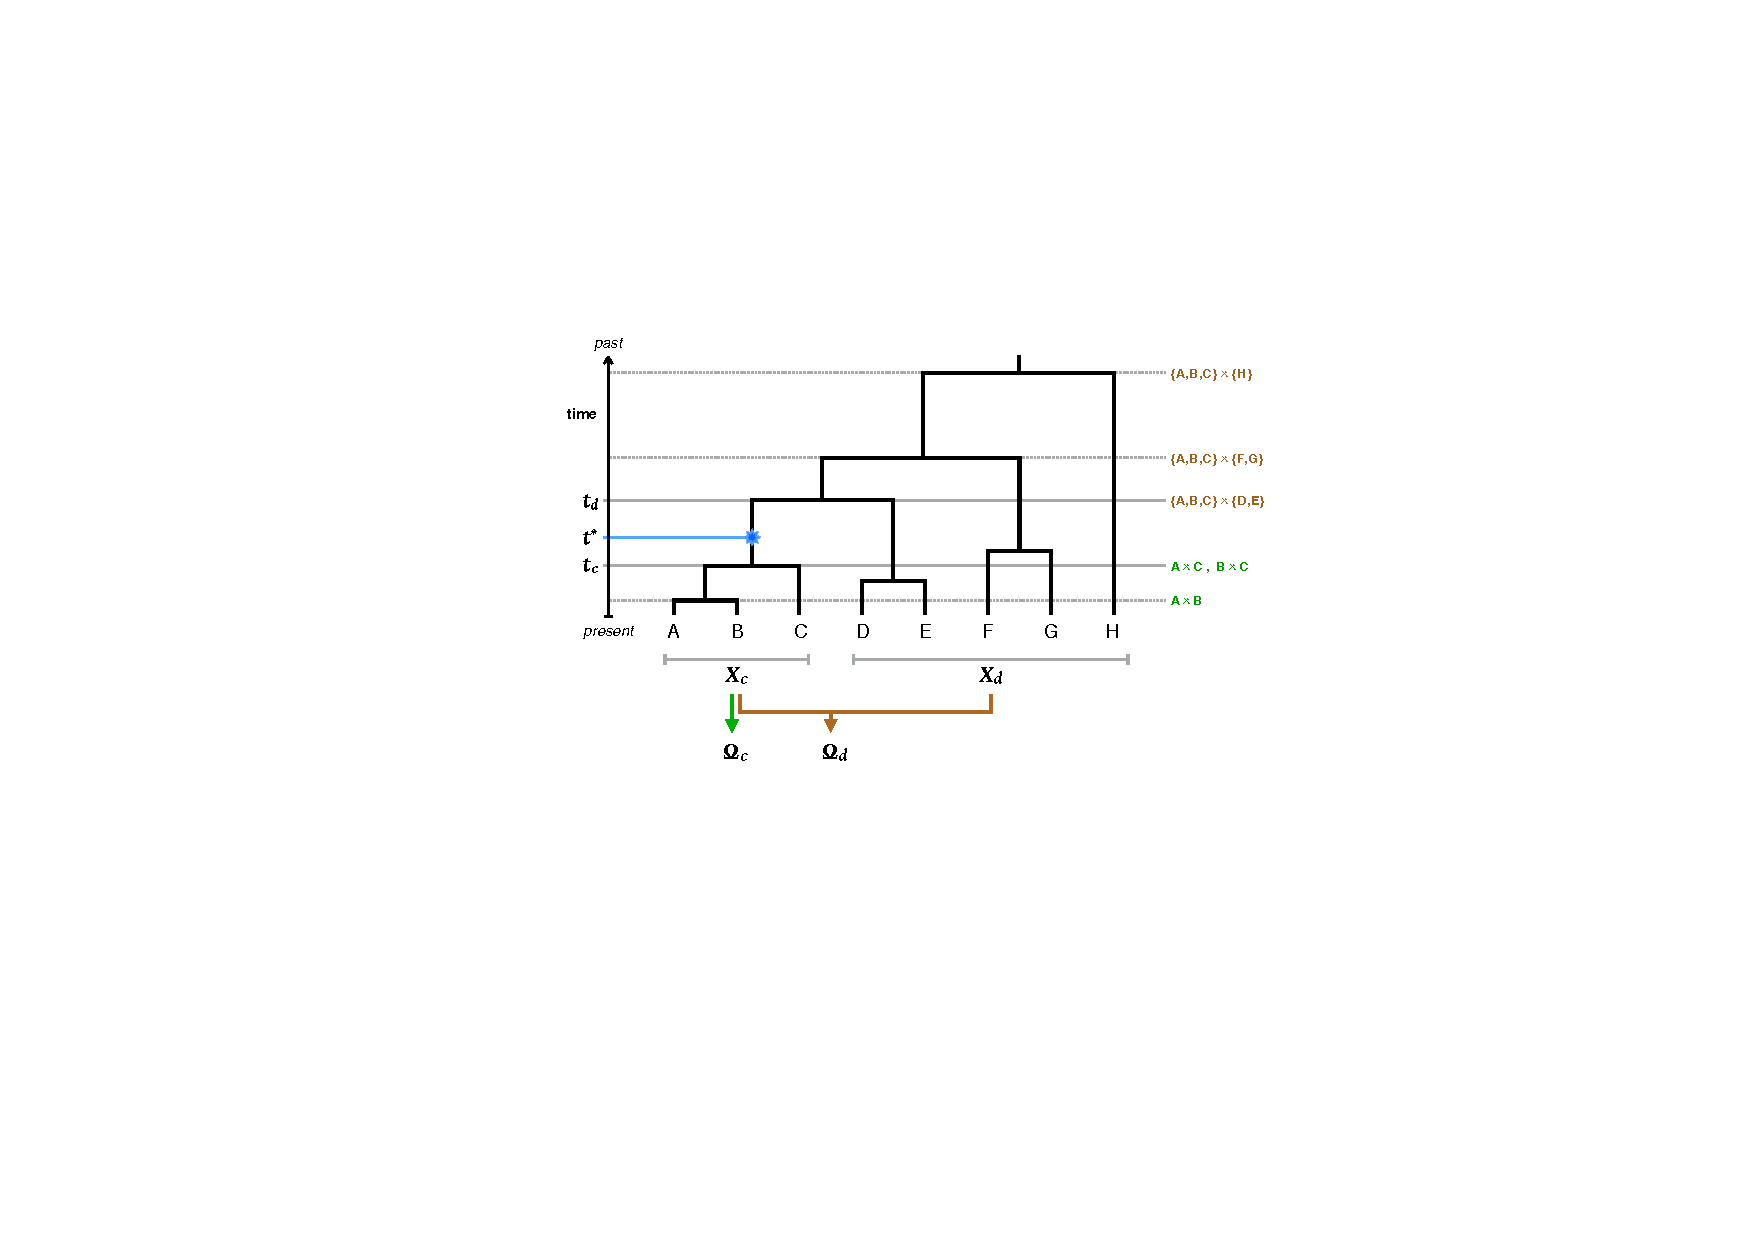
\includegraphics[width=\textwidth]{./img/ch5/info_age}
\Caption{Allele age in relation to concordant and discordant pairs}%
{The genealogy of a sample of \n{8} haplotypes is shown of which A, B, and C share a focal allele that derived from a mutation event as indicated in the tree (\emph{star}).
These chromosomes constitute the set of \emph{sharers}, denoted by $X_c$, which are differentiated from the set of \emph{non-sharers}, denoted by $X_d$.
Horizontal lines indicate the time of each coalescent event in the history of the sample within the local genealogy.
The time of the focal mutation event is denoted by ${t^\ast}$; the \n{2} coalescent events at time $t_c$ and $t_d$ define the length of the branch on which the focal mutation event occurred.
In particular, $t_c$ and $t_d$ correspond to the time until all haplotypes in $X_c$ have coalesced and the time at which the derived lineage joins the ancestral lineage of the most closely related haplotype in $X_d$, respectively.}%
{fig:info_age}
\end{figure}


% {\scriptsize \texthv{\textbf{(b)}}} \\
% \vspace{-30pt}
% \begin{center}
% \begin{tikzpicture}[-,auto,thick,
% txt/.style={font=\helvet\footnotesize,text width=4cm},
% lab/.style={font=\helvet\footnotesize,rectangle,draw=white,minimum size=0.2cm},
% sub/.style={circle,draw=white,fill=white,minimum size=0.7cm},
% con/.style={circle,draw=white,fill=oxgray!50,minimum size=0.6cm,outer sep=2pt,font=\helvet\footnotesize},
% dis/.style={circle,draw=white,fill=oxgray!50,minimum size=0.6cm,outer sep=2pt,font=\helvet\footnotesize}]
%
% \newcommand{\putConcordant}[2]{
% \node[sub] (dis#1) at (#2,1) {};
% \draw[-,draw=Brown!50,thick] (dis#1) to (conA);
% \draw[-,draw=Brown!50,thick] (dis#1) to (conB);
% \draw[-,draw=Brown!50,thick] (dis#1) to (conC);
% \node[con] (dis#1l) at (#2,1) {#1};
% }
%
% \node[txt] at (-0.5, 3.5) {$X_c$ (sharers)};
% \node[txt] at (-0.5, 1) {$X_d$ (non-sharers)};
%
%
% \node[lab,fill=ForestGreen!90] at (8, 3.775) {};
% \node[lab,fill=Brown!50] at (8, 3.275) {};
% \node[txt] at (10.25, 3.75) {Concordant pair $\in \Omega_c$};
% \node[txt] at (10.25, 3.25) {Discordant pair $\in \Omega_d$};
%
% \node[sub] (conA) at (2,3.5) {};
% \node[sub] (conB) at (4,3.5) {};
% \node[sub] (conC) at (6,3.5) {};
%
% \node[con] (conAl) at (2,3.5) {A};
% \node[con] (conBl) at (4,3.5) {B};
% \node[con] (conCl) at (6,3.5) {C};
%
% \draw [-,draw=ForestGreen!90,thick] (conA) to [out=18,in=162] (conB);
% \draw [-,draw=ForestGreen!90,thick] (conB) to [out=18,in=162] (conC);
% \draw [-,draw=ForestGreen!90,thick] (conC) to [out=144,in=36] (conA);
%
% \putConcordant{D}{1}
% \putConcordant{E}{2.5}
% \putConcordant{F}{4}
% \putConcordant{G}{5.5}
% \putConcordant{H}{7}
%
% \end{tikzpicture}
% \end{center}

%

It follows that all lineages in $X_c$ coalesce before any of them can coalesce with a lineage in $X_d$.
Any coalescent event between \n{2} lineages in $X_c$ must have occurred \emph{earlier} \Correct{than} the focal mutation event (back in time).
On the other hand, any coalescent event between \n{1} lineage in $X_c$ and \n{1} lineage in $X_d$ must have occurred \emph{later} than the focal mutation event (back in time).
Pairs of haplotypes in $X_c$ are referred to as \emph{concordant} pairs, whereas pairs formed by strictly taking one haplotype from $X_c$ and another from $X_d$ are \emph{discordant} pairs.
The sets $\Omega_c$ and $\Omega_d$ are defined to contain all concordant and discordant pairs, respectively.

\Correct{In the following, I describe how the posterior density of the \gls{tmrca} is obtained for concordant and discordant pairs to eventually arrive at an estimate of allele age.
To distinguish the population-scaled time $\tau$, as defined for the \gls{tmrca}, from the time of the mutation event, let the latter be denoted by the likewise population-scaled time $t$.}
\Correct{Informally, the actual time of a mutation event} is found at the ``sweet~spot'' in between the earlier coalescent event at time $t_c$ and the later coalescent event at time $t_d$; see \cref{fig:info_age}.

% Posteriors are obtained for concordant pairs in $\Omega_c$ where the \emph{oldest} relation may indicate the lower bound in the estimation of the focal allele age.
% Likewise, posteriors are obtained for discordant pairs in $\Omega_d$ where the \emph{youngest} relation indicates the upper bound.


%
\subsubsection{Cumulative coalescent function (CCF)}\label{sec:ccf_desc}
%

\CorrectNote{Section partially rewritten with revised notation}

At a given focal site at which the possible concordant and discordant pairs in the sample have been sorted into the sets $\Omega_c$ and $\Omega_d$, respectively, each pair is analysed in turn to obtain a posterior on their \gls{tmrca}.
Importantly, to find the time of the focal mutation event, it is of interest to obtain the probability distribution of the \gls{tmrca} relative to $t$.
Here, this task is accomplished by introducing the \gls{ccf} which is defined as the posterior \gls{cdf} with respect to a given pair of haplotypes, denoted by ${i,j}$.
In simple terms, the \gls{ccf} is expressed as
\begin{equation}\label{eq:cumcoalfunc}
	\Phi_{ij}(t)~=~
	\begin{cases}
    ~ P(\tau \leq t)                  & \text{if}~{\{i,j\} \subseteq \Omega_c}\quad\text{(\ie concordant pairs)} \\
    ~ P(\tau >    t)=1-P(\tau \leq t) & \text{if}~{\{i,j\} \subseteq \Omega_d}\quad\text{(\ie discordant pairs)}\text{.}
  \end{cases}
\end{equation}
Specifically, the term ${P(\tau \leq t)}$ implies that concordant pairs have coalesced \emph{earlier} than or at the time of the focal mutation event (back in time), and ${P(\tau >t)}$ implies that discordant pairs have coalesced \emph{later} than the mutation event (back in time).

Since each clock model defines the posterior using the Gamma distribution, it is straightforward to obtain the \gls{ccf} from the Gamma~\gls{cdf}; formally given as
\begin{equation}
	G(t)~=~P(\tau \leq t \mid\alpha,\beta)~=~\int_{0}^{t}g(u\mid\alpha,\beta)~du
\end{equation}
where $\alpha,\beta$ are defined according to the clock model used, with parameter values obtained from the analysis of a given haplotype pair at a focal site in the genome.
Notably, because $\alpha$ is a positive integer in each of the clock models considered, the Gamma distribution simplifies to the Erlang distribution, such that the above becomes equal to \citep{papoulis2002probability}
\begin{equation}
	F(t)~=~P(\tau \leq t \mid\alpha,\beta)~=~1-\euler{-\beta t}\sum_{i=0}^{\alpha-1}\frac{(\beta t)^i}{i!}\text{.}
\end{equation}

Further, to obtain point estimates from the posterior of the \gls{tmrca},
it follows from the Gamma (Erlang) distribution that the mean is $\frac{\alpha}{\beta}$ and the mode is $\frac{\alpha-1}{\beta}$.
Note that no simple closed form exists for the median, but which in practise is straightforward to approximate by scanning the \gls{ccf} to find, for example, the times of the \nth{1}, \nth{2} (\ie median), and \nth{3} quartiles.


% Each clock model described above computes the posterior probability for \n{2} lineages to have coalesced at a particular point in time.
% This is extended such that the posterior distribution of coalescent times is calculated over a continuous time prior such that the \gls{tmrca} can be derived from the \gls{cdf}.
% Here, this approach is referred to as the \gls{ccf} which is defined as
%
% where $t$ denotes the coalescent time prior and $i,j$ denote the \n{2} haplotypes under consideration.
% The parameterisation of the clock model used is indicated by ``$\cdot$''.
% In practise, the posterior probability ${p(\tau\mid\cdot)}$ is calculated from the Gamma (Erlang) distribution in each clock model, due to the conjugate relation described in the previous section.


%
\subsubsection{Allele age estimation from the composite posterior distribution}\label{sec:comp_post_detail}
%

\CorrectNote{Section partially rewritten with revised notation}

A at given focal site, the \gls{ccf} is obtained for concordant and discordant pairs.
Because the \gls{tmrca} of concordant pairs would extend to a point below the focal mutation event and the \gls{tmrca} of discordant pairs above that point in time, ideally, it would be expected that the age of an allele can be derived from the structure of posteriors.
Here, the \gls{ccf} posteriors are combined in the following way.
\begin{equation}\label{eq:comp_post}
	\Lambda_k(t)~\propto~\prod_{i,j \in A_k} \Phi_{ij}(t\mid\alpha,\beta)
\end{equation}
for focal site $k$ at which haplotype pairs have been sorted into the collection ${A_k=\{\Omega_c,\Omega_d\}}$, according to allele sharing at that site.
Again, ${\alpha,\beta}$ are defined by the clock model used and obtained from parameter values observed for pair ${i,j}$.
In the following, the term \emph{composite posterior} is used to refer to the result obtained using \cref{eq:comp_post}.

%
%!TEX root = ../../main.tex


\begin{figure}[!htb]
\centering
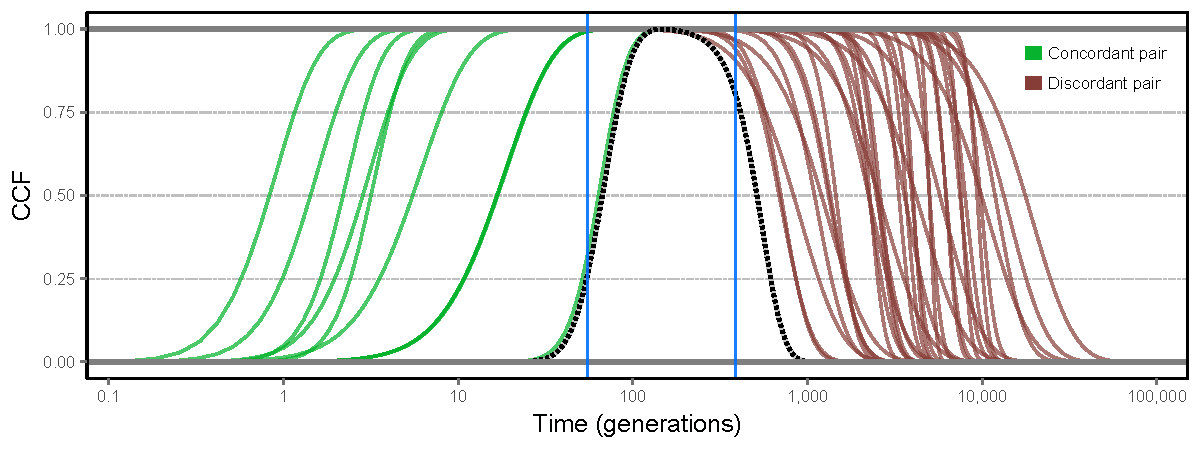
\includegraphics[width=\textwidth]{./img/ch5/age_example_new}
\Caption{Example of concordant and discordant posterior distributions and the resulting composite posterior}%
{A target variant was randomly selected from simulated data.
The \gls{ccf} was obtained for the set of possible concordant pairs and a subset of concordant pairs, which were randomly selected.
The thicker \emph{dotted} line shows the distribution of the maximised composite posterior.
The \emph{blue} lines mark the times of coalescent events below and above the focal mutation event; \ie $t_c$ (\emph{left}) and $t_d$ (\emph{right}), determined from simulation records.
Their distance corresponds to the length of the branch on which the focal mutation event occurred.}%
{fig:age_example}
\end{figure}

%

The composite posterior distribution can now be obtained over ${t \in (0,\infty)}$.
However, in practise, it is unlikely that the relationship of ${i,j}$ can be traced back further than a small multiple of \Ne (\eg $\sim 10$).
An example is given in \cpref{fig:age_example}, showing the \gls{ccf} for concordant and discordant pairs, as well as the maximised composite posterior distribution.
Notably, the ``width'' of the distribution is expected to be determined by the underlying branch length.
In the following, the mode of the composite posterior distribution is taken as a point estimate for the age of an allele, denoted by $\hat{t}$.



% The lower and upper bounds on the estimated age are provided by the incomplete gamma functions
% \begin{equation}
% 	P_{i,j}(\tau > t) ~=~ \int_{0}^{\tau} \Phi(t \mid i,j) ~dt
% \end{equation}
% and
% \begin{equation}
% 	P_{i,j}(\tau < t) ~=~ \int_{\tau}^{\infty} \Phi(t \mid i,j) ~dt \ .
% \end{equation}
%
% The composite likelihood estimate of the time is scaled in units of ${2 \Ne}$.
% The mean, median, and mode of the posterior distribution were taken as age estimates.
% In the following, the estimated age is reported using the median, which is denoted by $\hat{t}$ and expressed in units of generations.
% The example shown in \cpref{fig:age_example} illustrates the output produced for a single focal variant.



%
\subsubsection{Note on composite likelihood methods}
%

\AdditionNote{Section included}

There is extensive literature on the topic of composite likelihood methods and their application to problems where the full likelihood function cannot be known or is intractable.
In its general form, the composite likelihood is defined as the weighted product of the likelihoods associated with a set of events ${\{X_1,\ldots,X_z\}}$; \ie \citep{lindsay1988composite}
\begin{equation}\label{eq:simple_cl}
	\mathcal{C\!L}(\vartheta\mid y)~=~\prod_{z\in Z} \mathcal{L}_z(\vartheta\mid y)^{w_z}
\end{equation}
where ${\mathcal{L}_z(\vartheta\mid y)}$ is the likelihood function proportional to density ${f(y\in X_z \mid \vartheta)}$ with parameter (vector) $\vartheta$, and $w_z$ are non-negative weights.

The use of the composite likelihood in a Bayesian setting has been discussed, for example, by \citet{pauli2011bayesian} who argued that, formally, a posterior distribution can be obtained with the composite likelihood; \ie
\begin{equation}
	p_{\mathcal{C\!L}}(\vartheta\mid y)~\propto~\pi(\vartheta)~\times~\mathcal{C\!L}(\vartheta\mid y)
\end{equation}
where ${\pi(\vartheta)}$ is a suitable prior on the parameter.
The properties of the above were described by \citet{pauli2011bayesian} who, as a result, proposed an adjustment to the composite likelihood by choosing appropriate weights ($w_z$) to improve approximation of the full posterior distribution.

The ``composite posterior'' given in \ctref{eq:comp_post} follows a similar approach in context of the above, but is defined proportional to the product of posteriors.
While ${\Lambda_k(t)}$ itself cannot be regarded as a composite likelihood, it can be argued that the proposed method is an (\emph{ad hoc}) approach equivalent to using the composite likelihood in a Bayesian setting, yet without specifying an appropriate weighting function.



%
\subsubsection{Note on the computational burden}
%

A major caveat is the computationally demanding analysis of each haplotype pair in $\Omega_c$ and $\Omega_d$ per target site.
The number of concordant and discordant pairs, denoted by $n_c$ and $n_d$, respectively, varies dependent on the observed frequency of the focal allele and sample size.
For a given \fk{}~variant, the number of possible concordant pairs is
\begin{equation}\label{eq:age_nc}
	\max[n_c] ~=~ {{k}\choose{2}} ~=~ \frac{k(k-1)}{2}
\end{equation}
where $k$ is the number of allele copies observed in the sample.
The number of possible discordant pairs is given by
\begin{equation}\label{eq:age_nd}
	\max[n_d] ~=~ k(2N-k)
\end{equation}
where $N$ refers to the diploid sample size.
The total number of pairwise analyses conducted per target site is the sum of $n_c$ and $n_d$.

The estimation process for a single focal allele quickly becomes intractable if the allele is observed at higher frequencies or if sample size is large.
This can be particularly problematic if many target sites are considered.
For example, for ${N=\num{1000}}$, each \fk{2}~variant has ${n_c=2}$ and ${n_d=\num{3996}}$, whereas each \fk{20}~variant already has ${n_c=\num{190}}$ and ${n_d=\num{19600}}$.
Therefore, in practise, the computational burden is reduced by employing a sampling regime where, for example, pairs in $\Omega_c$ and $\Omega_d$ are picked at random.

% To make the age estimation analysis computationally tractable, a sampling regime was employed which randomly pairs individual chromosomes drawn from $X_c$ and $X_d$ until a nominal threshold of unique pairs in $\Omega_c$ and $\Omega_d$ is reached.
% Note that the \texttt{rvage} algorithm in its current implementation includes all possible concordant pairs in $\Omega_c$, because ${\max[n_c]}$ is assumed to be reasonably small if the focal allele frequency is low, even in larger samples of thousands of individuals.
% Hence, the method specifies a sampling threshold as the upper limit of $n_d$.


\DeleteNote{Section ``Anticipated limitations''}

%
% %
% \subsubsection{Anticipated limitations}
% %
%
% Since the estimation of allele age is dependent on parameters inferred from the underlying IBD structure of the sample, the accuracy of IBD detection is expected to affect the accuracy of the estimated age.
% %
% %!TEX root = ../../main.tex


\begin{figure}[p]
\centering
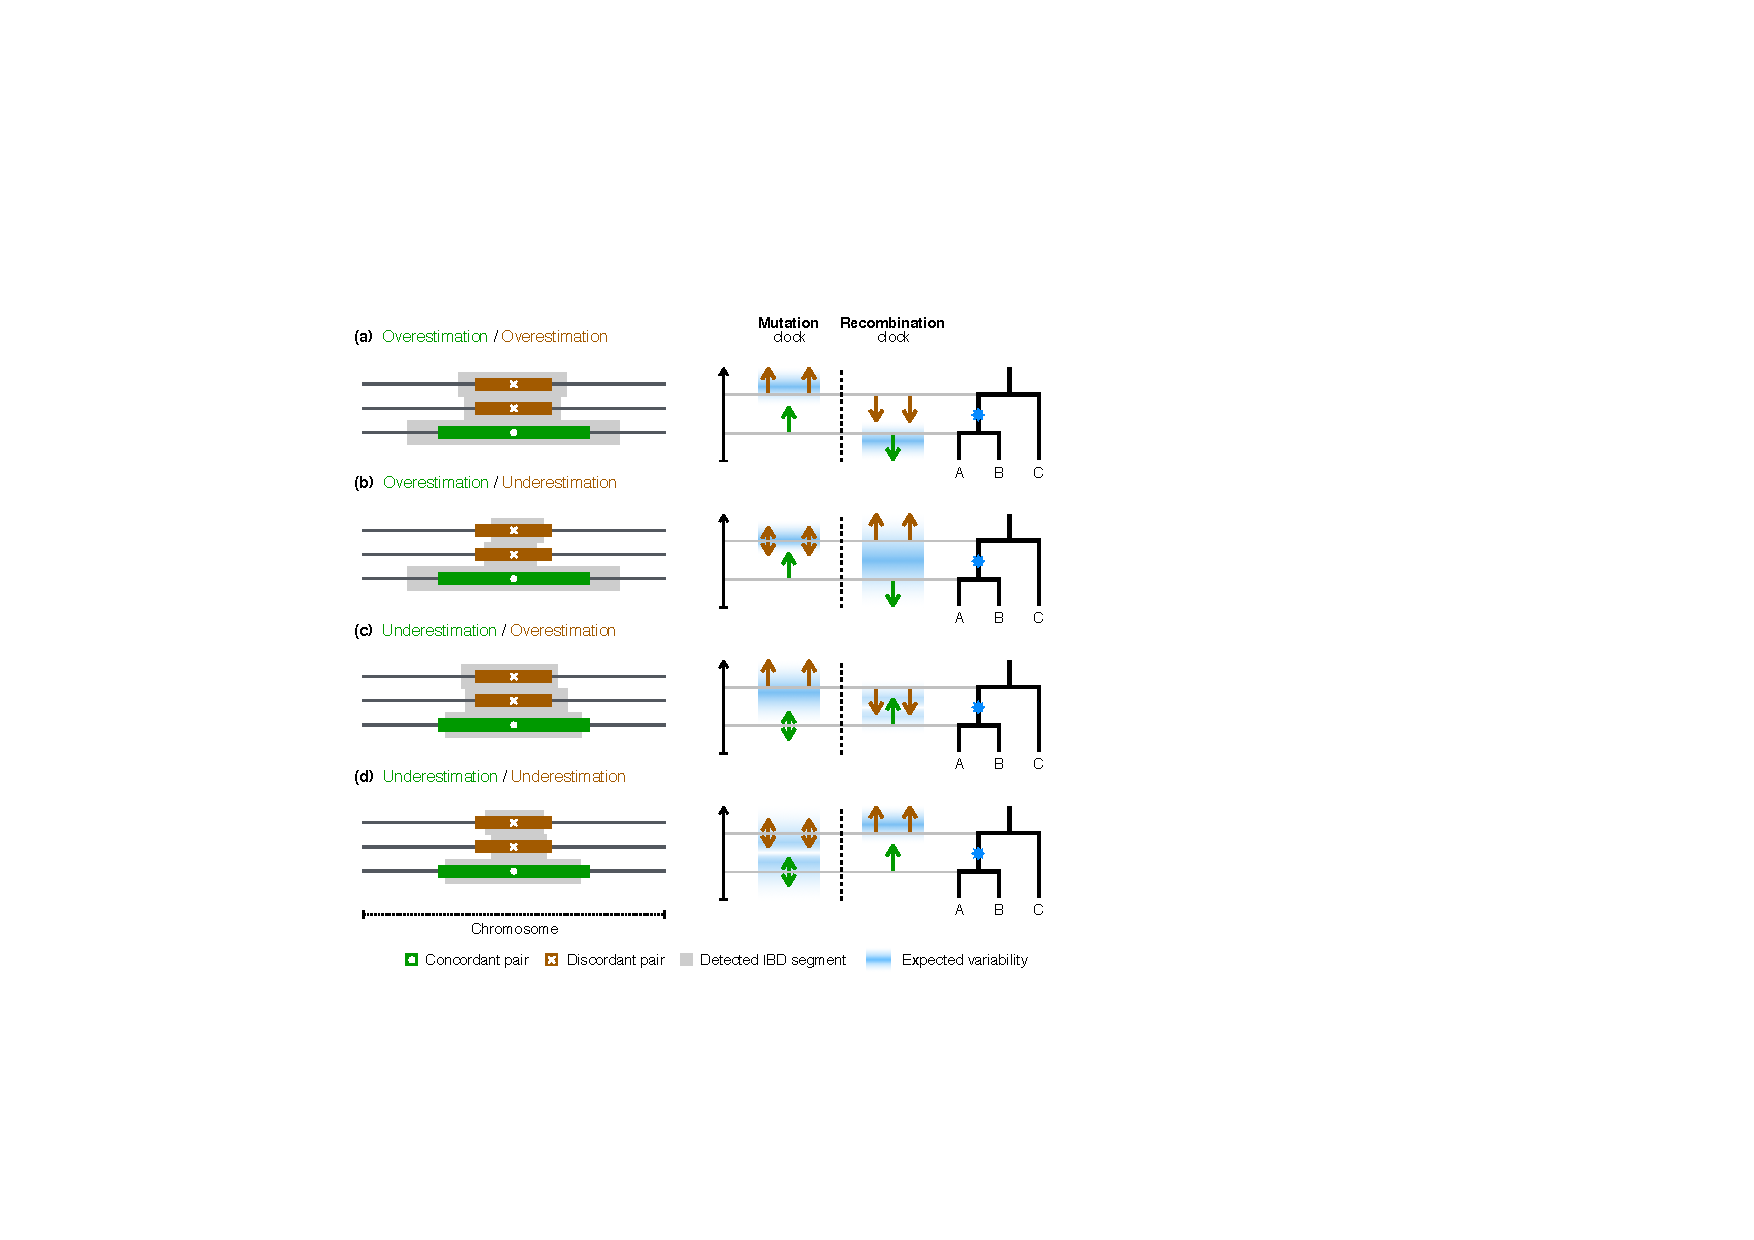
\includegraphics[width=\textwidth]{./img/ch5/info_age_bias}
\Caption{Expected estimation bias due to deficient IBD inference}%
{A minimal example is illustrated for a sample of \n{3} chromosomes where ${A,B \in X_c}$ and ${C \in X_d}$.
The focal mutation event is indicated in the genealogy of the sample (\emph{star}).
Each pair shares some haplotype region identical by decent, where the actual extent of the underlying IBD segment is shown for the concordant pair ${\{A,B\}}$ and the discordant pairs ${\{A,C\}}$ and ${\{B,C\}}$; indicated by \emph{green} and \emph{brown} bars, respectively.
The allele shared in concordant pairs is indicated (\emph{circle}), as well as the absence of allele sharing in discordant pairs (\emph{cross}).
Inferred IBD segments are shown as \emph{grey} bars at each true IBD segment, which may overestimate or underestimate the actual shared haplotype length.
Panels~\textbf{(a)} to \textbf{(d)} illustrate the possible cases of over and underestimation when observed in concordant and discordant pairs.
The arrows shown in relation to the times of coalescent events in the genealogy indicate the  direction to which the estimation under a given clock model is expected to tend, given the respective pattern of over and underestimation in concordant and discordant pairs.
The expected variability of the estimated age posterior distribution is indicated (\emph{blue}).
Note that only the mutation clock, \ClockM, and the recombination clock, \ClockR, are shown because \ClockC is a combination of both models.}%
{fig:info_age_bias}
\end{figure}
%
% %
% Possible consequences of inaccurately inferred lengths of IBD segments are summarised in \cpref{fig:info_age_bias}, which illustrates a minimal example for the different cases possible when concordant or discordant IBD length is over or underestimated.
% For instance, in cases where IBD is overestimated in both concordant and discordant pairs (\cref{fig:info_age_bias}{a}), both the the genetic length and the number of pairwise differences, $S$, may be inflated, which affects the computation of the \gls{ccf} under the mutation and recombination clock differently.
% Notably, because the pairwise probability distributions computed by the \gls{ccf} in the set of pairs are multiplied to calculate the composite likelihood in \cref{eq:compll}, it is possible that some analyses my return invalid results, as probabilities may cancel out or become too small to be distinguishable from zero given machine limits.
% In the following, the term \emph{conflict} is used to refer to sites at which the analysis returned an invalid age estimate.
%










%
\section{Evaluation}
%


\Correct{The following sections describe the data used in this chapter, as well as the metrics used to evaluate age estimation results.}



%
\subsection{Data generation}
%

\Correct{The following simulated datasets were available.}
First, sample data were simulated under a simple demographic model of constant population size (${\Ne = \num{10000}}$) with mutation rate ${\mu=\num[round-precision=1]{1e-08}}$ per site per generation and constant recombination rate ${\rho=\num[round-precision=1]{1e-08}}$ per site per generation, using \texttt{msprime} \citep{Kelleher:2016fn}.
Note that by setting the mutation and recombination rates to constant and equal values, the physical and genetic lengths are identical when measured in \gls{Mb} and \gls{cM}, respectively.
The size of the simulated dataset was \n{2000} haplotypes, which were randomly paired to form a sample of ${N=\num{1000}}$ diploid individuals.
The length of the simulated region was \SI{100}{\mega\basepair} (\SI{100}{\centi\morgan}), resulting in \n{326335}~variant sites.
This dataset is denoted by $\mathcal{D}_A$.

Second, the dataset simulated in Chapter~3 was included here to evaluate the age estimation method in presence of data error.
Briefly, the simulation was performed under a demographic model that recapitulates the human expansion out of Africa; following \citet{Gutenkunst:2009gs}.
A sample of \n{5000} haplotypes was simulated with ${\Ne=\num{7300}}$, a mutation rate of ${\mu=\num[round-precision=2]{2.35e-8}}$ per site per generation, and variable recombination rates taken from human chromosome~20; Build~37 of the \gls{hapmap} Phase~\rom{2} \citep{Frazer:2007kha, InternationalHapMapConsortium:2010en}, yielding \dec{0.672847}~million segregating sites over a chromosomal length of \SI{62.949301}{\mega\basepair} (\SI{108.26675653}{\centi\morgan}).
The simulated haplotypes were randomly paired to form a sample of ${N=\num{2500}}$ diploid individuals.
Haplotype data were converted into genotypes and subsequently phased using \texttt{SHAPEIT\,2} \citep{Delaneau:2008dk,Delaneau:2013hi}.
This facilitated the assessment of the impact of phasing error on the age estimation process.

Third, the dataset described above was retrofitted in Chapter~4 to include realistic proportions of empirically estimated error, which was equally distributed in the derived genotype and haplotype datasets \Correct{(both ``true'' and phased haplotype data)}.
Here, data \emph{before} and \emph{after} the inclusion of error are distinguished by referring to dataset $\mathcal{D}_B$ and dataset $\mathcal{D}_B^{\ast}$, respectively.
Note that in the following the term \emph{genotype error} is used, even in analyses that operate on haplotype data, as error proportions were estimated from misclassified genotypes \Correct{in \gls{1kg} data (``1000G.A'' in Chapter~4, \ccref{sec:err_test_data}).}


In each dataset, simulation records were queried to determine the underlying IBD structure of each pair of individuals analysed in this work.
Note that the simulated genealogy underlying $\mathcal{D}_B$ was identical to $\mathcal{D}_B^{\ast}$, such that direct comparisons were possible between results obtained before and after error.
True IBD intervals were found in simulated genealogies by scanning the sequence until the \gls{mrca} of a given pair of haplotypes changed, on both sides of a given target position.
Interval breakpoints were identified on basis of the observed variant sites in the sample, such that the resulting true IBD segment defined the smallest interval detectable from available data.

% Note that this allowed overestimation of the actual genetic length of the IBD segment, but thereby provided a realistic benchmark for comparisons with IBD detection methods; namely the \gls{fgt}, \gls{dgt}, and the \gls{hmm}-based approach as implemented in the \texttt{rvage} algorithm.



%
\subsection{Accuracy analysis}
%

Coalescent simulators may not define the exact time point at which a mutation event occurred, because mutations are independent of the genealogical process (if simulated under neutrality) and can therefore be placed randomly along the branches of the simulated tree.
Mutation times are not specified in \texttt{msprime}, but the times of coalescent events are recorded.

In simulations, the probability of placing a mutation on a particular branch is directly proportional to its length, which itself is delimited by the time of the coalescent event below (joining the lineages that derive from that branch) and the time of the coalescent event above (joining that branch with the tree back in time).
Here, the times of coalescence below and above a particular mutation event are denoted by $t_c$ and $t_d$, respectively, against which the accuracy of the estimated allele age $\hat{t}$ is measured.

Although the true time of a mutation event was not known from the simulations performed, an indicative value for the age of an allele was derived from the logarithmic ``midpoint'' (or \emph{log-average}) between coalescent events, which is denoted by $t_m$ and calculated as the geometric mean of $t_c$ and $t_d$, namely
\begin{equation}
	t_m~=~\sqrt{~t_c ~ t_d~}\text{.}\CorrectLabel
\end{equation}
\Correct{However, note that the arithmetic mean, ${\frac{1}{2}(t_c + t_d)}$, would be appropriate given that mutation events can be placed uniformly between $t_c$ and $t_d$.
The geometric mean is nonetheless useful and was chosen for practical reasons (\eg representation on log-scale).}

% \begin{equation}
% 	t_m ~=~
% 	\exp \bigg[ \log \big[ t_c \big] + \frac{1}{2} \bigg( \log \big[ t_d \big] - \log \big[t_c \big] \bigg) \bigg] ~=~
% 	\sqrt{~t_c ~ t_d~}
% \end{equation}

Accuracy was measured using Spearman's rank correlation coefficient, $r_S$, which is a robust measure for the strength of the monotonic relationship between \n{2} variables; \ie the inferred allele age ($\hat{t}$) and true time proxies ($t_c$, $t_m$, or $t_d$).
Note that the squared Pearson correlation coefficient, $r^2$, was used in previous chapters but \Correct{was regarded as being} less suitable here, as both the inferred and true age are expected to vary on log-scale, and the Pearson coefficient measures the linear relationship between variables.
\Correct{However, for example, $r^2$ of log-transformed age could have been used, but which was not additionally considered here, in order to keep the analysis brief.}
Also, \Correct{to indicate bias}, the \gls{rmsle} was calculated as a descriptive score for the magnitude of error (here defined on $\log_{10}$).

To better illustrate the distribution of age estimates obtained in an analysis, the \emph{relative age} was computed, $\hat{t}_\textit{rel}$, for each allele by normalising the time scale conditional on the time interval between the coalescent events at $t_c$ and $t_d$, such that age estimates were ``mapped'' on the same scale relative to the branch length spanned between $t_c$ and $t_d$; this was calculated as below.
\begin{equation}\label{eq:age_relative}
	\hat{t}_\textit{rel} ~=~
	\frac{ \log \big[ \frac{\hat{t}}{t_c} \big] }{ \log \big[ \frac{t_d}{t_c} \big] }
\end{equation}
As a result, the times of coalescent events at $t_c$ and $t_d$ are mapped to 0 and 1, respectively.
It follows that that ${\hat{t}_\textit{rel} < 0}$ indicates underestimation and ${\hat{t}_\textit{rel} > 1}$ overestimation in relation to the true interval in which the mutation event could have occurred.

Further, an age estimate was counted as being ``correct'' if ${t_c \leq \hat{t} \leq t_d}$, which is equal to the condition ${0 \leq \hat{t}_\textit{rel} \leq 1}$.
The proportion of age estimates that fall within this interval is reported.











%
\section{Validation of the method}\label{sec:age_validation_analysis}
%


The allele age estimation method relies on \Correct{an (ideally) correct} inference of the haplotype region shared by descent between \n{2} chromosomes relative to a target site.
\Correct{Several approaches for targeted, pairwise inference of the shared haplotype have been developed in the previous chapters, which are applied further below.
To first establish \emph{proof of concept} of the age estimation method, its performance was evaluated given complete knowledge of the underlying shared haplotype structure.
That is, the ``true'' shared haplotype segments were determined from simulation records and analysed using haplotype data in dataset $\mathcal{D}_A$.}

\Correct{Further,} because an exhaustive analysis of all possible haplotype pairs becomes computationally intractable, it is convenient to reduce the number of pairwise analyses that are conducted per target allele.
% For example, although the sample size of dataset $\mathcal{D}_A$ was modest (${N = \num{1000}}$), the total number of possible pairwise analyses for the set of \n{10000} selected rare variants would have been \dec{145.724783}~million.
%For realistic applications of the method, it is therefore essential to reduce the number of pairs.
\Correct{In particular, because the current analysis focused on rare alleles,} the number of discordant pairs, $n_d$, was reduced such that ${\Omega_d}$ consisted of a substantially smaller set of randomly retained pairs.
Here, the impact on estimation accuracy was assessed under different nominal thresholds applied to $n_d$ (listed below).
% Importantly, to focus on the impact resulting from different $n_d$ thresholds, the analysis was conducted using true IBD segments as determined from simulation records.
% Thus, this section provides a general validation analysis of the age estimation method.

\begin{center}
\begin{tabular}{r@{\hskip 2em}r}
{$n_d$} &
{Pairwise analyses} \\
	\midrule
	\num{10}   & \dec{0.461842} million \\
	\num{50}   & \dec{0.861842} million \\
	\num{100}  & \dec{1.361842} million \\
	\num{500}  & \dec{5.361842} million \\
	\num{1000} & \dec{10.366135} million \\
\end{tabular}
\end{center}

A number of \n{10000}~rare variants were randomly selected as target sites at allele frequency~${\leq \SI{1}{\percent}}$ (\fk{[2,20]}).
Each clock model was considered separately and the same set of sites was analysed under each threshold.
However, note that because discordant pairs were chosen at random, these differed in each analysis.
%This resulted in a total of \dec{276.1326}~million pairwise analyses in this section alone.
% None of the analyses returned conflicting results; recall that \emph{conflicts} were defined as invalid estimates resulting from erroneous patterns of coalescent times as computed through the \gls{ccf} for the set of pairs considered.
%Note that discordant pairs were formed randomly and therefore differed in each analysis.
Model parameters in \texttt{rvage} were specified according to parameters used for the simulation of $\mathcal{D}_A$ (${\Ne=\num{10000}}$; ${\mu=\num[round-precision=1]{1e-08}}$; ${\rho=\num[round-precision=1]{1e-08}}$).


%
\subsection{Results}
%


An overview is illustrated in \cpref{fig:discords_scat}, which shows the density of true and estimated age under each clock model; results are shown for ${n_d=\num{10}}$, ${n_d=\num{100}}$, and ${n_d=\num{1000}}$, to better distinguish differences visually.
\Correct{Note that, here, true age was set to $t_m$ (the geometric mean of $t_c$ and $t_d$).}


%
% !TEX root = ../../main.tex


\begin{figure}[p]
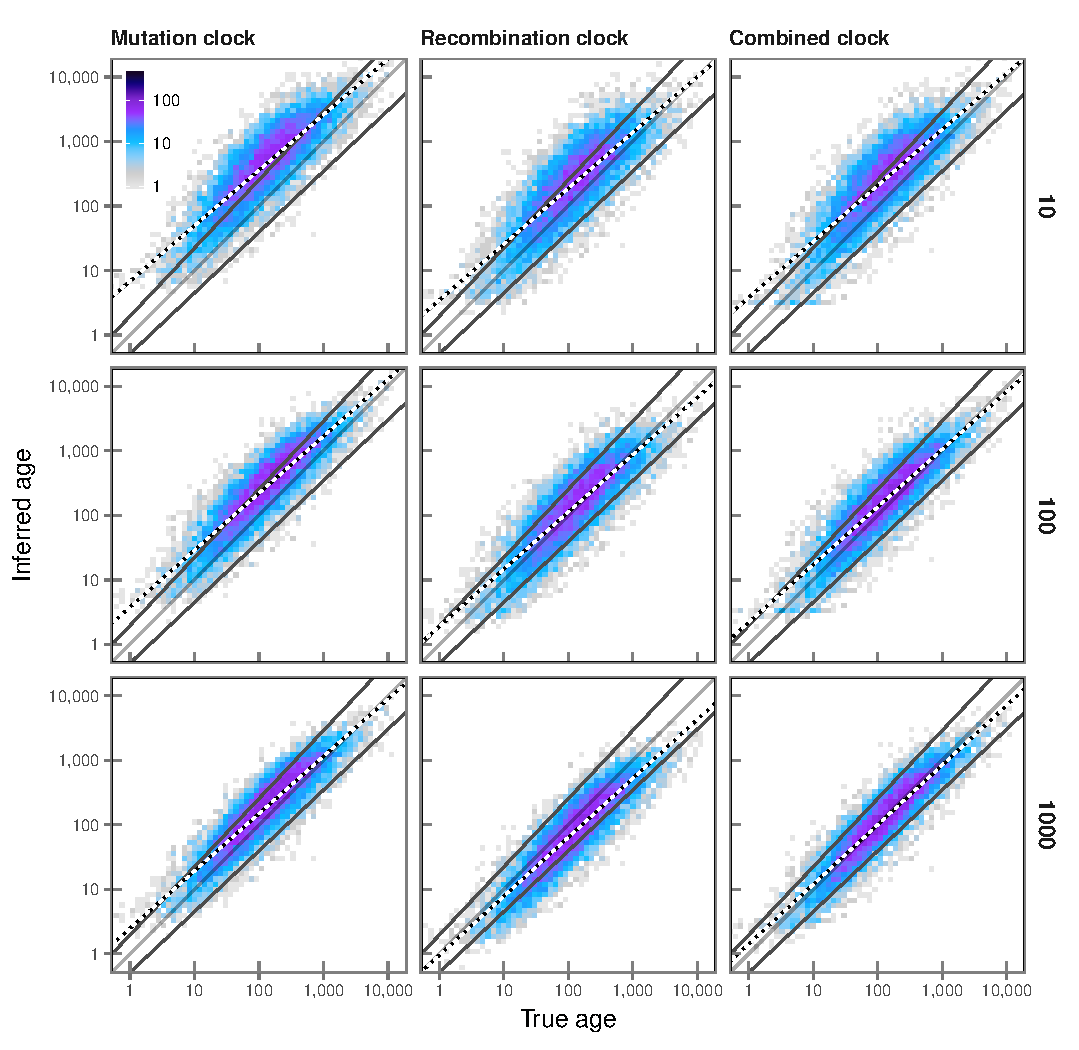
\includegraphics[width=\textwidth]{./img/ch5/discords_scat}
\Caption{True and inferred age under varying numbers of discordant pairs}
{A set of \n{10000} target sites was randomly drawn in \fk{[2,20]} (shared allele frequency ${\leq 1\%}$) in a simulated sample of \n{2000}~haplotypes.
Different numbers of sampled discordant pairs were analysed on the same set of target variants, which is shown for ${n_d = \num{10}}$, ${n_d = \num{100}}$, and ${n_d = \num{1000}}$ (indicated at the \emph{right} of each row).
True IBD was used to estimate allele age.
IBD breakpoints were determined from simulation records and defined as the first variant sites observed in the data following the \n{2} recombination events on each side of a given focal position.
Age was estimated under each of the \n{3} clock models; \ie mutation clock, \ClockM, recombination clock, \ClockR, and combined clock, \ClockC (indicated at the \emph{top} of each column).
Each panel shows the density distribution of true and inferred age (numbers indicated by the colour-gradient).
Note that the ``true age'' of a focal allele was set to $t_m$, which is the geometric mean of $t_c$ and $t_d$, \ie the true time of the coalescent event from which the focal allele derived ($t_c$) and the true time of the coalescent event immediately preceding that event ($t_d$) in the history of the sample, respectively; these are indicated by their regression trend lines \emph{below} and \emph{above} the dividing line at $t_m$, respectively.
The \emph{black-white} line indicates the line of best fit resulting from linear regression of age estimates, using the posterior mode of the composite likelihood distribution as the inferred age value.
True and inferred age are both shown on log-scale.}
{fig:discords_scat}
\end{figure}

%

Despite the substantial difference in the number of pairwise analyses, overall accuracy was high for each threshold and under each clock model.
A higher $n_d$ threshold was generally found to improve overall accuracy.
At lower thresholds, each model showed a tendency to overestimate allele age, which most likely resulted from the smaller set of discordant pairs, as the individuals that are more closely related to the focal haplotypes may or may not be captured.

% Interestingly, the recombination clock, \ClockR, showed a tendency to underestimate allele age at higher thresholds, despite using true IBD segments.
% This observation may be the result of an overestimation of true IBD lengths, since IBD breakpoints were determined from the set of variant sites observed in the data.
% Note that allele age is generally expected to be underestimated if genetic lengths in concordant or discordant pairs are overestimated, as a longer IBD segment is indicative for more recent haplotype sharing (\ie recombination had less time the break down the length of a shared haplotype).
% The average distance between consecutive variant sites in ${\mathcal{D}_A}$ was \SI{3.064307e-04}{\centi\morgan} (\dec{306.4307} basepairs), showing that even small inaccuracies in IBD can affect the estimation of allele age (under the recombination clock).

The proportion of target alleles for which age was correctly estimated \Correct{(${t_c \leq \hat{t} \leq t_d}$)} increased with higher $n_d$ thresholds under each clock model.
This was lowest in \ClockM, where \SIlist{36.61;51.11;66.28}{\percent} were correctly inferred for $n_d$ at \numlist{10;100;1000}, respectively, and relatively high in \ClockR, where \SIlist{55.79;70.60;70.51}{\percent} were correct, respectively.
The highest proportion of correct alleles was \SI{79.93}{\percent} in \ClockC and ${n_d = \num{1000}}$.
The proportion of overestimated alleles (${\hat{t} > t_d}$) decreased in all clock models at higher $n_d$ thresholds, showing a modest decrease in \ClockM (\SIrange{63.38}{32.66}{\percent} for $n_d$ at \num{10} and \num{1000}, respectively), a substantial decrease in \ClockR (\SIrange{43.45}{6.45}{\percent}, respectively), and a notable decrease in \ClockC (\SIrange{46.78}{15.64}{\percent}, respectively).
Since \ClockM showed a tendency to overestimate allele age, the proportion of underestimated alleles was low (\SI{1.06}{\percent} for ${n_d = \num{1000}}$), which was similarly low in \ClockC (\SI{4.43}{\percent}), and highest in \ClockR (\SI{23.04}{\percent}).

%
% !TEX root = ../../main.tex


\begin{table}[!htb]
\Caption{Estimation accuracy under varying numbers of discordant pairs}
{Different thresholds for the number of randomly formed discordant pairs, $n_d$, were analysed to evaluate the impact on the accuracy of allele age estimation.
Note that all possible concordant pairs were included in each analysis; \ie $n_c$ was not reduced.
True IBD segments were used to focus on the differences induced by varying $n_d$ thresholds.
Each analysis was conducted on the same set of \n{10000} randomly selected rare variants at allele frequency ${\leq 1\%}$.
Accuracy was measured using the rank correlation coefficient, $r_S$, and the magnitude of error, \gls{rmsle}, between the estimated age, $\hat{t}$ and the times of coalescent events; \ie the time until all haplotypes in $X_c$ have coalesced, $t_c$, and the time of the immediately preceding coalescent event, $t_d$, which joined the lineages in $X_c$ and $X_d$ back in time, as well as the geometric mean of both, $t_m$.}
{tab:stats_discords}
\centering
\begin{tabular}{cS[table-format=4.0]*6{S[table-format=1.3]}}
\toprule
Clock & {$n_d$} &
\multicolumn{3}{c}{Rank correlation ($r_S$)} &
\multicolumn{3}{c}{RMSLE} \\
\cmidrule(lr){3-5}
\cmidrule(lr){6-8}
& & {$t_c$} & {$t_m$} & {$t_d$} & {$t_c$} & {$t_m$} & {$t_d$} \\
\otoprule
\ClockM &   10 &  \bfseries 0.906586 & 0.841847 & 0.631996  &  0.963342 & 0.624464 & \bfseries 0.574325  \\
        &   50 &  \bfseries 0.917657 & 0.872463 & 0.673891  &  0.822642 & \bfseries 0.487039 & 0.528283  \\
				&  100 &  \bfseries 0.920115 & 0.884083 & 0.691649  &  0.763483 & \bfseries 0.430784 & 0.520895  \\
				&  500 &  \bfseries 0.920473 & 0.907259 & 0.731354  &  0.626427 & \bfseries 0.307910 & 0.532824  \\
        & 1000 &  \bfseries 0.923028 & 0.903750 & 0.723312  &  0.606076 & \bfseries 0.298997 & 0.546518  \\
\cmidrule(lr){1-8}
\ClockR &   10 &  \bfseries 0.880780 & 0.816412 & 0.611626  &  0.713779 & \bfseries 0.443323 & 0.609265  \\
        &   50 &  \bfseries 0.889130 & 0.844188 & 0.651051  &  0.577769 & \bfseries 0.348789 & 0.632959  \\
				&  100 &  \bfseries 0.891502 & 0.857111 & 0.670861  &  0.519295 & \bfseries 0.319204 & 0.653344  \\
				&  500 &  \bfseries 0.892486 & 0.886261 & 0.720450  &  0.389722 & \bfseries 0.304215 & 0.727680  \\
        & 1000 &  0.888794 & \bfseries 0.895266 & 0.739364  &  0.345374 & \bfseries 0.329462 & 0.771701  \\
\cmidrule(lr){1-8}
\ClockC &   10 &  \bfseries 0.891099 & 0.829456 & 0.624189  &  0.744861 & \bfseries 0.454964 & 0.589177  \\
        &   50 &  \bfseries 0.900952 & 0.864680 & 0.674755  &  0.623765 & \bfseries 0.348042 & 0.585587  \\
				&  100 &  \bfseries 0.904779 & 0.880661 & 0.698733  &  0.574372 & \bfseries 0.308885 & 0.592973  \\
				&  500 &  0.909421 & \bfseries 0.914094 & 0.752866  &  0.468624 & \bfseries 0.243173 & 0.625955  \\
        & 1000 &  0.910884 & \bfseries 0.913763 & 0.751308  &  0.464245 & \bfseries 0.243365 & 0.629365  \\
\bottomrule
\end{tabular}
\end{table}

%

A complete summary of results is given in \cpref{tab:stats_discords}.
Throughout, rank correlation ($r_S$) was highest for ${n_d = \num{1000}}$; see \cref{tab:stats_discords}.
However, for all thresholds, correlations with $t_c$ were higher than correlations with $t_m$, which in turn were higher than correlations with $t_d$.
Such a pattern may be expected as the number of concordant pairs, $n_c$, was not reduced, such that the $t_c$ was inferred with higher accuracy.
Highest accuracy was seen for the mutation clock model, \ClockM, where $r_S$ for ${n_d = \num{1000}}$ was \dec{0.923028}, \dec{0.903750}, and \dec{0.723312} for $t_c$, $t_m$, and $t_d$, respectively.
By comparison, the recombination clock, \ClockR, yielded the lowest levels of overall accuracy at each threshold, but did not differ markedly from \ClockM; \eg $r_S$ for ${n_d = \num{1000}}$ was \dec{0.888794}, \dec{0.895266}, and \dec{0.739364} for $t_c$, $t_m$, and $t_d$, respectively.
The combined clock, \ClockC, was found to be more accurate for $t_m$ and $t_d$ at higher thresholds.
The magnitude of error, measured by \gls{rmsle} scores, was lowest for $t_m$, indicating that the majority of alleles were correctly dated between $t_c$ and $t_d$; except in \ClockM for ${n_d = \num{10}}$, in which allele age was overestimated and therefore closer to $t_d$.

The difference between ${n_d = \num{500}}$ and ${n_d = \num{1000}}$ was small overall (see \cref{tab:stats_discords}), suggesting that further improvements in accuracy may not be attained by increasing the threshold.

%
% !TEX root = ../../main.tex


\begin{figure}[!htb]
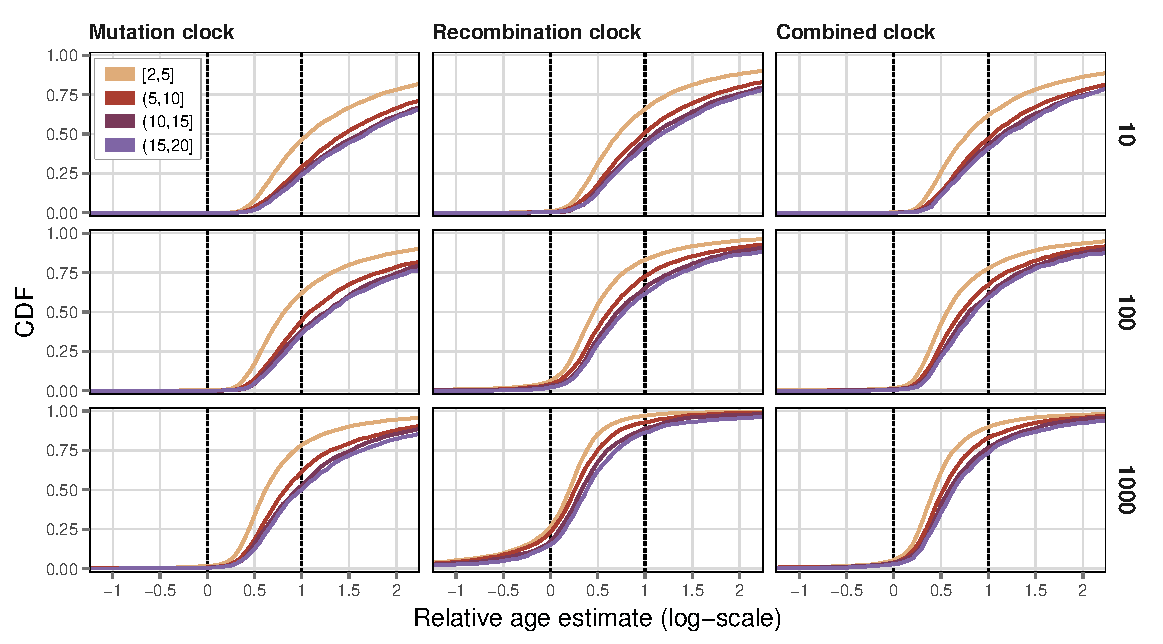
\includegraphics[width=\textwidth]{./img/ch5/discords_hist}
\Caption{Relative age under varying numbers of discordant pairs}
{A randomly drawn set of \n{10000} target sites at allele frequency ${\leq 1\%}$, \ie \fk{[2,20]}, was analysed under each of the \n{3} clock models (indicated at the \emph{top} of each column) and with different numbers of sampled discordant pairs; ${n_d = \num{10}}$, ${n_d = \num{100}}$, and ${n_d = \num{1000}}$ (indicated at the \emph{right} of each row).
The analysis was conducted using the true IBD breakpoints as derived from simulation records, defined as the first variant sites observed in the data that immediately follow the \n{2} recombination events on each side distal to a given focal site.
The relative age, ${\hat{t}_\textit{rel}}$, was calculated as given in \cref{eq:age_relative}, such that the true times of concordant and discordant coalescent events, $t_c$ and $t_d$, sit at 0~and~1, respectively (\emph{dashed} lines).
Note that ${\hat{t}_\textit{rel}}$ is defined on log-scale.
The \gls{cdf} of relative age estimates is shown per \fk{}~group, where target variants were pooled by their allele count in the data, in ranges of \fk{[2,5]}, \fk{(5,10]}, \fk{(10,15]}, and \fk{(15,20]}.}
{fig:discords_hist}
\end{figure}

%

A comparison of the inferred age distributions at distinct \fk{}~ranges is presented in \cpref{fig:discords_hist}, again shown for ${n_d = \num{10}}$, ${n_d = \num{100}}$, and ${n_d = \num{1000}}$.
Notably, the accuracy of target alleles at lower frequencies was overall higher compared to alleles observed at higher frequencies.
This difference was consistent across $n_d$ thresholds under the mutation clock model, \ClockM.
For example, at ${n_d = \num{10}}$, the proportion of correctly dated alleles was higher in the \fk{[2,5]} range (\SI{48.35577}{\percent}) compared to alleles at \fk{(5,10]} (\SI{29.44512}{\percent}).
At ${n_d = \num{1000}}$, overall accuracy was increased but the difference for alleles at lower and higher frequencies remained; \ie \SIlist{77.81947;60.83435}{\percent} at \fk{[2,5]} and \fk{(5,10]}, respectively.
Under the recombination clock model, \ClockR, these differences were reduced at higher $n_d$ thresholds.
At ${n_d = \num{10}}$, \SIlist{66.60781;50.34427}{\percent} of alleles were correctly dated at \fk{[2,5]} and \fk{(5,10]}, respectively, whereas at ${n_d = \num{1000}}$ these proportions were \SIlist{72.25778;69.82584}{\percent} at the same frequency ranges, respectively.

% To explain this observation, consider the genealogical relationship of the sample that is distinguished into $X_c$ and $X_d$ dependent on sharing and non-sharing of a given focal allele, respectively.
% If the focal allele frequency is low, the number of coalescent events that precede the focal mutation event is larger compared to a focal allele shared at a higher frequency in the sample.
% Therefore, a higher $n_d$ threshold increases the chance to randomly


%
\subsection{Discussion}
%


In summary, the method as well as the clock models proposed were able to estimate allele age from IBD information alone, without prior knowledge of the demographic history of the sample.
However, because data were simulated under a simple demographic model (dataset $\mathcal{D}_A$), further evaluation is appropriate (\eg using datasets $\mathcal{D}_B$ and $\mathcal{D}_B^{\ast}$; see next section).
The analysis considered true IBD segments and therefore evaded the effects that would result from inexact IBD detection.
Since true IBD was determined conditional on the observed variation in the data, the analysis reflected the practical feasibility of age estimation given available data.


The implemented sampling regime for discordant pairs sought to find a compromise between computational tractability and the chance of randomly selecting haplotypes that are informative for the estimation.
However, ideally, to minimise the computational burden while simultaneously improving estimation accuracy, it would be desirable to consider the nearest neighbours to the focal shared haplotypes in the local genealogy.
If the nearest neighbours are found among the haplotypes in $X_d$ and paired with the focal haplotypes in $X_c$ they are likely to coalesce \Correct{more closely} to $t_d$ and would therefore be more informative for the estimation of focal allele age.

For instance, a simple approach would be to compute the Hamming distance between haplotypes in $X_c$ and $X_d$ within a short region around the position of a given target site, such that a subset of presumed nearest neighbours can be selected based on a distance ranking.
In practice, however, there are \Correct{two} caveats to such an approach.
First, it would be computationally expensive to conduct an additional pairwise analysis for the (whole) sample at each target site, which may not outweigh the improvement gained through the reduction of $n_d$.
\Correct{Second,} a dilemma arises in presence of data error, as the identification of nearest neighbours is likely to give preference to haplotypes in which the focal allele has been missed.
\label{p:falseneg}%
Such \emph{false negatives} distort the estimation of allele age as the \gls{ccf}
computed for false discordant pairs could bias the resulting composite posterior distribution.
% In such cases, the estimated age is expected to be approximately equal to or smaller than $t_c$, such that $\hat{t}$ is likely to be underestimated.

It is important to note that the problem of finding false negatives in the data cannot be avoided if discordant pairs are formed by a random sampling process, but the chance of including false negatives is reduced if $n_d$ is small in comparison to the (haploid) sample size.
Hence, the $n_d$ threshold defines a balance between accuracy and expected bias.

% In the following, analyses were conducted using a threshold equal to the diploid sample size, $N$; that is ${n_d = \num{1000}}$ in analyses using $\mathcal{D}_A$, and ${n_d = \num{2500}}$ using $\mathcal{D}_B$ or $\mathcal{D}_B^{\ast}$.
% Since the results presented in this section were obtained on true IBD information, they serve as a benchmark against which different IBD detection methods are compared in the section below.













%
\section{Age estimation using inferred shared haplotype segments}
%


The \texttt{tidy} algorithm for targeted IBD detection (see Chapters~3 and 4) was fully integrated in \texttt{rvage}, such that several methods for IBD detection were available to inform allele age estimation;
namely the \gls{fgt}, \gls{dgt}, and the \Correct{genotype-based} \gls{hmm}.

In this section, \n{2} main analyses were conducted.
First (\cref{sec:compare_ibd_methods}), dataset $\mathcal{D}_A$ was analysed to provide a comparison to \cpref{sec:age_validation_analysis}, where true shared haplotype information was used to validate the age estimation method.
Second (\cref{sec:age_generror}), an extensive analysis was performed on datasets $\mathcal{D}_B$ and $\mathcal{D}_B^{\ast}$ to assess the impact of data error on age estimation.
\Addition{Note that the impact of phasing error was also evaluated in the latter, but which affected only the \gls{fgt}.}

The IBD detection methods used here were originally designed to infer shared haplotype segments in individuals sharing a focal allele.
While this condition is fulfilled when considering concordant pairs, the IBD detection in discordant pairs is problematic.
\Correct{In the section below, I describe the modifications made to infer shared haplotypes in discordant pairs.}


%
\subsection{Modifications of IBD detection methods}
%

\paragraph{\Glsentryfull{fgt}.}
The \gls{fgt} is applied to the \n{4} haplotypes observed in \n{2} diploid individuals.
A recombination event is inferred to have occurred between \n{2} variant sites if all \n{4} possible allelic configurations are observed.
Let the focal site be denoted by $b_i$ and another, distal site by $b_j$.
In the \n{4} haplotypes, the alleles observed at ${(b_i,b_j)}$ confirm a breakpoint if, for example, ${(0,0)}$, ${(1,0)}$, ${(0,1)}$, and ${(1,1)}$ are observed, where $0$ denotes the ancestral allelic state and $1$ the derived state.
Since breakpoints are inferred on both sides of a given focal variant, the genotypes at the focal site are both heterozygous in concordant pairs.
But because the \n{2} individuals considered in a discordant pair do not share the focal allele, the required configuration cannot be observed.

%
%!TEX root = ../../main.tex


\begin{figure}[!htb]
\centering
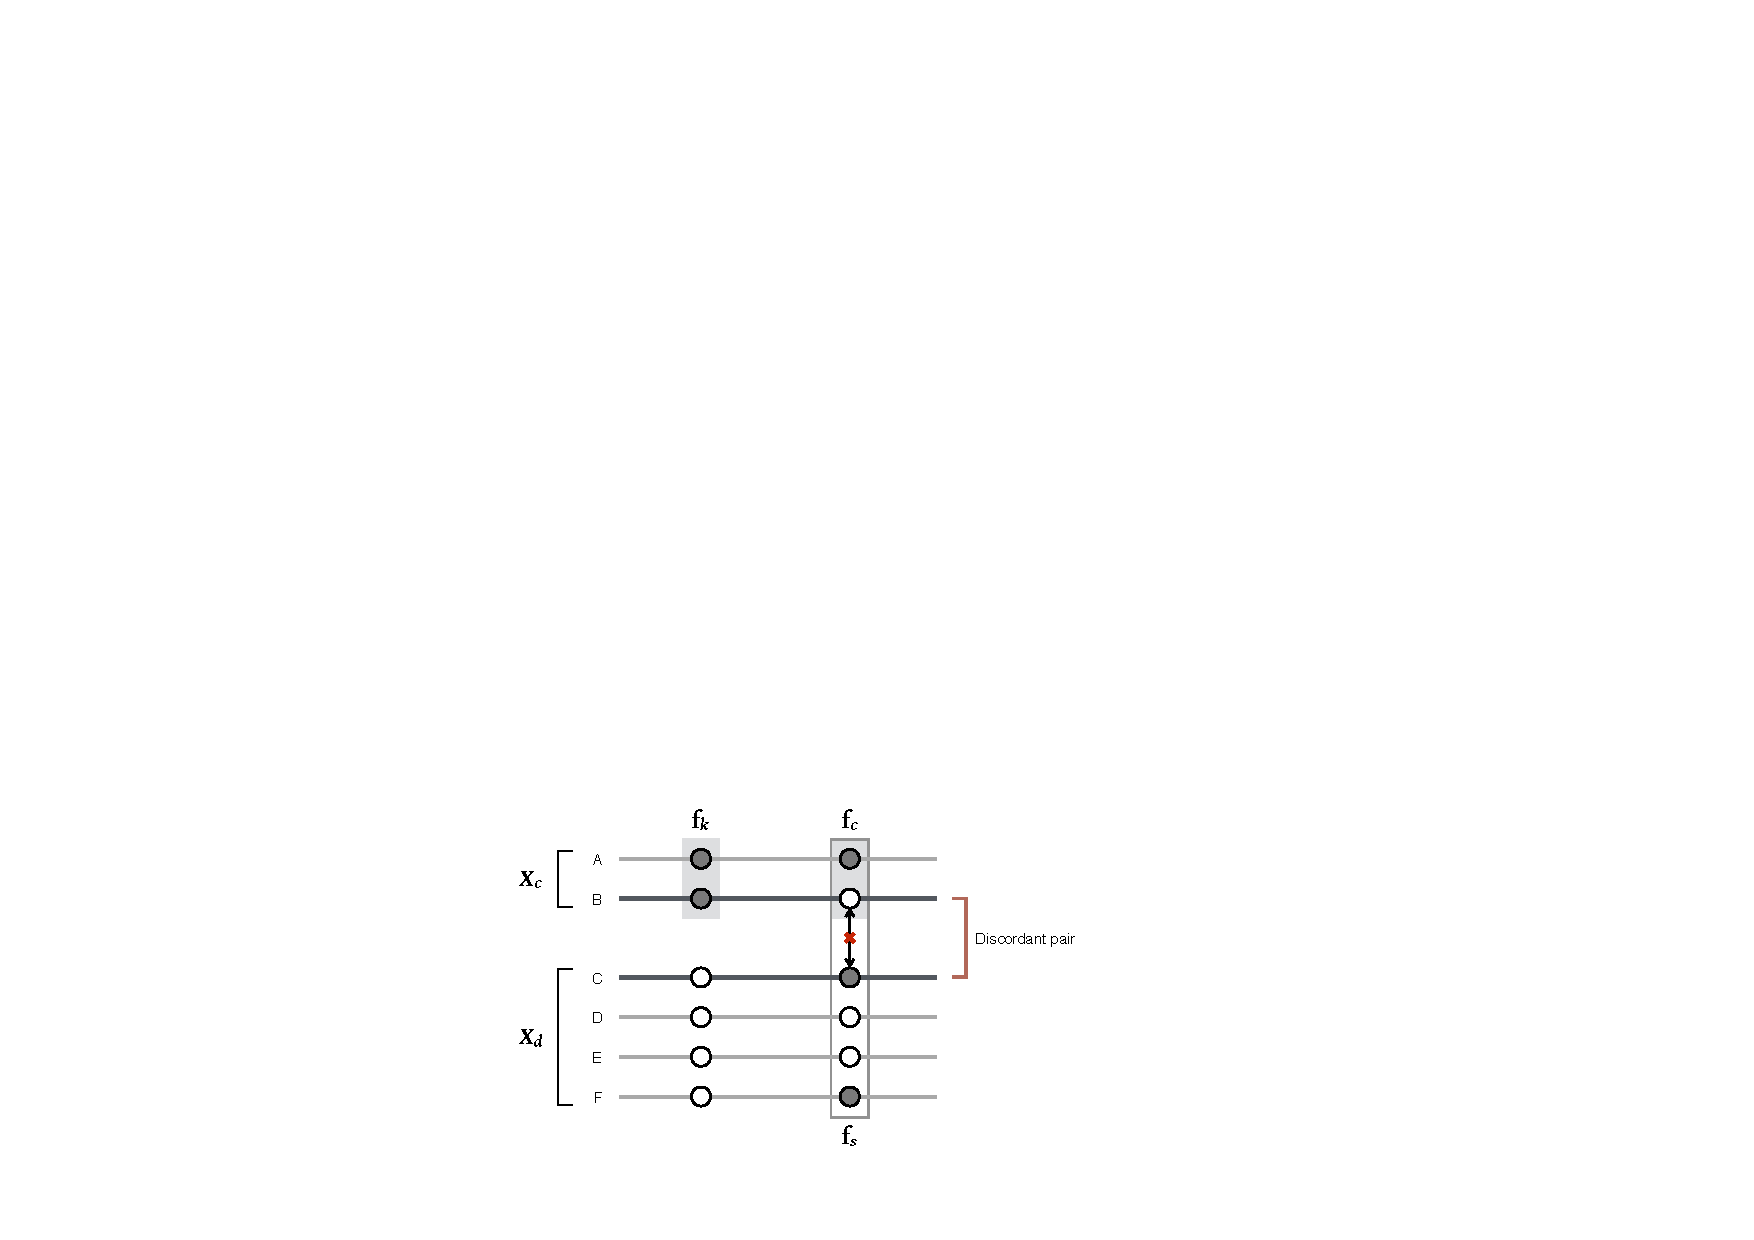
\includegraphics[width=0.7\textwidth]{./img/ch5/info_fgt_discord}
\Caption{Breakpoint detection in discordant pairs}%
{A discordant pair is formed by \n{1} haplotype from $X_c$ (which share the focal allele) and \n{1} haplotype from $X_d$ (which do not share the focal allele).
The lines indicate the chromosomal sequence where the alleles at \n{2} sites are indicated; allelic states are distinguished as the ancestral (\emph{hollow} circle) and derived state (\emph{solid}).
The conditions that lead to the detection of a recombination breakpoint is indicated between the focal site (\emph{left}) and another, distal site (\emph{right}), where \fk{} denotes the number of allele copies at the focal site within the subsample $X_c$, \fk{c} denotes the number of allele copies observed at the distal site within the subsample $X_c$, and \fk{s} denotes the number of allele copies at the distal site within the whole sample.
The \gls{fgt} is passed if all \n{4} allelic configurations are observed at \n{4} haplotypes in the sample.}%
{fig:info_fgt_discord}
\end{figure}

%

\Correct{However, breakpoints in discordant pairs can be detected as based on the allele frequencies observed in the sample.}
Let \fk{} denote the number of allele copies at focal site $b_i$.
At a distal site, $b_j$, let \fk{c} denote the number of allele copies observed only within the subsample $X_c$ \Correct{(who carry the focal allele at the focal position)}.
Also, let \fk{s} be the number of allele copies \Correct{at $b_j$} in the whole sample.
A recombination breakpoint is indicated at $b_j$ if the \n{2} haplotypes carry different alleles and if ${\fk{c} < \fk{}}$ and ${\fk{c} < \fk{s}}$; additionally ${\fk{s} > 1}$ to exclude singletons and ${(\fk{s} - \fk{c}) > (2N - \fk{})}$ to exclude sites that are monomorphic within $X_d$, where $2N$ refers to the number of haplotypes in the sample.
The condition implies the existence of the \n{4} allelic configurations at any of the haplotypes in the sample but is not bound by haplotype occurrence in \n{2} diploid individuals.
The \gls{fgt} thereby still holds but is practically inverted.
An example is illustrated in \cpref{fig:info_fgt_discord}.


\paragraph{\Glsentryfull{dgt}.}
Recall that the \gls{dgt} is a special case of the \gls{fgt} which detects breakpoints at genotypic configurations that would also pass the \gls{fgt} if haplotypes were available.
Given the \n{2} heterozygous genotypes at the focal variant, a breakpoint is found at a distal site if opposite homozygous genotypes are observed.
%; for example, ${(1,0)}$ and ${(1,2)}$, where $0$ denotes a genotype homozygous for the ancestral allele, $1$ a heterozygous genotype, and $2$ a genotype homozygous for the derived allele.
Again, in discordant pairs, such a configuration cannot be observed.
The observation of opposite homozygous genotypes nonetheless implies that the \n{2} individuals do not share a haplotype at this site and is therefore also applied for breakpoint detection in discordant pairs.

%
%!TEX root = ../../main.tex


\begin{figure}[!htb]
\centering
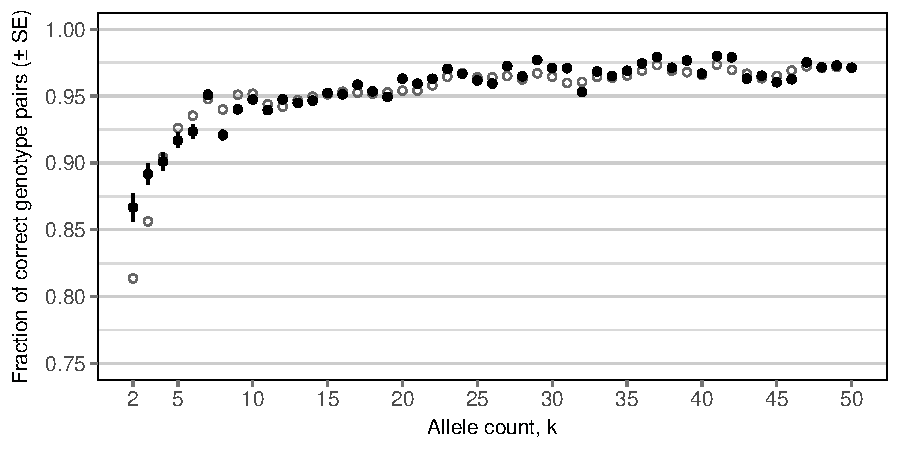
\includegraphics[width=0.8\textwidth]{./img/ch5/info_hmm_discord}
\Caption{Initial state probability of discordant pairs in the Hidden Markov Model (HMM)}%
{The proportion of discordant pairs that were correctly identified by their genotypes was empirically determined from data before and after the inclusion of realistic genotype error rates.
The mean per \fk{} was used as the initial state probability of the \gls{hmm}-based approach for IBD detection around target sites.
For comparison, the initial state probability of concordant pairs is shown (\emph{hollow} circles).}%
{fig:info_hmm_discord}
\end{figure}

%

\paragraph{Genotype-based \glsentrylong{hmm}.}
The \gls{hmm} includes a probabilistic model for observing each possible genotype pair in pairs of diploid individuals in \emph{ibd} and \emph{non}, which are the hidden states defined in the underlying IBD model; see Chapter~4.
Both the emission and initial probabilities were determined empirically, from data before and after the inclusion of realistic genotype error rates.

The initial state probability corresponds to the probability of correctly observing a concordant pair through allele sharing, \ie the true positive rate of observing heterozygous genotypes at a given target site where both individuals share the focal allele, which was determined per focal allele frequency (\fk{}).
The \Correct{empirical model was extended such that there was an additional initial state probability available and applied to} discordant pairs.
\Correct{By comparing the data before and after error ($\mathcal{D}_B$~and~${\mathcal{D}_B}^{\ast}$), the initial state probability was determined as follows.}
For each \fk{}~category, I randomly selected \n{1000} target sites in the dataset ``before error'' for which I randomly selected \n{1000} discordant pairs per target site.
I then compared these genotypes to the corresponding genotypes in the dataset ``after error'' to determine the true positive rate.
The mean per \fk{} was taken as the empirical initial state probability.
The resulting distribution is shown in \cpref{fig:info_hmm_discord}; the initial state probabilities used for discordant pairs are given for comparison.
However, the initial state probability for the discordant case is similar to the concordant one.
A possible explanation is that this is particularly driven by the heterozygous status being false.

\Addition{The same empirical emission model was applied to discordant pairs as it follows from the coalescent (under the assumption of the infinite sites model) that the relationship at any site in the genome can be traced back to a common ancestor if looking back far enough.
However, it must be noted that the current model was constructed to consider recent IBD.
It can be expected that inference at discordant pairs is therefore less accurate.}


Note that both the \gls{dgt} and the \gls{hmm}-based approach may operate on genotype data alone.
Importantly, if haplotype information is not available, the sets $X_c$ and $X_d$ are formed by assigning all individuals that are heterozygous to $X_c$ while all others are assigned to $X_d$, but excluding individuals that are homozygous for the focal allele.
% This may reduce the information available from the sample, but the effect is expected to be negligible if the focal allele is rare.
Since haplotype data are required to determine pairwise differences along haplotype sequences, \ClockM and \ClockC cannot be used with genotype data.
\Correct{Here, analyses using the \gls{dgt} and the \gls{hmm}-based approach were performed on haplotypes although genotype data alone would suffice.}





%
\subsection{Comparison of IBD detection methods}\label{sec:compare_ibd_methods}
%

Dataset $\mathcal{D}_A$ was used to compare the different IBD detection methods.
Age was estimated for each of the \n{3} clock models, using a threshold of ${n_d=\num{1000}}$.
The results presented in this section were obtained on the previously selected \n{10000} rare allele target sites; see \cpref{sec:age_validation_analysis}.
Again, the parameters of the age estimation method were specified according to simulation parameters (${\Ne=\num{10000}}$; ${\mu=\num[round-precision=1]{1e-08}}$ per site per generation; ${\rho=\num[round-precision=1]{1e-08}}$ per site per generation).



% Note that genotype data are sufficient for IBD detection using the \gls{dgt} and \gls{hmm}, but haplotypes are required for estimation under the mutation clock model; \ie to count pairwise differences, $S$, along haplotype sequences.
% Thus, analyses were conducted on the simulated haplotype dataset ($\mathcal{D}_A$), but haplotype phase was ignored during IBD detection in the \gls{dgt} and \gls{hmm}.
% Here, because simulated data did not include genotype error, theoretical emission model was used in the \gls{hmm}.



% , which were analysed using each of the \n{3} IBD detection methods and under each clock model, resulting in a total of \dec{93.295215}~million pairwise analyses.

% The fraction of conflicting age estimates differed by clock model as well as IBD detection method; no conflicting estimates were returned when true IBD was used.
% Under the mutation clock, \ClockM, analyses using the \gls{fgt} returned \SI{1.808575}{\percent} conflicts.
% This fraction was higher using the \gls{dgt} and \gls{hmm}, with \SIlist{2.601097;2.326762}{\percent}, respectively.
% Conflicts were seen less under the recombination clock, \ClockR, where none were returned using the \gls{fgt}, but \SIlist{0.010160;0.030481}{\percent} using the \gls{dgt} and \gls{hmm}.
% The fraction under the combined clock, \ClockC, was smaller compared to \ClockM, with
% \SIlist{1.097337;2.265799;1.818736}{\percent} of conflicted sites using the \gls{fgt}, \gls{dgt}, and \gls{hmm}, respectively.
% The remaining sites were intersected to compare clock models and IBD methods on the same set of target sites, retaining \n{9434} variants.

%
% !TEX root = ../../main.tex


\begin{figure}[!htb]
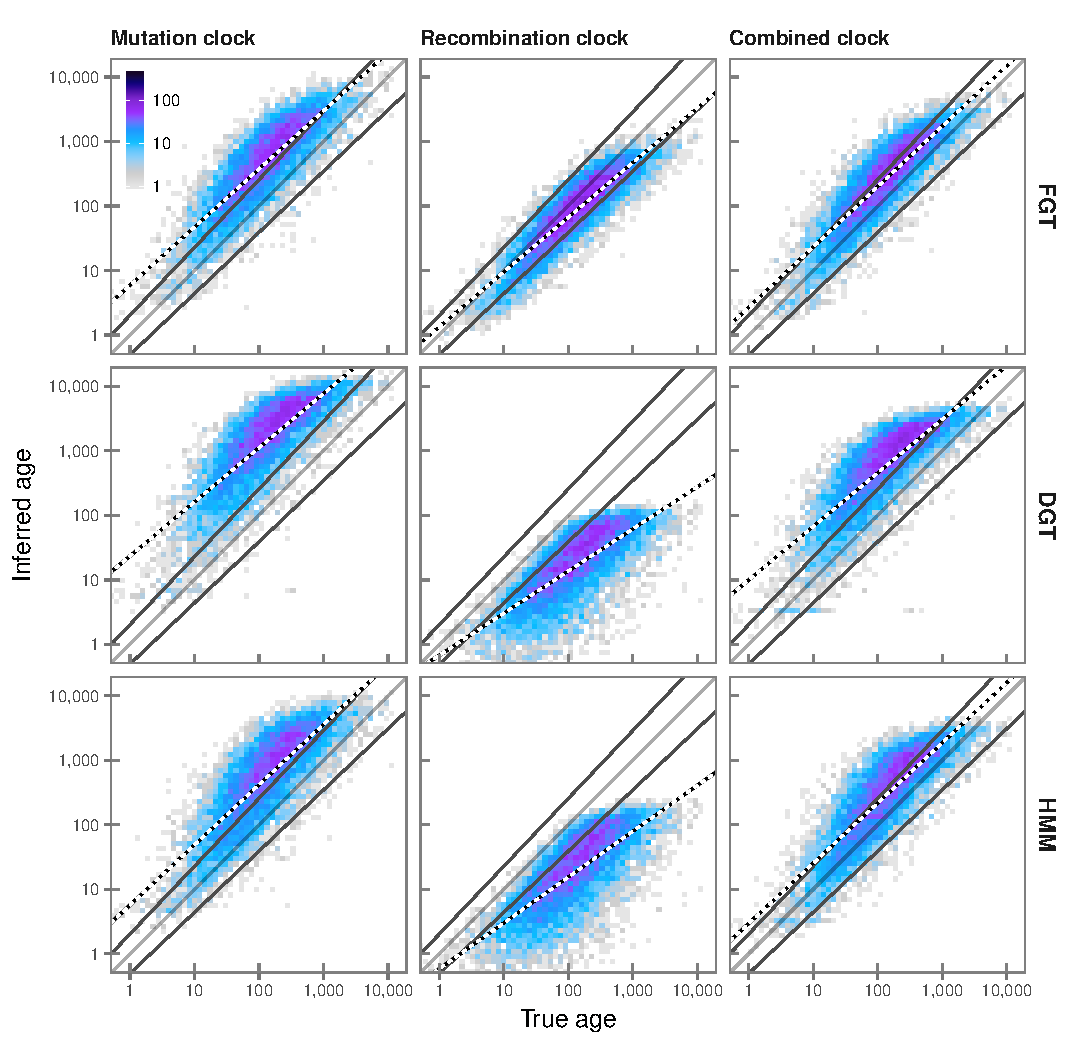
\includegraphics[width=\textwidth]{./img/ch5/vanilla_scat}
\Caption{Distribution of true and inferred age using different IBD detection methods}
{The \n{3} IBD detection methods \gls{fgt}, \gls{dgt}, and \gls{hmm} were compared under each clock model, on the same set of target sites that were drawn from \fk{[2,20]} variants (allele frequency ${\leq 1\%}$) in $\mathcal{D}_A$.
Each panel shows the density of true age ($t_m$) and inferred age.
Lines \emph{below} and \emph{above} the dividing line are regression trend lines of the corresponding true coalescent times around each mutation event, $t_c$ and $t_d$, respectively.
The regression of inferred age ($\hat{t}$) is given by the \emph{black-white} line.}
{fig:vanilla_scat}
\end{figure}

%

The density of true and inferred allele age is given in \cpref{fig:vanilla_scat}.
In all \n{3} methods, a tendency to overestimate allele age was seen, in particular under the mutation clock, \ClockM.
This overestimation was elevated when the \gls{dgt} was used, and less prominent for the \gls{fgt} or \gls{hmm}.
The latter methods showed similar distributions in \ClockM and under the combined clock model, \ClockC, in which age appeared to be less overestimated.
Under the recombination clock, \ClockR, alleles were underestimated in each method, but more severely in both the \gls{dgt} and \gls{hmm}.

Specifically, the method with the highest proportion of correctly estimated alleles was the \gls{fgt} in all \n{3} clock models, where accuracy was highest under \ClockR (\Percent{72.609710}), followed by \ClockC (\Percent{55.39538}) and \ClockM (\Percent{34.46046}).
The \gls{hmm} achieved similar proportions, but which was low in \ClockR (\SI{10.949756}{\percent}) compared to \ClockC (\SI{51.87619}{\percent}) and \ClockM (\SI{32.41467}{\percent}).
Throughout, the lowest proportions were found for the \gls{dgt} (\SIlist{14.55374;8.225567;29.65868}{\percent} for \ClockM, \ClockR, and \ClockC, respectively).
% , which also showed the lowest proportion in \ClockR (\SI{8.225567}{\percent}) and comparatively low levels of accuracy in \ClockM and \ClockC (\SIlist{14.55374;8.225567;29.65868}{\percent}, respectively).
% Overestimation of allele age was highest in \ClockM, where \SIlist{65.08374;85.27666;66.95993}{\percent} of alleles were underestimated by the \gls{fgt}, \gls{dgt}, and \gls{hmm}, respectively.
% Conversely, the proportion of underestimated alleles was lowest in \ClockM, at ${\leq 1\%}$ in each method, and similarly low in \ClockC with ${\leq 2\%}$ in each method.
% In contrast, alleles were markedly underestimated in \ClockR; the \gls{fgt} resulted in \SI{20.13992}{\percent} of underestimated alleles, whereas \SIlist{91.75323;88.93364}{\percent} of alleles were underestimated when the \gls{dgt} and the \gls{hmm} were used for IBD inference, respectively.

%
% !TEX root = ../../main.tex


\begin{table}[!htb]
\Caption{Estimation accuracy per IBD detection method}
{The accuracy was measured in analyses based on IBD detected by different methods; namely the \gls{fgt}, \gls{dgt}, and the \gls{hmm}-based approach.
See \cpref{tab:stats_discords} for comparison to results obtained using true IBD segments (for ${n_d = \num{1000}}$).}
{tab:stats_vanilla}
\centering
\begin{tabular}{cl*6{S[table-format=1.3]}}
\toprule
Clock & Method &
\multicolumn{3}{c}{Rank correlation ($r_S$)} &
\multicolumn{3}{c}{RMSLE} \\
\cmidrule(lr){3-5}
\cmidrule(lr){6-8}
& & {$t_c$} & {$t_m$} & {$t_d$} & {$t_c$} & {$t_m$} & {$t_d$} \\
\otoprule
\ClockM &  FGT  & \bfseries 0.840676 & \bfseries 0.839366 & \bfseries 0.686220  &  \bfseries 1.011494 & \bfseries 0.652508 & \bfseries 0.554208  \\
        &  DGT  &  0.829831 & 0.812906 & 0.650413  &  1.460099 & 1.085978 & 0.832110  \\
        &  HMM  &  0.805637 & 0.806060 & 0.661580  &  1.077573 & 0.725273 & 0.606789  \\
\cmidrule(lr){1-8}
\ClockR &  FGT  &  \bfseries 0.898918 & \bfseries 0.886870 & \bfseries 0.717613  &  \bfseries 0.338500 & \bfseries 0.329674 & \bfseries 0.774566  \\
        &  DGT  &  0.819520 & 0.749442 & 0.553535  &  0.576894 & 0.940863 & 1.396338  \\
        &  HMM  &  0.820884 & 0.751320 & 0.555899  &  0.532765 & 0.891761 & 1.348435  \\
\cmidrule(lr){1-8}
\ClockC &  FGT  &  \bfseries 0.863498 & \bfseries 0.873015 & \bfseries 0.723484  &  \bfseries 0.754705 & \bfseries 0.422342 & \bfseries 0.523968  \\
        &  DGT  &  0.839769 & 0.828786 & 0.669072  &  1.083494 & 0.726881 & 0.600412  \\
        &  HMM  &  0.825717 & 0.834311 & 0.692021  &  0.806485 & 0.485257 & 0.553758  \\
\bottomrule
\end{tabular}
\end{table}

%

Summary metrics for each analysis are given in \cpref{tab:stats_vanilla}.
Throughout, the \gls{fgt} showed a higher accuracy compared to the other IBD detection methods under each clock model.
% under the recombination clock model, \ClockR, showed a higher correlation and slightly reduced error with regard to $t_d$.
% There, rank correlation was ${r_S = \dec{0.898918}}$ for the \gls{fgt} and ${r_S = \dec{0.888794}}$ for true IBD; likewise the magnitude of error (\gls{rmsle}) was \dec{0.338500} and \dec{0.345374} for \gls{fgt} and true IBD, respectively.
% However, note that a higher accuracy at $t_c$ does not necessarily reflect an improvement in the estimation of actual allele age.
% For example, the accuracy with regard to $t_m$ or $t_d$ was lower for the \gls{fgt} compared to true IBD.
% In comparison to the other detection methods, the \gls{fgt} outperformed both the \gls{dgt} and \gls{hmm} with regard to each time measure.
% The \gls{hmm} showed slightly higher levels of accuracy than the \gls{dgt} in \ClockR, where $r_S$ was higher and \gls{rmsle} lower in terms of each time measure for the \gls{hmm}.
% Similarly, in both \ClockM and \ClockC, \gls{rmsle} scores were lower for the \gls{hmm} compared to the \gls{dgt}, whereas $r_S$ measures were similar.
Relative age estimates are shown for distinct \fk{}~ranges in \cpref{fig:vanilla_hist}, where the relative age for corresponding results obtained by using true IBD information is given for comparison per clock model; see \cpref{fig:discords_hist}.
Analyses under \ClockM and \ClockC showed a substantial difference between alleles at lower and higher frequencies; \eg overall accuracy of \fk{[2,5]} variants was increased compared to \fk{}~variants at higher frequencies in each method.
This difference was reduced under \ClockR, but the \gls{dgt} showed an accuracy decrease for \fk{[2,5]} variants.

%
% !TEX root = ../../main.tex


\begin{figure}[!htb]
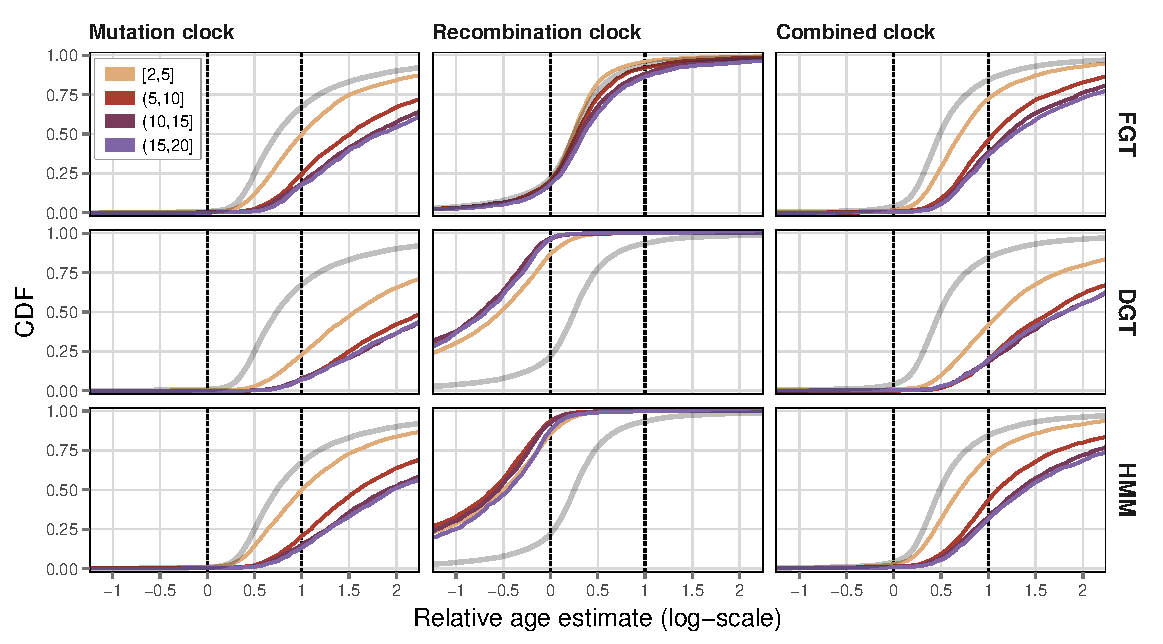
\includegraphics[width=\textwidth]{./img/ch5/vanilla_hist}
\Caption{Relative age using different IBD detection methods}
{The \n{3} IBD detection methods implemented in \texttt{rvage} were compared, \ie \gls{fgt}, \gls{dgt}, and \gls{hmm} (indicated at the \emph{right} of each row), under each clock model (indicated at the \emph{top} of each column).
The relative age, ${\hat{t}_\textit{rel}}$, was calculated as given in \cref{eq:age_relative}, such that $t_c$ and $t_d$ sit at 0~and~1 (\emph{dashed} lines).
The \gls{cdf} of relative age estimates is shown for different frequency ranges; namely \fk{[2,5]}, \fk{(5,10]}, \fk{(10,15]}, and \fk{(15,20]}.
\Correct{The \emph{grey} line provides a comparison to age estimated using true IBD information as shown in \cpref{fig:discords_hist}, but for \fk{[2,20]}.}}
{fig:vanilla_hist}
\end{figure}

%


% %
% % !TEX root = ../../main.tex


\begin{figure}[!htb]
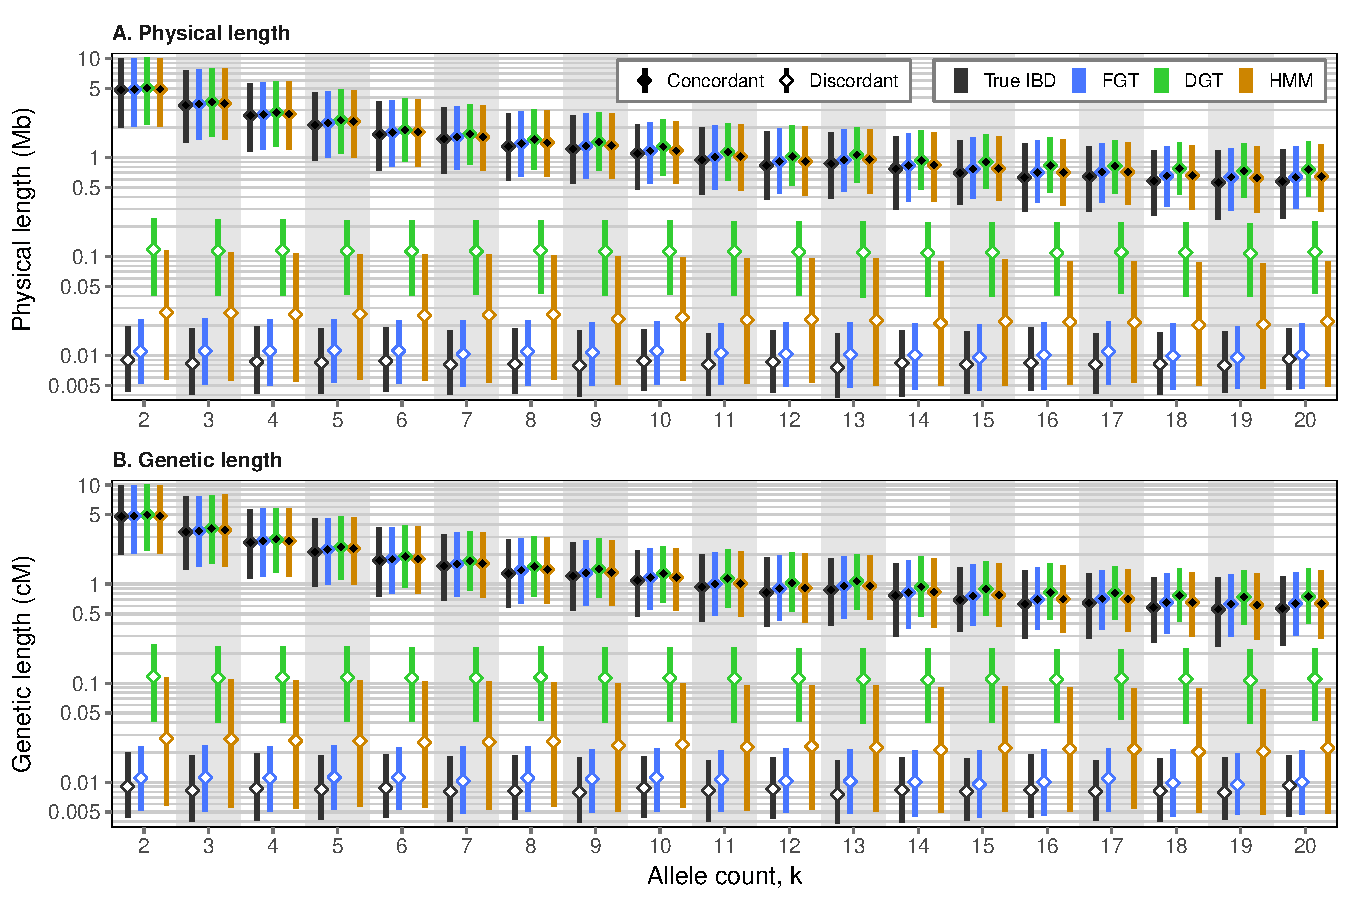
\includegraphics[width=\textwidth]{./img/ch5/vanilla_length_con_dis}
\Caption{Length distribution of inferred IBD segments}
{Bottom and top of each bar indicate \nth{1} and \nth{3} quartiles, respectively, between which the median (\nth{2} quartile) is marked (\emph{diamonds}).
IBD detected for concordant and discordant pairs is distinguished; \emph{solid} and \emph{hollow} diamonds, respectively.}
{fig:vanilla_length_con_dis}
\end{figure}

% %
%
% The distribution of IBD lengths inferred using the \gls{fgt}, \gls{dgt}, and the HMM-based approach are shown in \cpref{fig:vanilla_length_con_dis}.
% Segments inferred using the HMM were close to those detected using the \gls{fgt} in concordant pairs.
% However, for discordant pairs, only the \gls{fgt} produced IBD segments that were close to the length distribution of true IBD segments.
% The \gls{dgt} showed the highest degree of overestimation for both concordant and discordant pairs.



These results suggested that the accuracy of estimated allele age is crucially dependent on correct inference of the underlying IBD structure.
\Correct{The clock models behave differently when the length of an IBD segment is over or underestimated.}
It can be expected that \ClockM may indicate an older allele age if IBD length is overestimated, due to potentially including a larger number of mutational differences which suggests an older \gls{tmrca}.
Conversely, \ClockR may indicate a younger age, because a more recent \gls{tmrca} is suggested when IBD length is relatively long.

% The overestimation of IBD lengths, which is generally expected for each method, affected each clock model differently.
% While \ClockM overall resulted in an overestimation of allele age when IBD is overestimated, this pattern was reversed in \ClockR.
% Although both models are combined in \ClockC, the impact of mutational differences, seen at the overestimated regions of detected IBD segments, was substantial and could not be mitigated by considering recombinational length.

I found that the \gls{fgt} was the best performing method for the targeted detection of IBD segments, as the accuracy of estimated age was similar to the expectations defined by true IBD information in \cref{sec:age_validation_analysis}.
However, the estimation was more accurate for target sites at lower allele frequencies.
The \gls{dgt} was least accurate in terms of estimated allele age in this comparison.

Recall that the probabilistic model of the \gls{hmm} was developed to overcome the effects of genotype error encountered in real data (see Chapter~4).
Thus, the results in this section reflect theoretical limitations of age estimation given IBD detected in flawless data, but may change drastically in presence of genotype error.
This was explored in the section below.



%
\subsection{Impact of genotype error on allele age estimation}
\label{sec:age_generror}
%

Allele age was estimated using datasets $\mathcal{D}_B$~and~$\mathcal{D}_B^{\ast}$, to compare the accuracy of the estimation method before and after error.
\Addition{Shared haplotype inference was performed using the \gls{fgt}, \gls{dgt}, and the genotype-based \gls{hmm}.
In addition, age was estimated using true IBD information as determined from simulation records.}

In total, \n{5000} target sites were randomly selected at allele frequency ${\leq 0.5\%}$ (\fk{[2,25]}).
Note that these were sampled from the subset of variants unaffected by error in $\mathcal{D}_B^{\ast}$, to ensure that alleles correctly identified haplotype sharing.
A threshold of ${n_d = \num{2500}}$ was applied to randomly select concordant pairs at a given target site.
\Correct{Note that statistically phased data was available for both $\mathcal{D}_B$ and $\mathcal{D}_B^{\ast}$, which were included here to assess the impact of phasing error, but which can only affect the \gls{fgt}.}

% The allele age estimation method was evaluated under each clock model and each method for IBD detection, on data before and after the inclusion of genotype error; \ie using datasets ${\mathcal{D}_B}$ and ${\mathcal{D}_B^{\ast}}$, respectively.
% A set of \n{10000} target sites selected at \fk{[2,25]} in a sample of ${N = \num{2500}}$ diploid individuals, using a threshold of ${n_d = \num{2500}}$, which amounted to \dec{25.281233}~million pairwise analyses per comparison.
% The \gls{fgt} was applied to both the simulated (\emph{true}) haplotypes as well as phased haplotype data.
% The \gls{hmm} used theoretical emission model in analyses on ${\mathcal{D}_B}$ and the empirical error model in analyses on ${\mathcal{D}_B^{\ast}}$.
% To measure accuracy, true IBD segments were determined from simulation records and separately analysed on the same number of concordant and discordant pairs in data before and after error.
% In total, for the results presented in this section, \dec{758.43699}~million pairwise analyses were conducted.

% %
% % !TEX root = ../../main.tex


\begin{table}[!htb]
\Caption{Conflicted estimates in analyses before and after error}
{}
{tab:stats_conflicts}
\centering
\begin{threeparttable}
\begin{tabular}{l*6{S[table-format=2.3]}}
\toprule
 Method &
 \multicolumn{3}{c}{Conflicts before error (\%)} &
 \multicolumn{3}{c}{Conflicts after error (\%)} \\
\cmidrule(lr){2-4}
\cmidrule(lr){5-7}
  &  {\ClockM} & {\ClockR} & {\ClockC}  &  {\ClockM} & {\ClockR} & {\ClockC} \\
\otoprule
FGT*       &   6.396224 & 0.000000 & 3.695150  &   5.131037 & 0.140576 & 2.188974 \\
FGT**      &   6.587006 & 0.421729 & 4.387990  &   4.940255 & 0.341399 & 3.122803 \\
DGT        &  10.944874 & 0.160658 & 8.384375  &   5.211366 & 1.767245 & 3.956220 \\
HMM        &   5.884124 & 0.391605 & 4.418114  &  13.334672 & 0.823375 & 9.267998 \\
\cmidrule(lr){1-7}
True IBD   &   0.000000 & 0.000000 & 0.000000  &   9.583101 & 0.000000 & 1.030332 \\
\bottomrule
\end{tabular}
\begin{tablenotes}\footnotesize
	\item[{${\ast}$}] ~ FGT applied to true haplotypes
	\item[{${\ast\ast}$}] ~ FGT applied to phased haplotypes
\end{tablenotes}
\end{threeparttable}
\end{table}

% %
% As in the previous section, some of the analyses returned conflicting estimates; see \cref{tab:stats_conflicts}.
% Again, no conflicts were seen when true IBD information was used.
% However, this changed after the inclusion of genotype error; the fraction of conflicting estimates was high in \ClockM, zero in \ClockR, and small in \ClockC.
% Before error, the largest fraction of conflicts was seen for the \gls{dgt} in \ClockM.
% Data from analyses before and after error were intersected across results obtained under each clock model and for each IBD method, which retained a set of \n{5015} identical target sites.
% A complete summary of the accuracy per analysis is given below in \cpref{tab:stats_generror}.

%
\subsubsection{Age estimation using true shared haplotype information}
%

%
% !TEX root = ../../main.tex


\begin{figure}[tb]
{\small\texthv{\textbf{\,(a) True IBD}}} \\
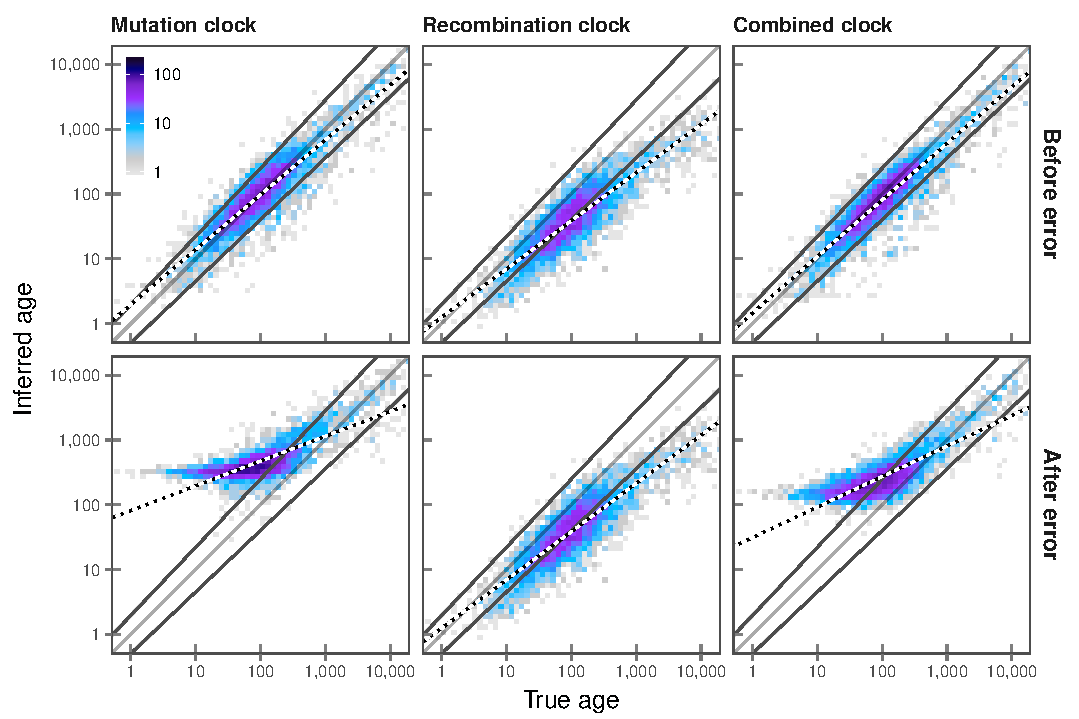
\includegraphics[width=\textwidth]{./img/ch5/generror_scat_tru}
\Caption{Density of allele age before and after error in simulated data}
{The effects on the estimation process \emph{before} and \emph{after} error are compared.
Note that the ``true age'' was set to $t_m$, which is the geometric mean of $t_c$ and $t_d$.
Lines \emph{below} and \emph{above} the dividing line correspond to the regression lines over $t_c$ and $t_d$; \ie of the times of coalescent events delimiting the branch on which a focual mutation occurred.
The \emph{black-white} line gives the regression for the inferred age ($\hat{t}$).
This panel (\textbf{a}) compares the distributions of true and inferred ages, which were estimated on basis of the true IBD structure of the sample as determined from simulation records.
The other panels show estimation results based on the different IBD detection methods;
\gls{fgt} on both true and phased haplotypes (\textbf{b}, \textbf{c}; \pref{fig:generror_scat_fgt}),
\gls{dgt} (\textbf{d}; \pref{fig:generror_scat_dgt}),
and the genotype-based \gls{hmm} (\textbf{e}; \pref{fig:generror_scat_hmm}).
Each analysis was conducted on the same set of \n{5000} randomly selected target variants at \fk{[2,25]}.}
{fig:generror_scat_tru}
\end{figure}

%

First, estimation based on the true IBD structure of the sample is compared before and after error.
\Correct{Results are shown} in \cref{fig:generror_scat_tru}{a} (\pref{fig:generror_scat_tru}).
The most striking discovery is the extent of overestimation after error under the mutation clock model, \ClockM, which was similarly high in the combined clock, \ClockC.
\Correct{It is suggested that} age was overestimated due to misclassified alleles which may have substantially increased the number of observed mutational differences observed within the shared haplotype interval.

\Correct{Rank correlation} decreased in \ClockM from ${r_S = \dec{0.869553}}$ to ${r_S = \dec{0.517705}}$ with regard to $t_c$, before and after error.
This was similar in \ClockC, where $r_S$ at $t_c$ decreased from \dec{0.884482} to \dec{0.592839}, respectively.
The proportion of correctly estimated alleles (${t_c < \hat{t} < t_d}$) in \ClockM was \Percent{75.39382} before and
\Percent{24.06780} after error, which was similar in \ClockC, where
\Percent{80.51844} of alleles were correct before but only
\Percent{39.40179} after error.
% The proportion of overestimated alleles was
% \Percent{18.04586} in \ClockM and
% \Percent{9.212363} in \ClockC before error, but
% \Percent{74.39681} and
% \Percent{57.92622} after error, respectively.
% Note that this did not vary noticeably by focal allele frequency; for example, the proportion of overestimated alleles in \ClockM was \Percent{75.65938} at lower frequencies (\fk{[2,5]}) and \Percent{79.37500} at higher frequencies (\fk{[20,25]}), which was also the case in \ClockC, where \SIlist{61.83120;1.25000}{\percent} of alleles were overestimated at \fk{[2,5]} and \fk{[20,25]}, respectively.

The estimation under the recombination clock model, \ClockR, was not affected by genotype error, due to using true IBD information to derive segment lengths.
Note that analyses were performed on the same sets of concordant and discordant pairs, which is why the results in \ClockR are identical before and after error.
Allele age showed a tendency to be underestimated in \ClockR.
% The average distance between consecutive \glspl{snp} was \SI{1.609087e-04}{\centi\morgan} (\dec{93.55677} basepairs) in ${\mathcal{D}_B}$ and ${\mathcal{D}_B^{\ast}}$; \ie the density of variant sites is higher compared to ${\mathcal{D}_A}$, such that a potential bias resulting from overestimation of true IBD lengths is expected to be reduced.
Overall, \SI{42.89132}{\percent} of alleles were correctly inferred,
% , but this was higher for at \fk{[2,5]} and lower at \fk{[20,25]}; \SIlist{48.68124;39.37500}{\percent}, respectively.
% The proportion of underestimated alleles was \SI{55.55334}{\percent}, where \SIlist{50.52751;52.50000}{\percent} were underestimated at \fk{[2,5]} and \fk{[20,25]}, respectively.
and rank correlation was relatively high
($r_S$: \numlist{0.818219;0.842606;0.665742} at $t_c$, $t_m$, and $t_d$, respectively).
% but nonetheless slightly lower compared to corresponding results from dataset ${\mathcal{D}_A}$
% (\numlist{0.888794;0.895266;0.739364}, respectively); although, note that these results are not directly comparable as the underlying demographies were different and only half the number of target sites was analysed here.


%
\subsubsection{Age estimation based on inferred shared haplotypes}
%

The different IBD detection methods are compared below.
Results based on the \gls{fgt} are shown in
\cref{fig:generror_scat_fgt}{b} and \ref{fig:generror_scat_fgt}{c} (\pref{fig:generror_scat_fgt}), which show age estimates based on IBD detected in true (simulated) and phased haplotype data, respectively, both before and after error.

%
% !TEX root = ../../main.tex


\begin{figure}[p]
\ContinuedFloat
{\small\texthv{\textbf{\,(b) FGT, true haplotypes}}} \\
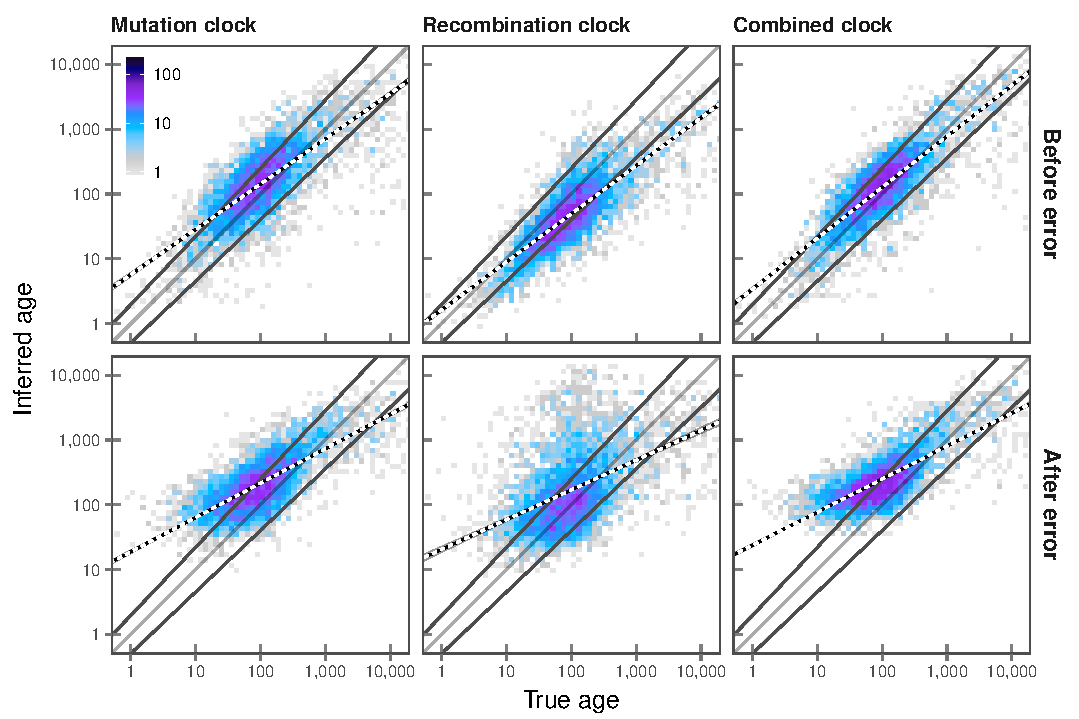
\includegraphics[width=\textwidth]{./img/ch5/generror_scat_fgtH}
{\small\texthv{\textbf{\,(c) FGT, phased haplotypes}}} \\
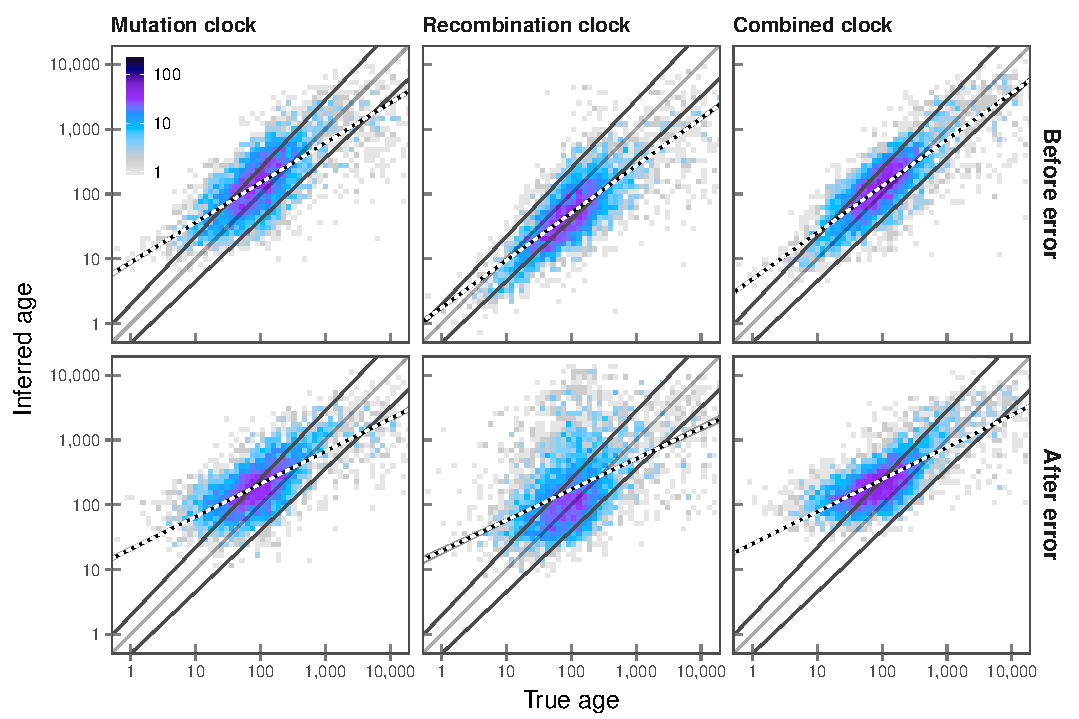
\includegraphics[width=\textwidth]{./img/ch5/generror_scat_fgtP}
\caption[]{Continued.}
\label{fig:generror_scat_fgt}
\end{figure}

%

Before error, \SIlist{53.02094;50.84745;60.03988}{\percent} of alleles were correctly inferred from true haplotype data in \ClockM, \ClockR, and \ClockC, respectively.
When phased data were used, this changed only slightly; \SIlist{50.82752;51.365902;59.18245}{\percent} in \ClockM, \ClockR, and \ClockC, respectively.
Notably, the proportion of correctly inferred alleles increased in \ClockR due to phasing error.
\Correct{It is suggested that} the tendency for underestimation that was generally seen in \ClockR may have been mitigated by further reduction of IBD segment lengths resulting from phasing error.
The small difference between true and phased data was further reflected in $r_S$, which changed from \numrange{0.679635}{0.660366} in \ClockM, \numrange{0.779995}{0.764215} in \ClockR, and \numrange{0.741871}{0.731383} in \ClockC, with regards to $t_d$.

\Correct{After error}, the overall proportion of correct alleles was reduced, but again the differences between true and phased data were small.
On true haplotypes, the proportion of correct alleles was \SIlist{44.26720;45.024925;42.03390}{\percent} in \ClockM, \ClockR, and \ClockC, respectively, whereas \SIlist{43.54935;46.001994;41.63509}{\percent} of alleles were correct using phased haplotypes.
Likewise, $r_S$ and \gls{rmsle} scores did not suggest notable differences between estimation results from true and phased haplotypes; see \cpref{tab:stats_generror}.

\Correct{In the previous analysis using true IBD, it was suggested} that genotype error may induce an overestimation of allele age in \ClockM and \ClockC.
However, this was reduced here,
\Correct{possibly because phasing error may result in truncated shared haplotype intervals, such that shorter intervals may mitigate the effects of data error on observed pairwise differences in a pair haplotypes.}

%
% !TEX root = ../../main.tex


\begin{figure}[tb]
\ContinuedFloat
{\small\texthv{\textbf{\,(d) DGT}}} \\
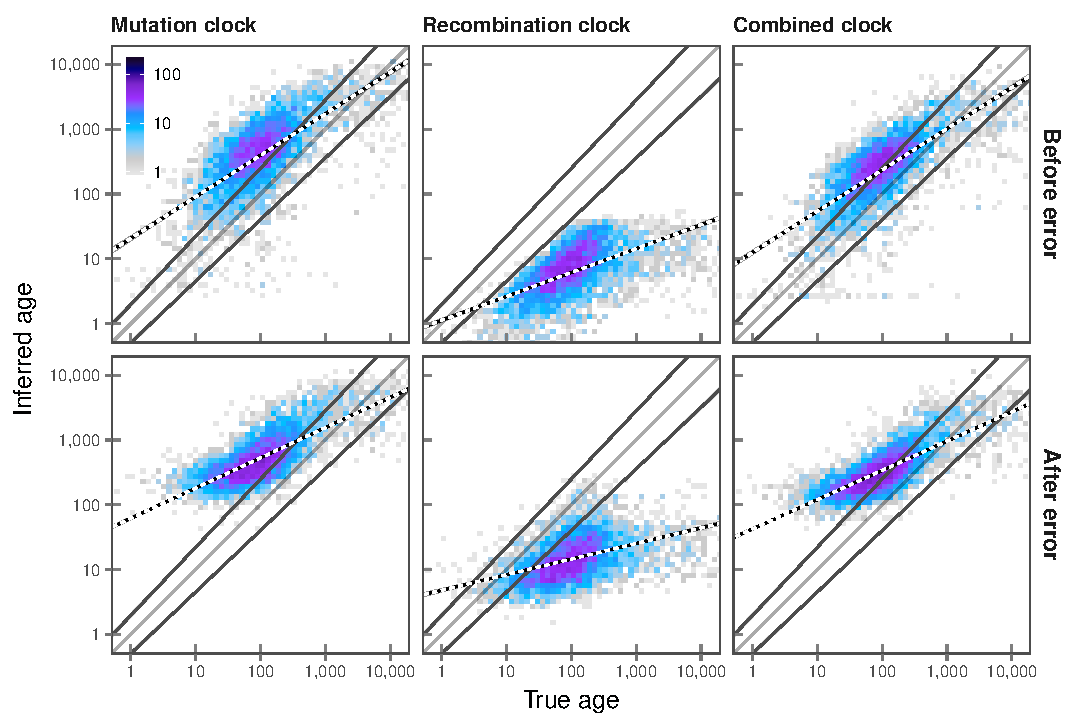
\includegraphics[width=\textwidth]{./img/ch5/generror_scat_dgt}
\caption[]{Continued.}
\label{fig:generror_scat_dgt}
\end{figure}

%

Estimation results based on the \gls{dgt} are shown in \cref{fig:generror_scat_dgt}{d} (\pref{fig:generror_scat_dgt}).
Before error, the proportions of correctly inferred alleles were the lowest in the present comparison in each clock model.
For \ClockM and \ClockC, the estimation resulted in \SIlist{26.34098;36.94915}{\percent} of correct alleles, respectively, whereas only \SI{2.412762}{\percent} were correct for \ClockR.
% While the majority of alleles in \ClockM and \ClockC were overestimated, \SIlist{70.04985;57.84646}{\percent} respectively, \SI{97.58724}{\percent} were underestimated in \ClockR (none were overestimated).
The tendency to overestimate allele age was increased after error.
% The proportions of alleles overestimated were \SIlist{77.30808;67.85643}{\percent} in \ClockM and \ClockC, respectively.
This was also seen for \ClockR, where the proportion of correctly inferred alleles increased to \SI{15.692921}{\percent}, \Correct{but at a loss of accuracy.}
Rank correlation, $r_S$, was \numlist{0.746385;0.627943;0.406151} at $t_c$, $t_m$, and $t_d$ before error, and \numlist{0.588234;0.504469;0.328094} after error; see \cpref{tab:stats_generror}.
% Note that rank correlation at $t_m$ and $t_d$ was higher in \ClockM and \ClockC, both before and after error.
% However, the same measures taken after error actually suggested that the accuracy increased in \ClockM and \ClockC; see .
% Regardless, rank correlation measured at $t_c$ was decreased after error under each clock model.

%
% !TEX root = ../../main.tex


\begin{figure}[tb]
\ContinuedFloat
{\small\texthv{\textbf{\,(e) HMM}}} \\
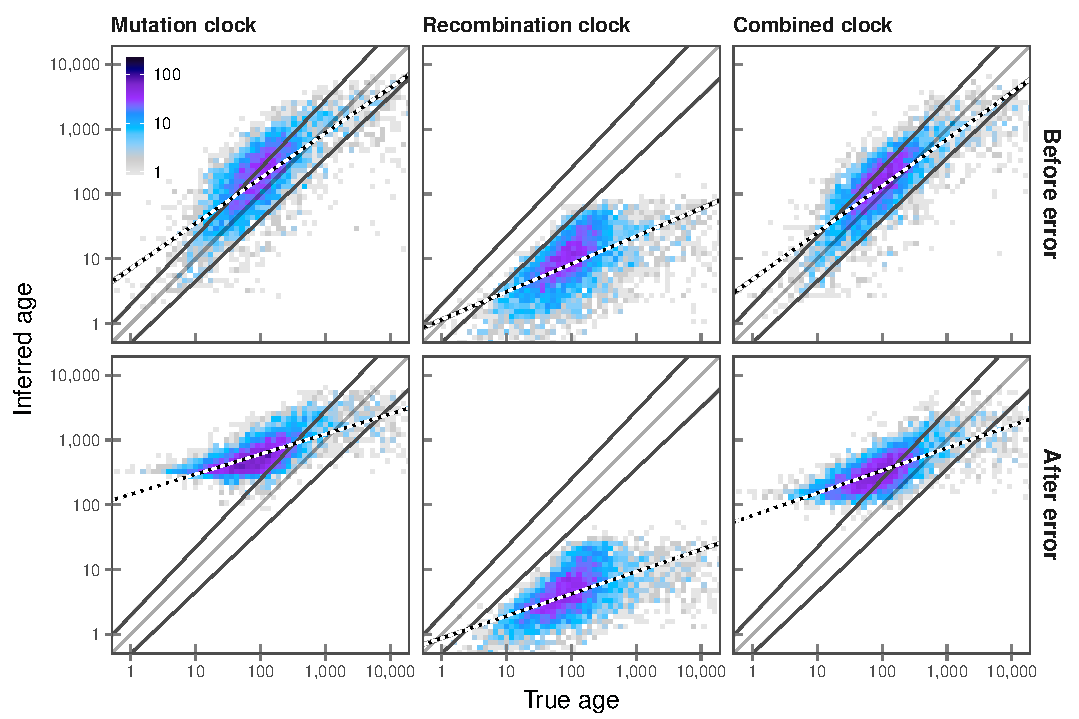
\includegraphics[width=\textwidth]{./img/ch5/generror_scat_hmm}
\caption[]{Continued.}
\label{fig:generror_scat_hmm}
\end{figure}

%

The accuracy of age estimation using the \Correct{genotype-based} \gls{hmm} was relatively high before error; that is, more accurate in comparison to the \gls{fgt} in \ClockM, similar in accuracy to the \gls{dgt} in \ClockR, and similar to the \gls{fgt} in \ClockC.
The density of inferred allele age based on the \gls{hmm} is given in \cref{fig:generror_scat_hmm}{e} (\pref{fig:generror_scat_hmm}).

Before error, the proportion of correct alleles was \SI{47.53739}{\percent} in \ClockM, \SI{3.629113}{\percent} in \ClockR, and \SI{57.82652}{\percent} in \ClockC.
Allele age was generally underestimated in \ClockR (\SI{96.35095}{\percent}).
This was increased after error, resulting in an underestimated proportion of \SI{98.30508}{\percent} in \ClockR, as the proportion of correct alleles was overall reduced; \SIlist{16.65005;27.65703}{\percent} in \ClockM and \ClockC, respectively.
Also, \gls{rmsle} scores were lowest for the \gls{hmm} under each clock model after error; see \cpref{tab:stats_generror}.
\Correct{Rank correlation} before and after error, for $r_S$ at $t_c$, decreased from \dec{0.702418} to \dec{0.534920} in \ClockM, and from \dec{0.733298} to \dec{0.569244} in \ClockC.
Although rank correlation for the \gls{hmm} was high in \ClockR, \eg $r_S$ at $t_c$ was \dec{0.751100} before and \dec{0.737036} after error, \Correct{estimation bias was substantial both before and after error.}
% Although allele age was vastly underestimated, deviations appeared to be consistent.

% %
% % !TEX root = ../../main.tex


\begin{figure}[p]
{\smaller\texthv{\textbf{(a) Before error}}}\\
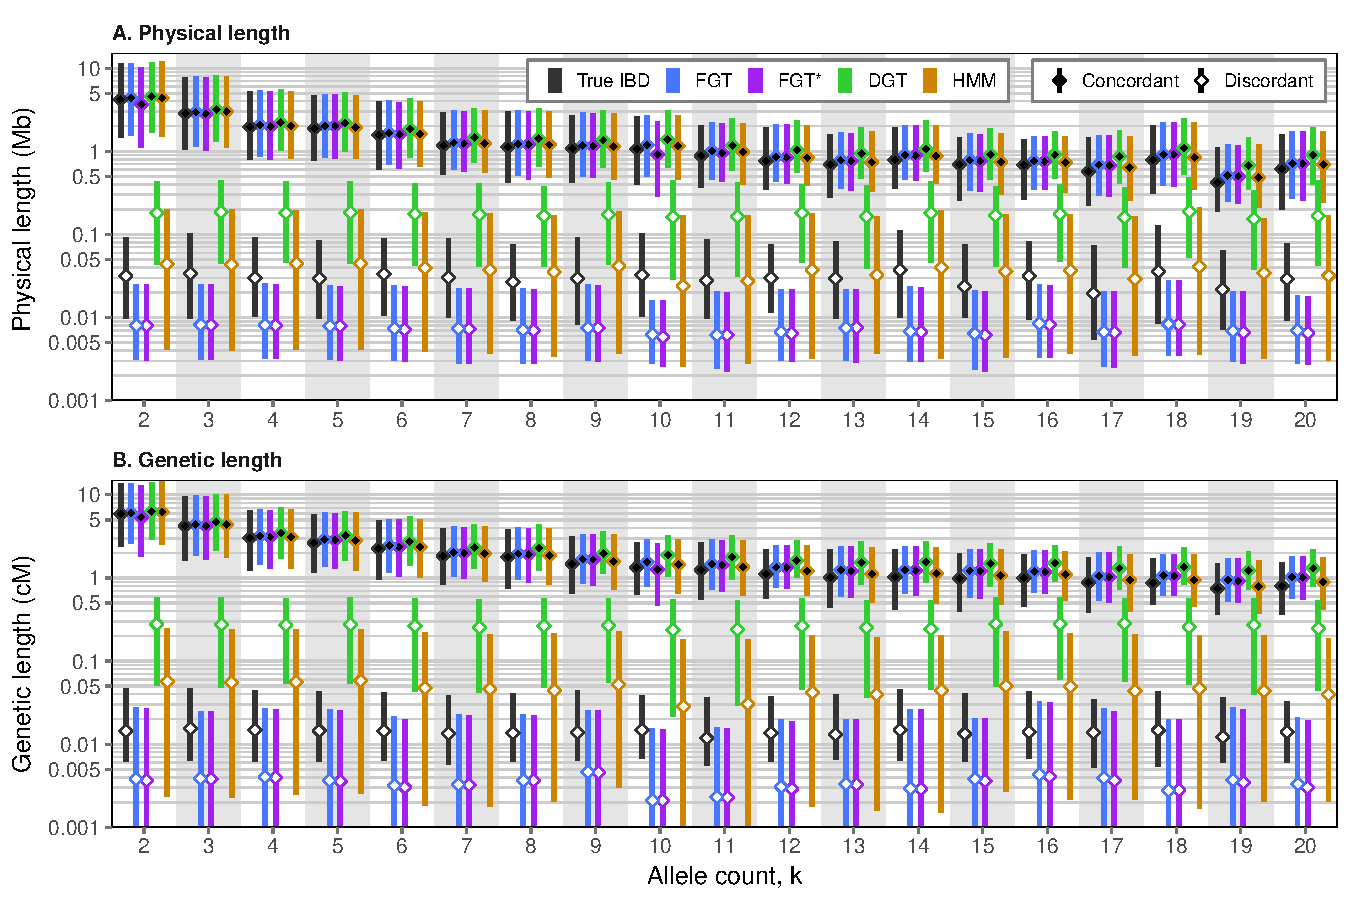
\includegraphics[width=\textwidth]{./img/ch5/africa_length_con_dis_tru}
{\smaller\texthv{\textbf{(b) After error}}}\\
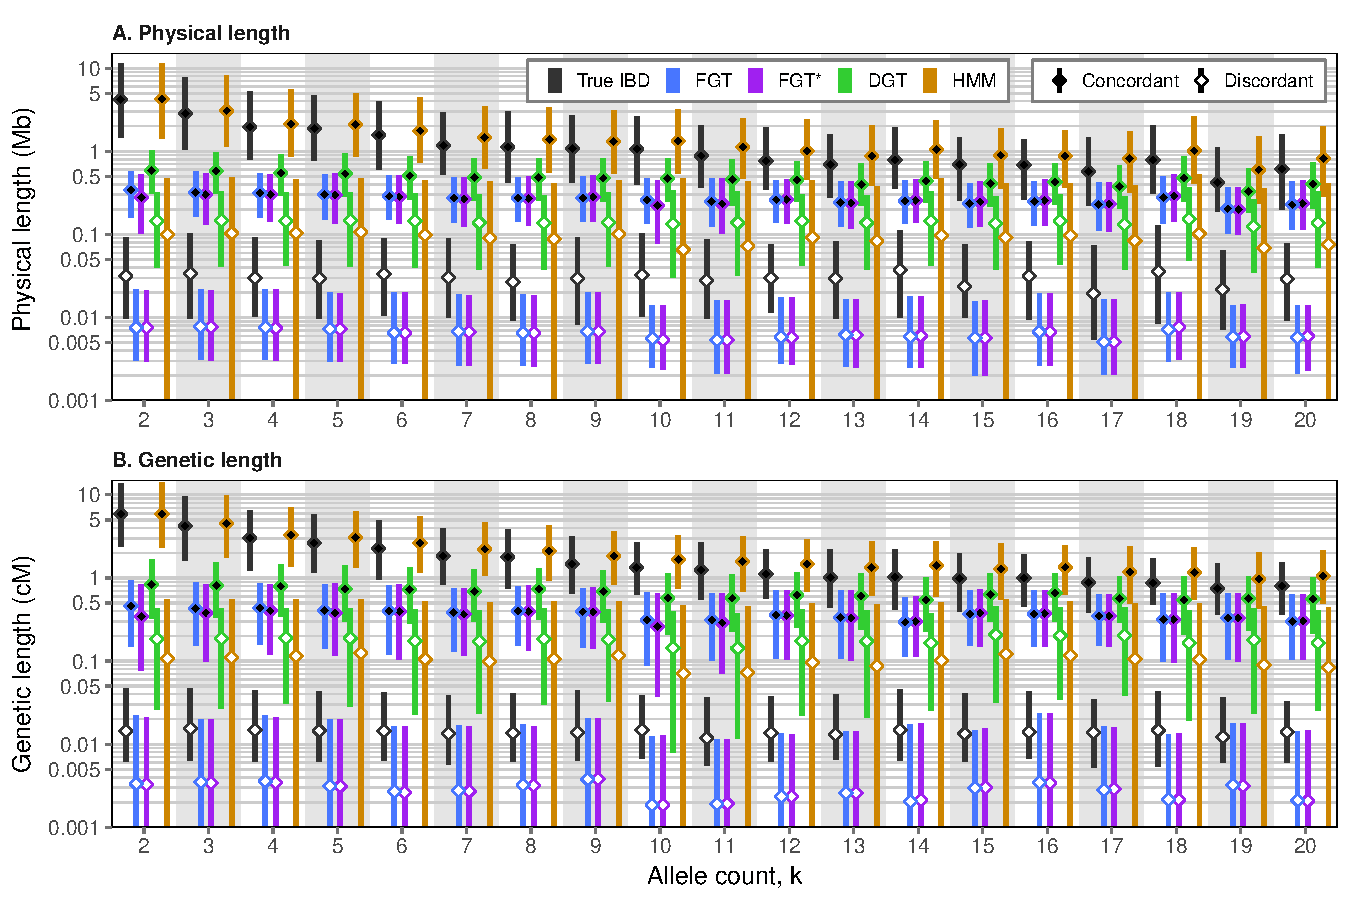
\includegraphics[width=\textwidth]{./img/ch5/africa_length_con_dis_err}
\Caption{Length distribution of inferred IBD segments before and after error}
{Bottom and top of each bar indicate \nth{1} and \nth{3} quartiles, respectively, between which the median (\nth{2} quartile) is marked (\emph{diamonds}).
IBD detected for concordant and discordant pairs is distinguished; \emph{solid} and \emph{hollow} diamonds, respectively.}
{fig:africa_length_con_dis}
\end{figure}

% %
%
% The distribution of inferred IBD segment lengths for each approach are given in \cpref{fig:africa_length_con_dis}.
% Notably, IBD segments detected using the \gls{fgt} and \gls{dgt} were overall underestimated after error; only the HMM maintained similarly accurate lengths before and after error, for both concordant and discordant pairs.


%
% !TEX root = ../../main.tex


\begin{table}[p]
\Caption{Effect of genotype error on age estimation accuracy}
{Allele age was estimated based on IBD inferred using the \gls{fgt}, \gls{dgt}, and \gls{hmm} on the same set of \n{5000} rare allele target sites randomly selected at allele frequency ${\leq 0.5\%}$ (\fk{[2,25]}) in simulated data before and after error (datasets $\mathcal{D}_B$~and~$\mathcal{D}_B^{\ast}$).
The number of discordant pairs was limited to ${n_d = \num{2500}}$ in each analysis.
%Note that the \gls{hmm} used the theoretical emission model in the analysis before error (dataset $\mathcal{D}_B$), and the empirical emission model after error ($\mathcal{D}_B^{\ast}$).
True IBD refers to age estimation conducted using knowledge of the actual shared haplotype structure of the sample, as determined from simulation records.}
{tab:stats_generror}
\centering
\begin{threeparttable}
\begin{tabular}{cl
*3{S[table-format=1.3]}
*3{S[table-format=1.3]}}
\toprule
Clock & Method &
\multicolumn{3}{c}{Before error} &
\multicolumn{3}{c}{After error} \\
\cmidrule(lr){3-5}
\cmidrule(lr){6-8}
& & {$t_c$} & {$t_m$} & {$t_d$} & {$t_c$} & {$t_m$} & {$t_d$} \\
\otoprule
\multicolumn{8}{@{}l}{\,Rank correlation coefficient ($r_S$)} \\
\midrule
\ClockM & {FGT}*             & 0.679635 & 0.735844 & 0.596748  &  0.556029 & 0.696319 & 0.615198   \\
        & {FGT}**            & 0.660366 & 0.711279 & 0.575622  &  0.542974 & 0.673170 & 0.590948  \\
        & {DGT}              & 0.618193 & 0.684883 & 0.563048  &  \bfseries 0.576504 & \bfseries 0.724127 & \bfseries 0.648891   \\
        & {HMM}              & \bfseries 0.702418 & \bfseries 0.737679 & \bfseries 0.598672  &  0.534920 & 0.686005 & 0.620696   \\
				\cmidrule(lr){2-8}
        & \textit{True IBD}  & 0.869553 & 0.870597 & 0.673496  &  0.517705 & 0.694488 & 0.646233   \\
\cmidrule(lr){1-8}
\ClockR & {FGT}*             & \bfseries 0.779995 & \bfseries 0.781699 & 0.600591  &  0.405087 & 0.480883 & 0.407458   \\
        & {FGT}**            & 0.764215 & 0.780367 & \bfseries 0.603175  &  0.405573 & 0.485330 & \bfseries 0.413798   \\
        & {DGT}              & 0.746385 & 0.627943 & 0.406151  &  0.588234 & 0.504469 & 0.328094   \\
        & {HMM}              & 0.751100 & 0.631907 & 0.411213  &  \bfseries 0.737036 & \bfseries 0.621305 & 0.397976   \\
				\cmidrule(lr){2-8}
        & \textit{True IBD}  & 0.818219 & 0.842606 & 0.665742  &  0.818219 & 0.842606 & 0.665742  \\
\cmidrule(lr){1-8}
\ClockC & {FGT}*             & \bfseries 0.741871 & \bfseries 0.791536 & \bfseries 0.644276  &  0.528087 & 0.689074 & 0.629404  \\
        & {FGT}**            & 0.731383 & 0.786636 & 0.642932  &  0.520113 & 0.678718 & 0.619071   \\
        & {DGT}              & 0.666312 & 0.727321 & 0.596733  &  \bfseries 0.596064 & \bfseries 0.756788 & \bfseries 0.688618   \\
        & {HMM}              & 0.733298 & 0.780561 & 0.640797  &  0.569244 & 0.692706 & 0.605695   \\
				\cmidrule(lr){2-8}
        & \textit{True IBD}  & 0.884482 & 0.885414 & 0.695565  &  0.592839 & 0.735099 & 0.654742   \\
\otoprule
\multicolumn{8}{@{}l}{\,\Glsentryfull{rmsle}} \\
\midrule
\ClockM & {FGT}*             & \bfseries 0.695912 & \bfseries 0.435866 & 0.639313  &  0.864236 & \bfseries 0.516007 & \bfseries 0.523529  \\
        & {FGT}**            & 0.714730 & 0.443901 & \bfseries 0.622882  &  \bfseries 0.859224 & 0.523747 & 0.547133  \\
        & {DGT}              & 1.082976 & 0.743112 & 0.657413  &  1.190149 & 0.808980 & 0.605562  \\
        & {HMM}              & 0.753908 & 0.478462 & 0.633496  &  1.249580 & 0.881739 & 0.681390   \\
				\cmidrule(lr){2-8}
        & \textit{True IBD}  & 0.454176 & 0.255423 & 0.665891  &  1.146076 & 0.769767 & 0.586670   \\
\cmidrule(lr){1-8}
\ClockR & {FGT}*             & \bfseries 0.379925 & \bfseries 0.471320 & 0.908926  &  0.881381 & \bfseries 0.638426 & 0.728178   \\
        & {FGT}**            & 0.412751 & 0.479909 & \bfseries 0.902911  &  0.889832 & 0.641047 & \bfseries 0.722131   \\
        & {DGT}              & 0.904773 & 1.251534 & 1.690478  &  \bfseries 0.702780 & 0.991003 & 1.413303   \\
        & {HMM}              & 0.796114 & 1.140817 & 1.584667  &  1.030988 & 1.379900 & 1.814060  \\
				\cmidrule(lr){2-8}
        & \textit{True IBD}  & 0.336637 & 0.503643 & 0.960124  &  0.336637 & 0.503643 & 0.960124   \\
\cmidrule(lr){1-8}
\ClockC & {FGT}*             & \bfseries 0.624316 & \bfseries 0.363891 & 0.626025  &  \bfseries 0.915415 & \bfseries 0.547716 & \bfseries 0.495805   \\
        & {FGT}**            & 0.641259 & 0.367452 & \bfseries 0.607647  &  0.915773 & 0.551215 & 0.502936   \\
        & {DGT}              & 0.869489 & 0.557124 & 0.610704  &  1.019118 & 0.645243 & 0.523330   \\
        & {HMM}              & 0.644401 & 0.398467 & 0.646894  &  1.020843 & 0.672042 & 0.585448   \\
				\cmidrule(lr){2-8}
        & \textit{True IBD}  & 0.381267 & 0.260169 & 0.716084  &  0.918903 & 0.555312 & 0.505697  \\
\bottomrule
\end{tabular}
\begin{tablenotes}\footnotesize
	\item[{${\ast}$}] ~ FGT applied to true haplotypes
	\item[{${\ast\ast}$}] ~ FGT applied to phased haplotypes
\end{tablenotes}
\end{threeparttable}
\end{table}


%
% Removed "correction model"
%
%
% \midrule
% \ClockM & {FGT}*             & 0.679635 & 0.735844 & 0.596748  &  0.556029 & 0.696319 & 0.615198  &  0.612817 & 0.721463 & 0.606704 \\
%         & {FGT}**            & 0.660366 & 0.711279 & 0.575622  &  0.542974 & 0.673170 & 0.590948  &  0.597249 & 0.696299 & 0.582121 \\
%         & {DGT}              & 0.618193 & 0.684883 & 0.563048  &  \bfseries 0.576504 & \bfseries 0.724127 & \bfseries 0.648891  &  0.668763 & \bfseries 0.752897 & \bfseries 0.620062 \\
%         & {HMM}              & \bfseries 0.702418 & \bfseries 0.737679 & \bfseries 0.598672  &  0.534920 & 0.686005 & 0.620696  &  \bfseries 0.675628 & 0.715205 & 0.563232 \\
% 				\cmidrule(lr){2-11}
%         & \textit{True IBD}  & 0.869553 & 0.870597 & 0.673496  &  0.517705 & 0.694488 & 0.646233  &  0.712187 & 0.752078 & 0.589713 \\
% \cmidrule(lr){1-11}
% \ClockR & {FGT}*             & \bfseries 0.779995 & \bfseries 0.781699 & 0.600591  &  0.405087 & 0.480883 & 0.407458  &  0.462489 & 0.515341 & 0.414202 \\
%         & {FGT}**            & 0.764215 & 0.780367 & \bfseries 0.603175  &  0.405573 & 0.485330 & \bfseries 0.413798  &  0.461183 & 0.518974 & \bfseries 0.420213 \\
%         & {DGT}              & 0.746385 & 0.627943 & 0.406151  &  0.588234 & 0.504469 & 0.328094  &  0.629528 & 0.530195 & 0.335903 \\
%         & {HMM}              & 0.751100 & 0.631907 & 0.411213  &  \bfseries 0.737036 & \bfseries 0.621305 & 0.397976  &  \bfseries 0.737611 & \bfseries 0.624484 & 0.402304 \\
% 				\cmidrule(lr){2-11}
%         & \textit{True IBD}  & 0.818219 & 0.842606 & 0.665742  &  0.818219 & 0.842606 & 0.665742  &  0.801053 & 0.848582 & 0.684321 \\
% \cmidrule(lr){1-11}
% \ClockC & {FGT}*             & \bfseries 0.741871 & \bfseries 0.791536 & \bfseries 0.644276  &  0.528087 & 0.689074 & 0.629404  &  0.640146 & 0.741473 & 0.617204 \\
%         & {FGT}**            & 0.731383 & 0.786636 & 0.642932  &  0.520113 & 0.678718 & 0.619071  &  0.630920 & 0.731960 & 0.608941 \\
%         & {DGT}              & 0.666312 & 0.727321 & 0.596733  &  \bfseries 0.596064 & \bfseries 0.756788 & \bfseries 0.688618  &  \bfseries 0.694033 & \bfseries 0.780836 & \bfseries 0.645128 \\
%         & {HMM}              & 0.733298 & 0.780561 & 0.640797  &  0.569244 & 0.692706 & 0.605695  &  0.678579 & 0.718316 & 0.567673 \\
% 				\cmidrule(lr){2-11}
%         & \textit{True IBD}  & 0.884482 & 0.885414 & 0.695565  &  0.592839 & 0.735099 & 0.654742  &  0.740229 & 0.777507 & 0.612734 \\
% \otoprule
% \multicolumn{11}{@{}l}{\,\Glsentryfull{rmsle}} \\
% \midrule
% \ClockM & {FGT}*             & \bfseries 0.695912 & \bfseries 0.435866 & 0.639313  &  0.864236 & \bfseries 0.516007 & \bfseries 0.523529  &  0.614739 & 0.394410 & \bfseries 0.661791 \\
%         & {FGT}**            & 0.714730 & 0.443901 & \bfseries 0.622882  &  \bfseries 0.859224 & 0.523747 & 0.547133  &  0.625120 & 0.415860 & 0.678010 \\
%         & {DGT}              & 1.082976 & 0.743112 & 0.657413  &  1.190149 & 0.808980 & 0.605562  &  \bfseries 0.592894 & \bfseries 0.382332 & 0.667709 \\
%         & {HMM}              & 0.753908 & 0.478462 & 0.633496  &  1.249580 & 0.881739 & 0.681390  &  0.597727 & 0.424612 & 0.713284 \\
% 				\cmidrule(lr){2-11}
%         & \textit{True IBD}  & 0.454176 & 0.255423 & 0.665891  &  1.146076 & 0.769767 & 0.586670  &  0.562468 & 0.362053 & 0.671419 \\
% \cmidrule(lr){1-11}
% \ClockR & {FGT}*             & \bfseries 0.379925 & \bfseries 0.471320 & 0.908926  &  0.881381 & \bfseries 0.638426 & 0.728178  &  0.738054 & 0.593683 & 0.815015 \\
%         & {FGT}**            & 0.412751 & 0.479909 & \bfseries 0.902911  &  0.889832 & 0.641047 & \bfseries 0.722131  &  0.742086 & 0.593570 & 0.811059 \\
%         & {DGT}              & 0.904773 & 1.251534 & 1.690478  &  \bfseries 0.702780 & 0.991003 & 1.413303  &  0.630794 & 0.532640 & 0.821584 \\
%         & {HMM}              & 0.796114 & 1.140817 & 1.584667  &  1.030988 & 1.379900 & 1.814060  &  \bfseries 0.590344 & \bfseries 0.487898 & \bfseries 0.797895 \\
% 				\cmidrule(lr){2-11}
%         & \textit{True IBD}  & 0.336637 & 0.503643 & 0.960124  &  0.336637 & 0.503643 & 0.960124  &  0.507989 & 0.283677 & 0.645182 \\
% \cmidrule(lr){1-11}
% \ClockC & {FGT}*             & \bfseries 0.624316 & \bfseries 0.363891 & 0.626025  &  \bfseries 0.915415 & \bfseries 0.547716 & \bfseries 0.495805  &  0.601021 & 0.372863 & \bfseries 0.649076 \\
%         & {FGT}**            & 0.641259 & 0.367452 & \bfseries 0.607647  &  0.915773 & 0.551215 & 0.502936  &  0.608757 & 0.383502 & 0.654150 \\
%         & {DGT}              & 0.869489 & 0.557124 & 0.610704  &  1.019118 & 0.645243 & 0.523330  &  \bfseries 0.587156 & \bfseries 0.372073 & 0.661028 \\
%         & {HMM}              & 0.644401 & 0.398467 & 0.646894  &  1.020843 & 0.672042 & 0.585448  &  0.595058 & 0.420826 & 0.711664 \\
% 				\cmidrule(lr){2-11}
%         & \textit{True IBD}  & 0.381267 & 0.260169 & 0.716084  &  0.918903 & 0.555312 & 0.505697  &  0.541655 & 0.330076 & 0.656368 \\
% \bottomrule

%




%
\subsection{Discussion}
%


% method to narrow down discordant pairs by finding nearest neighbours in outgroup

% outlier identification; inferred IBD lengths that appear to deviate markedly from lengths detected for other pairs that share the same focal allele; separately for concordant and discordant pairs

I demonstrated the validity of the age estimation framework using simulated data where I showed that age can be estimated with very high accuracy.
However, certain problems may arise when working with real data.
Notably, ihe impact of phasing error is small in comparison to genotypic (or allelic) misclassification, which is likely to bias the estimation process.

Generally, imperfect data may affect the estimation of allele age in \n{2} ways.
First, the method was shown to be highly susceptible to inaccurate IBD inference, where each clock model behaves differently to the over or underestimation of IBD length.
% In this regard, the \gls{hmm}-based approach for IBD inference was shown to maintain consistency even if genotype error is present.
However, second, \Correct{even for a method that can infer shared haplotype segments} with high accuracy, the alleles observed at a focal site in the sample may wrongly identify haplotype sharing.
To account for the possibility that some concordant pairs may actually be discordant pairs (or \emph{vice versa}), for example, a separate filtering method would be needed to exclude pairs based on patterns of the inferred haplotype structure.
But because such a method would effectively predict falsely called or typed alleles in the data, a solution to this problem may not be straightforward.
% Yet it would be possible, for example, to exclude pairs on basis of patterns of allele sharing or consistency of the inferred IBD structure.
% Alternatively, instead of excluding pairs, the target site itself would need to be excluded from the analysis if bias is likely.
% A simple solution was presented in the previous section, where sites are excluded if the lower and upper bounds indicate a reverse order, but further evaluation is required to determine the effectiveness of this filtering criterion.

% Lastly, note that both the \gls{dgt} and the \gls{hmm}-based approach operate on genotype data to detect IBD, but because the mutation clock model, \ClockM, requires haplotypes, it would be desirable to estimate pairwise differences in genotype data, so as to make these methods fully compatible with \ClockM and \ClockC.
% A possible solution is presented in Chapter~3, where haplotype phase was determined from genotype pairs in detected IBD segments, based on the genealogical constrains that arise under haplotype sharing by descent.
% Yet, further work is needed to determine the feasibility of such an approach.

\Addition{In conclusion, a substantial amount of estimation bias was seen for any of the evaluated methods for shared haplotype inference.
Due to the dependency on finding genuine haplotype intervals, the allele age estimation method may therefore not be regarded as being reliable in applications to real data.
However, a solution is attempted in the following section, where I present a novel haplotype-based \gls{hmm} as an advancement over of the current genotype-based method.}


\DeleteNote{Section ``Generation of error correction models''}


\DeleteNote{Section ``Age of alleles with predicted effects in 1000 Genomes data''}













%
% Text below was replaced to make space for new results
%
%
% %
% \subsubsection{Generation of error correction models}
% \label{sec:age_corrfactor}
% %
%
% Although the estimation showed strong tendencies to either over- or underestimate allele age, dependent on the clock model and IBD method used, some settings maintained relatively high levels of accuracy after error; in particular the \gls{hmm}-based inference in \ClockR.
% This suggested that deviations from the true age may follow a consistent pattern.
% As it is hoped that the age estimation method presented in this chapter is able to produce credible results when used on real data, I evaluated the reliability of each estimation approach by constructing error correction models specific to each setting.
%
% The deviation of the estimated age, $\hat{t}$, from the actual true age of an allele, denoted by $t^\ast$, is simply the absolute value of their difference; calculated as ${\delta = | \hat{t} - t^\ast |}$.
% Given the expectation that the time to coalescence is exponentially distributed, the logarithmic difference is calculated as
% \begin{equation}
% 	\xi ~=~ \frac{t^\ast \euler{-\delta}}{\hat{t}}
% \end{equation}
% where ${\xi = 0}$ if true and estimated age are equal, ${0 < \xi < 1}$ if the age is overestimated, and ${\xi > 1}$ if age is underestimated.
% As the actual age of an allele was not known from coalescent simulations, here, the midpoint of the branch on which the mutation event occurred, $t_m$, was defined as the reference point against which the estimated age was compared.
% In reverse, a constant $\xi$ value was used as a correction factor applied to a given set of analysed alleles, considering the results obtained per clock model and IBD method, in order to minimise the mean of the difference distribution.
% The value of this correction factor was estimated by iteration through an array, denoted by $\Xi$, which is defined as a series of $l$ factor values, denoted by ${\xi_i \in \Xi}$, where ${i \in [ 1, 2, \ldots l]}$.
% The minimum factor value was found through the following operation;
% \begin{equation}\label{eq:corrfactorcalc}
% 	i = \argmin_{\xi_i ~\in~ \Xi} \left( \bigg| ~ \frac{1}{n} \sum_{j=1}^n \log \big[ {t_m}_j \big] - \log \big[ \hat{t}_j ~ \xi_i \big] ~ \bigg| \right)
% \end{equation}
% which is applied to a given set of $n$ true and corresponding estimated times, ${t_m}_j$ and ${\hat{t}_j}$, respectively, where ${j \in 1, 2, \ldots, n}$.
% I applied \cref{eq:corrfactorcalc} in a recursive algorithm in which I selected $\xi_{i-1}$ and $\xi_{i+1}$ after each step to redefine the limits of $\Xi$ and to recalculate $l$ new factor values for the next step.
% This greatly improved the speed and resolution of the computation.
%
% %
% % !TEX root = ../../main.tex


\begin{figure}[!htb]
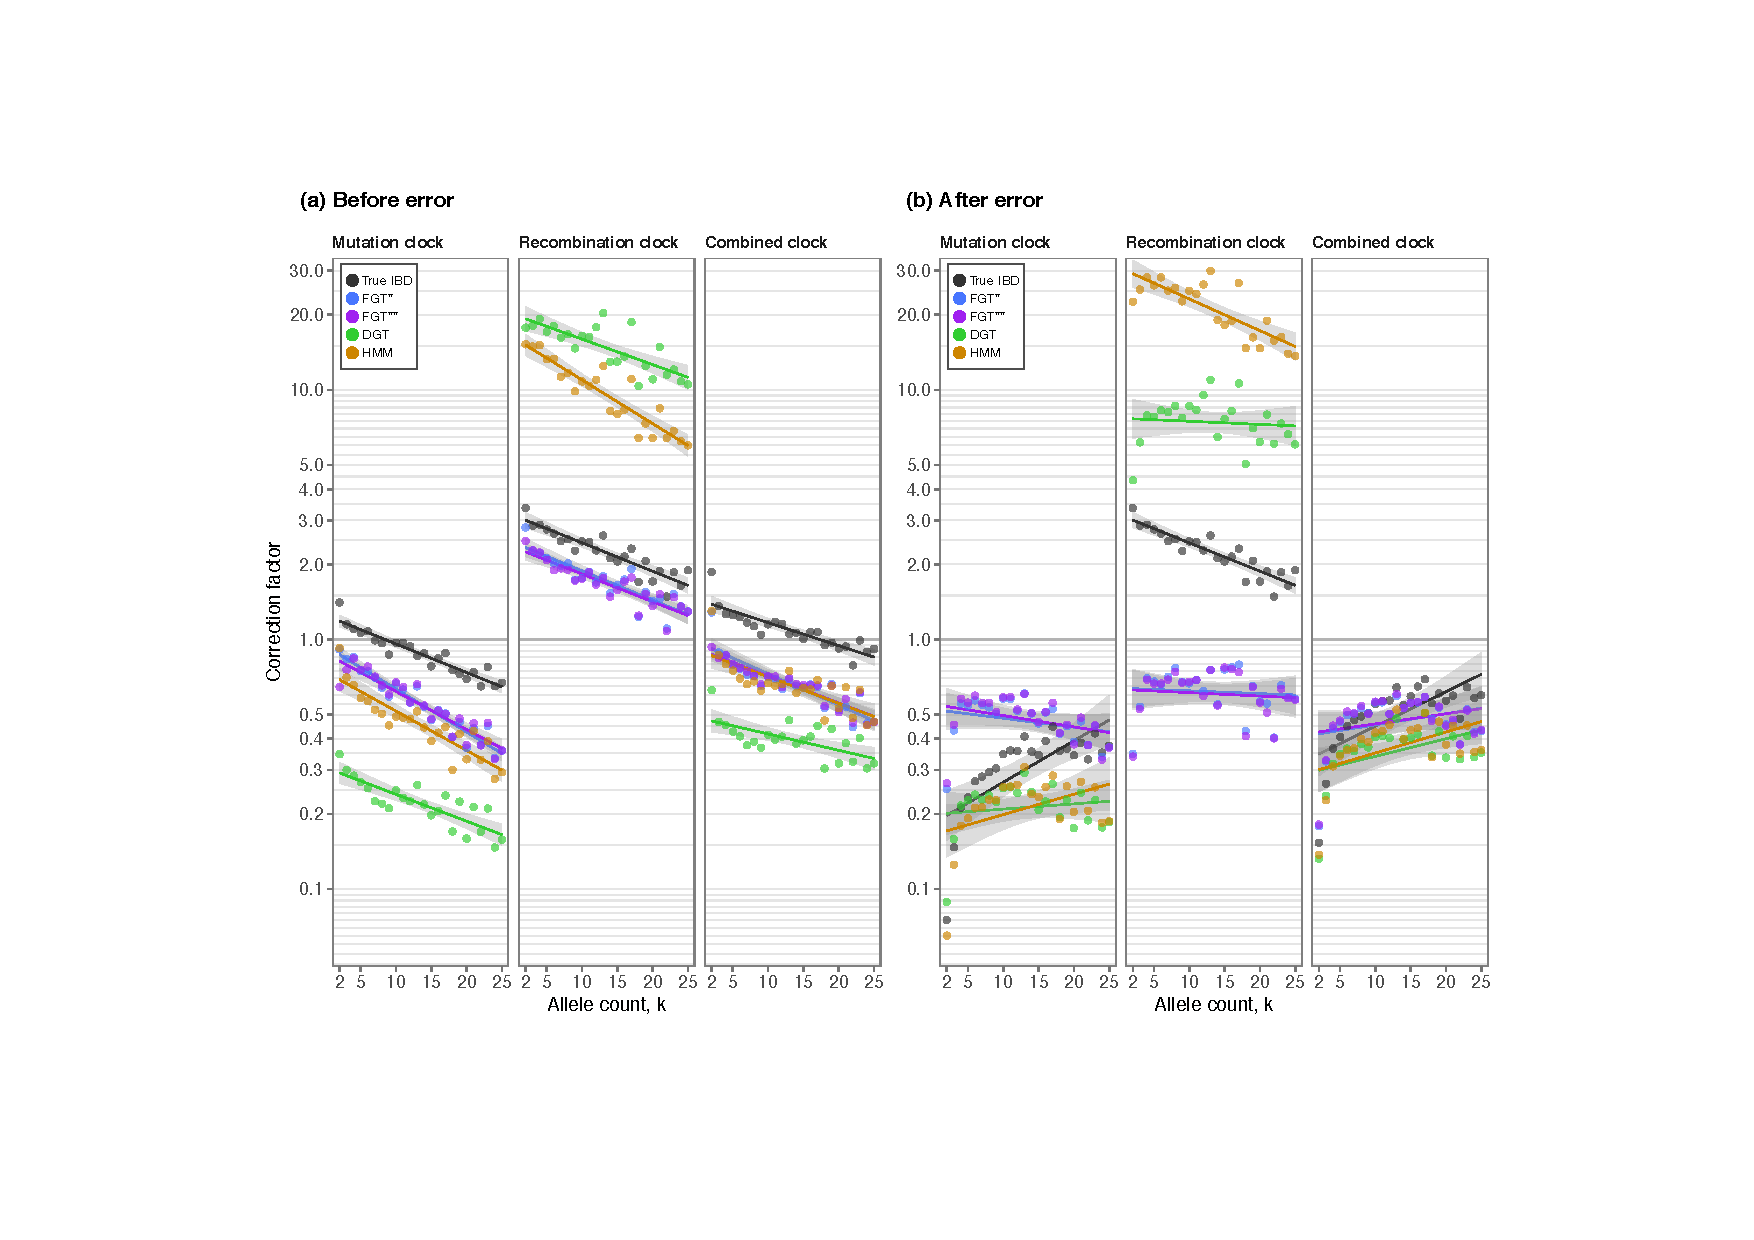
\includegraphics[width=\textwidth]{./img/ch5/generror_factor}
\Caption{Estimated correction factors before and after error}
{Correction factors were estimated per set of \fk{}~variants for which allele age was estimated in each analysis under a given clock model and IBD detection method.
Values below and above 1 indicate that true age was overestimated and underestimated on average, respectively.
The line shown per analysis indicates the trend of the corrected deviation ($\pm\,\text{SE}$), which was calculated through simple nonlinear regression by allele frequency.
Note that IBD detection using the \gls{fgt} was performed on true haplotype data (*) as well as phased haplotypes (**).}
{fig:generror_factor}
\end{figure}

% %
%
% The algorithm outlined above was applied on the results obtained per set of \fk{}~variants estimated in each clock model and IBD method, as well as true IBD, before and after error.
% Computed correction factors are shown in \cref{fig:generror_factor}, which highlights that deviations followed a general trend in each analysis.
% For example, before error, allele age estimated using true IBD showed the lowest amount of deviation in \ClockM and \ClockC, but where alleles at lower frequencies showed a tendency to be overestimated on average and underestimated at higher frequencies.
% However, in \ClockR, true IBD showed larger deviations compared to the \gls{fgt} (on both true and phased haplotype data), but this may result from the assumption that $t_m$ approximates the actual age of an allele.
% After error, notably, factor deviations showed spurious patterns for most approaches, except for the \gls{hmm}-based estimation of allele age, which indicated a consistent trend.
% Note that the factor distributions of true IBD in \ClockR were identical before and after error, as genotype error did not affect the estimation under the recombination clock when IBD is known.
%
% Generated error correction factors were applied to the estimated age results, after error, at corresponding \fk{}~variants under each clock model and in each IBD method, which minimised deviations in relation to $t_m$.
% As a consequence, accuracy was overall improved in each approach; see \cpref{tab:stats_generror}.
% Notably, however, the rank correlation measured for the \gls{hmm} in \ClockR was least affected; before applying correction factors, $r_S$ was \numlist{0.737036;0.621305;0.397976} at  $t_c$, $t_m$, and $t_d$, respectively, which was marginally improved after correction, yielding \numlist{0.737611;0.624484;0.402304}, respectively.
% Nonetheless, the \gls{hmm} indicated the highest levels of accuracy at these measures in comparison to the other IBD methods.
% Hence, this result corroborates the reliability of the \gls{hmm} in \ClockR.
%
% %
% % !TEX root = ../../main.tex


\begin{table}[p]
\Caption{Effect of genotype error on age estimation accuracy}
{Allele age was estimated based on IBD inferred using the \gls{fgt}, \gls{dgt}, and \gls{hmm} on the same set of \n{5000} rare allele target sites randomly selected at allele frequency ${\leq 0.5\%}$ (\fk{[2,25]}) in simulated data before and after error (datasets $\mathcal{D}_B$~and~$\mathcal{D}_B^{\ast}$).
The number of discordant pairs was limited to ${n_d = \num{2500}}$ in each analysis.
%Note that the \gls{hmm} used the theoretical emission model in the analysis before error (dataset $\mathcal{D}_B$), and the empirical emission model after error ($\mathcal{D}_B^{\ast}$).
True IBD refers to age estimation conducted using knowledge of the actual shared haplotype structure of the sample, as determined from simulation records.}
{tab:stats_generror}
\centering
\begin{threeparttable}
\begin{tabular}{cl
*3{S[table-format=1.3]}
*3{S[table-format=1.3]}}
\toprule
Clock & Method &
\multicolumn{3}{c}{Before error} &
\multicolumn{3}{c}{After error} \\
\cmidrule(lr){3-5}
\cmidrule(lr){6-8}
& & {$t_c$} & {$t_m$} & {$t_d$} & {$t_c$} & {$t_m$} & {$t_d$} \\
\otoprule
\multicolumn{8}{@{}l}{\,Rank correlation coefficient ($r_S$)} \\
\midrule
\ClockM & {FGT}*             & 0.679635 & 0.735844 & 0.596748  &  0.556029 & 0.696319 & 0.615198   \\
        & {FGT}**            & 0.660366 & 0.711279 & 0.575622  &  0.542974 & 0.673170 & 0.590948  \\
        & {DGT}              & 0.618193 & 0.684883 & 0.563048  &  \bfseries 0.576504 & \bfseries 0.724127 & \bfseries 0.648891   \\
        & {HMM}              & \bfseries 0.702418 & \bfseries 0.737679 & \bfseries 0.598672  &  0.534920 & 0.686005 & 0.620696   \\
				\cmidrule(lr){2-8}
        & \textit{True IBD}  & 0.869553 & 0.870597 & 0.673496  &  0.517705 & 0.694488 & 0.646233   \\
\cmidrule(lr){1-8}
\ClockR & {FGT}*             & \bfseries 0.779995 & \bfseries 0.781699 & 0.600591  &  0.405087 & 0.480883 & 0.407458   \\
        & {FGT}**            & 0.764215 & 0.780367 & \bfseries 0.603175  &  0.405573 & 0.485330 & \bfseries 0.413798   \\
        & {DGT}              & 0.746385 & 0.627943 & 0.406151  &  0.588234 & 0.504469 & 0.328094   \\
        & {HMM}              & 0.751100 & 0.631907 & 0.411213  &  \bfseries 0.737036 & \bfseries 0.621305 & 0.397976   \\
				\cmidrule(lr){2-8}
        & \textit{True IBD}  & 0.818219 & 0.842606 & 0.665742  &  0.818219 & 0.842606 & 0.665742  \\
\cmidrule(lr){1-8}
\ClockC & {FGT}*             & \bfseries 0.741871 & \bfseries 0.791536 & \bfseries 0.644276  &  0.528087 & 0.689074 & 0.629404  \\
        & {FGT}**            & 0.731383 & 0.786636 & 0.642932  &  0.520113 & 0.678718 & 0.619071   \\
        & {DGT}              & 0.666312 & 0.727321 & 0.596733  &  \bfseries 0.596064 & \bfseries 0.756788 & \bfseries 0.688618   \\
        & {HMM}              & 0.733298 & 0.780561 & 0.640797  &  0.569244 & 0.692706 & 0.605695   \\
				\cmidrule(lr){2-8}
        & \textit{True IBD}  & 0.884482 & 0.885414 & 0.695565  &  0.592839 & 0.735099 & 0.654742   \\
\otoprule
\multicolumn{8}{@{}l}{\,\Glsentryfull{rmsle}} \\
\midrule
\ClockM & {FGT}*             & \bfseries 0.695912 & \bfseries 0.435866 & 0.639313  &  0.864236 & \bfseries 0.516007 & \bfseries 0.523529  \\
        & {FGT}**            & 0.714730 & 0.443901 & \bfseries 0.622882  &  \bfseries 0.859224 & 0.523747 & 0.547133  \\
        & {DGT}              & 1.082976 & 0.743112 & 0.657413  &  1.190149 & 0.808980 & 0.605562  \\
        & {HMM}              & 0.753908 & 0.478462 & 0.633496  &  1.249580 & 0.881739 & 0.681390   \\
				\cmidrule(lr){2-8}
        & \textit{True IBD}  & 0.454176 & 0.255423 & 0.665891  &  1.146076 & 0.769767 & 0.586670   \\
\cmidrule(lr){1-8}
\ClockR & {FGT}*             & \bfseries 0.379925 & \bfseries 0.471320 & 0.908926  &  0.881381 & \bfseries 0.638426 & 0.728178   \\
        & {FGT}**            & 0.412751 & 0.479909 & \bfseries 0.902911  &  0.889832 & 0.641047 & \bfseries 0.722131   \\
        & {DGT}              & 0.904773 & 1.251534 & 1.690478  &  \bfseries 0.702780 & 0.991003 & 1.413303   \\
        & {HMM}              & 0.796114 & 1.140817 & 1.584667  &  1.030988 & 1.379900 & 1.814060  \\
				\cmidrule(lr){2-8}
        & \textit{True IBD}  & 0.336637 & 0.503643 & 0.960124  &  0.336637 & 0.503643 & 0.960124   \\
\cmidrule(lr){1-8}
\ClockC & {FGT}*             & \bfseries 0.624316 & \bfseries 0.363891 & 0.626025  &  \bfseries 0.915415 & \bfseries 0.547716 & \bfseries 0.495805   \\
        & {FGT}**            & 0.641259 & 0.367452 & \bfseries 0.607647  &  0.915773 & 0.551215 & 0.502936   \\
        & {DGT}              & 0.869489 & 0.557124 & 0.610704  &  1.019118 & 0.645243 & 0.523330   \\
        & {HMM}              & 0.644401 & 0.398467 & 0.646894  &  1.020843 & 0.672042 & 0.585448   \\
				\cmidrule(lr){2-8}
        & \textit{True IBD}  & 0.381267 & 0.260169 & 0.716084  &  0.918903 & 0.555312 & 0.505697  \\
\bottomrule
\end{tabular}
\begin{tablenotes}\footnotesize
	\item[{${\ast}$}] ~ FGT applied to true haplotypes
	\item[{${\ast\ast}$}] ~ FGT applied to phased haplotypes
\end{tablenotes}
\end{threeparttable}
\end{table}


%
% Removed "correction model"
%
%
% \midrule
% \ClockM & {FGT}*             & 0.679635 & 0.735844 & 0.596748  &  0.556029 & 0.696319 & 0.615198  &  0.612817 & 0.721463 & 0.606704 \\
%         & {FGT}**            & 0.660366 & 0.711279 & 0.575622  &  0.542974 & 0.673170 & 0.590948  &  0.597249 & 0.696299 & 0.582121 \\
%         & {DGT}              & 0.618193 & 0.684883 & 0.563048  &  \bfseries 0.576504 & \bfseries 0.724127 & \bfseries 0.648891  &  0.668763 & \bfseries 0.752897 & \bfseries 0.620062 \\
%         & {HMM}              & \bfseries 0.702418 & \bfseries 0.737679 & \bfseries 0.598672  &  0.534920 & 0.686005 & 0.620696  &  \bfseries 0.675628 & 0.715205 & 0.563232 \\
% 				\cmidrule(lr){2-11}
%         & \textit{True IBD}  & 0.869553 & 0.870597 & 0.673496  &  0.517705 & 0.694488 & 0.646233  &  0.712187 & 0.752078 & 0.589713 \\
% \cmidrule(lr){1-11}
% \ClockR & {FGT}*             & \bfseries 0.779995 & \bfseries 0.781699 & 0.600591  &  0.405087 & 0.480883 & 0.407458  &  0.462489 & 0.515341 & 0.414202 \\
%         & {FGT}**            & 0.764215 & 0.780367 & \bfseries 0.603175  &  0.405573 & 0.485330 & \bfseries 0.413798  &  0.461183 & 0.518974 & \bfseries 0.420213 \\
%         & {DGT}              & 0.746385 & 0.627943 & 0.406151  &  0.588234 & 0.504469 & 0.328094  &  0.629528 & 0.530195 & 0.335903 \\
%         & {HMM}              & 0.751100 & 0.631907 & 0.411213  &  \bfseries 0.737036 & \bfseries 0.621305 & 0.397976  &  \bfseries 0.737611 & \bfseries 0.624484 & 0.402304 \\
% 				\cmidrule(lr){2-11}
%         & \textit{True IBD}  & 0.818219 & 0.842606 & 0.665742  &  0.818219 & 0.842606 & 0.665742  &  0.801053 & 0.848582 & 0.684321 \\
% \cmidrule(lr){1-11}
% \ClockC & {FGT}*             & \bfseries 0.741871 & \bfseries 0.791536 & \bfseries 0.644276  &  0.528087 & 0.689074 & 0.629404  &  0.640146 & 0.741473 & 0.617204 \\
%         & {FGT}**            & 0.731383 & 0.786636 & 0.642932  &  0.520113 & 0.678718 & 0.619071  &  0.630920 & 0.731960 & 0.608941 \\
%         & {DGT}              & 0.666312 & 0.727321 & 0.596733  &  \bfseries 0.596064 & \bfseries 0.756788 & \bfseries 0.688618  &  \bfseries 0.694033 & \bfseries 0.780836 & \bfseries 0.645128 \\
%         & {HMM}              & 0.733298 & 0.780561 & 0.640797  &  0.569244 & 0.692706 & 0.605695  &  0.678579 & 0.718316 & 0.567673 \\
% 				\cmidrule(lr){2-11}
%         & \textit{True IBD}  & 0.884482 & 0.885414 & 0.695565  &  0.592839 & 0.735099 & 0.654742  &  0.740229 & 0.777507 & 0.612734 \\
% \otoprule
% \multicolumn{11}{@{}l}{\,\Glsentryfull{rmsle}} \\
% \midrule
% \ClockM & {FGT}*             & \bfseries 0.695912 & \bfseries 0.435866 & 0.639313  &  0.864236 & \bfseries 0.516007 & \bfseries 0.523529  &  0.614739 & 0.394410 & \bfseries 0.661791 \\
%         & {FGT}**            & 0.714730 & 0.443901 & \bfseries 0.622882  &  \bfseries 0.859224 & 0.523747 & 0.547133  &  0.625120 & 0.415860 & 0.678010 \\
%         & {DGT}              & 1.082976 & 0.743112 & 0.657413  &  1.190149 & 0.808980 & 0.605562  &  \bfseries 0.592894 & \bfseries 0.382332 & 0.667709 \\
%         & {HMM}              & 0.753908 & 0.478462 & 0.633496  &  1.249580 & 0.881739 & 0.681390  &  0.597727 & 0.424612 & 0.713284 \\
% 				\cmidrule(lr){2-11}
%         & \textit{True IBD}  & 0.454176 & 0.255423 & 0.665891  &  1.146076 & 0.769767 & 0.586670  &  0.562468 & 0.362053 & 0.671419 \\
% \cmidrule(lr){1-11}
% \ClockR & {FGT}*             & \bfseries 0.379925 & \bfseries 0.471320 & 0.908926  &  0.881381 & \bfseries 0.638426 & 0.728178  &  0.738054 & 0.593683 & 0.815015 \\
%         & {FGT}**            & 0.412751 & 0.479909 & \bfseries 0.902911  &  0.889832 & 0.641047 & \bfseries 0.722131  &  0.742086 & 0.593570 & 0.811059 \\
%         & {DGT}              & 0.904773 & 1.251534 & 1.690478  &  \bfseries 0.702780 & 0.991003 & 1.413303  &  0.630794 & 0.532640 & 0.821584 \\
%         & {HMM}              & 0.796114 & 1.140817 & 1.584667  &  1.030988 & 1.379900 & 1.814060  &  \bfseries 0.590344 & \bfseries 0.487898 & \bfseries 0.797895 \\
% 				\cmidrule(lr){2-11}
%         & \textit{True IBD}  & 0.336637 & 0.503643 & 0.960124  &  0.336637 & 0.503643 & 0.960124  &  0.507989 & 0.283677 & 0.645182 \\
% \cmidrule(lr){1-11}
% \ClockC & {FGT}*             & \bfseries 0.624316 & \bfseries 0.363891 & 0.626025  &  \bfseries 0.915415 & \bfseries 0.547716 & \bfseries 0.495805  &  0.601021 & 0.372863 & \bfseries 0.649076 \\
%         & {FGT}**            & 0.641259 & 0.367452 & \bfseries 0.607647  &  0.915773 & 0.551215 & 0.502936  &  0.608757 & 0.383502 & 0.654150 \\
%         & {DGT}              & 0.869489 & 0.557124 & 0.610704  &  1.019118 & 0.645243 & 0.523330  &  \bfseries 0.587156 & \bfseries 0.372073 & 0.661028 \\
%         & {HMM}              & 0.644401 & 0.398467 & 0.646894  &  1.020843 & 0.672042 & 0.585448  &  0.595058 & 0.420826 & 0.711664 \\
% 				\cmidrule(lr){2-11}
%         & \textit{True IBD}  & 0.381267 & 0.260169 & 0.716084  &  0.918903 & 0.555312 & 0.505697  &  0.541655 & 0.330076 & 0.656368 \\
% \bottomrule

% %
%
% The \gls{hmm} was developed to account for genotype error in the inference of IBD segments.
% It may therefore be expected that the \gls{hmm} outperformed the \gls{fgt} and \gls{dgt} in this comparison.
% However, this had little influence on the estimation in \ClockM and \ClockC.
% This is because the \gls{hmm} was implemented such that the interval of the IBD segment is reported, but without further guiding the estimation process.
% For example, but it would be possible to calculate the posterior probabilities of the hidden states (defined as \emph{ibd} and \emph{non}; see Chapter~4) to weight observed mutational differences at each site along the sequence to determine the value of $S$.
% This was not considered in the current implementation of the \texttt{rvage} algorithm, but could be extended in future versions.
%
%
% % Note that both the \gls{dgt} and the HMM-based approach operate on genotype data along and can be applied without haplotype information.
% % However, because the mutation clock requires haplotypes to count pairwise differences, S, the current analysis considered (phased) haplotypes to evaluate the performance of both approaches.
%
%
%
% %
% \section{Age of alleles with predicted effects in 1000 Genomes data}
% %
%
% The method presented in this chapter was applied the final release dataset of the \glsentryfull{1kg} Phase~\rom{3} \citep{GenomesProjectConsortium:2012co,Auton:2015gk}, where I estimated allele age on a selected set of target sites using the \gls{hmm}-based approach under the recombination clock model, \ClockR.
% To regard inferred allele age in relation to the functional consequences of specific variants, I prioritised \glspl{snp} that have been annotated by the Ensembl \gls{vep}
% \citep{McLaren:2016gq}.\footnote{Ensemble Variant Effect Predictor (VEP): \url{http://www.ensembl.org/info/docs/tools/vep/index.html} \accessed{2017}{02}{15}}
% In particular, \gls{vep} classifies variants into \n{4} \emph{impact} categories which broadly distinguishes the severity of the consequences predicted; namely \emph{high}, \emph{moderate}, and \emph{low} impact, as well as \emph{modifiers}.
%
%
% %
% \subsection{Quality control}
% %
%
% Because genotype error was expected to be present in the data, alleles observed at selected target sites may not correctly identify haplotype sharing by descent in all individuals.
% Alleles can either be missed (\emph{false negatives}) or incorrectly observed (\emph{false positives}), such that allocation into the set of sharers, $X_c$, and the set of non-sharers, $X_d$, is biased.
% This is likely to disrupt the estimation of the composite likelihood, \ie by including \glspl{ccf} at wrong ends of \cref{eq:compll}, to the extent that the resulting posterior probabilities may become spurious or cancel out (referred to as \emph{disconformity}).
% In general, the identification of missed or falsely observed alleles is not straightforward, in particular towards lower allele frequencies.
% While it would be possible to reduce the risk of including false negatives in $\Omega_d$ by lowering the $n_d$ threshold, the inclusion of false positives would not be affected, but could be reduced by applying a threshold to $n_c$.
% However, this would not be possible for \fk{2}~variants, unless they are categorically excluded.
%
% As an alternate solution, here, I attempted to exclude target sites in a \emph{post~hoc} analysis using the following quality control measure.
% The median of the posterior probability of the \gls{ccf} in each pair was taken to calculate the geometric mean (or \emph{log-average}) across pairs contained in $\Omega_c$ and $\Omega_d$, respectively, computed as
% \begin{equation}
%  	\tilde{y}_x ~=~ {\Bigg( \prod_{i,j \in \Omega_x} {[ \Lambda_{ij} ]}_{2} \Bigg)}^{- n_x}
% \end{equation}
% where ${x \in \{c,d\}}$, referring to either set $\Omega_c$ or $\Omega_d$, and ${{[ \Lambda_{ij} ]}_{2}}$ is the median (\nth{2}~quartile) of the \gls{ccf} computed for individuals $i$ and $j$ taken from that set.
% The intuition is that $\tilde{y}_c$ and $\tilde{y}_d$ are indicators of the central tendency of the time of coalescent events found through concordant and discordant pairs, such that ${\tilde{y}_c < \tilde{y}_d}$ is expected if the estimation was not or less affected by false negatives or positives.
% By also considering ${\tilde{y}_m = \sqrt{\tilde{y}_c  \tilde{y}_d}}$ as a robust measure of allele age, here, target sites were removed if the condition ${\tilde{y}_c < \tilde{y}_m < \tilde{y}_d}$ was violated.
%
%
% %
% \subsection{Error correction based on allele frequency}
% %
%
% The error correction model constructed in \cpref{sec:age_corrfactor} was used to correct estimated age values dependent on the allele frequency observed at a given target site.
% In particular, a simple nonlinear regression model was used to fit empirically computed factor values, such that correction factors could be predicted by the allele frequency observed in \gls{1kg} data.
% The following exponential model was used.
% \begin{equation}
% 	\hat{\xi}_k ~=~ b \euler{k a}
% \end{equation}
% The fitted model parameters were ${a = \dec{-0.029203}}$ and ${b = \dec{30.97533}}$ for the the \gls{hmm} in \ClockR.
%
%
% %
% \subsection{Results}
% %
%
% Target sites were randomly selected from the set of \glspl{snp} in available \gls{vep} results, across chromosomes~{1--22}, at shared allele frequencies below \SI{1}{\percent} observed across the whole sample of ${N = 2504}$ diploid individuals; \ie \fk{}~variants with ${k \in [2, 50]}$.
% In total, approximately \n{150000} target sites were analysed, using the following model parameters; ${\Ne = \num{10000}}$, constant mutation rate of ${\mu = \num{1.2e-8}}$ per site per generation \citep[following][]{Scally:2012fe}, recombination rates according to genetic maps per chromosome provided by \gls{hapmap} Phase~\rom{2}, Build~37 \citep{Frazer:2007kha}, and ${n_d = \num{2504}}$.
% The \gls{hmm} used the empirical emission model that was generated from genotype error identified in \gls{1kg} data (chromosome~20); see Chapter~4.
%
% The total number of pairwise analyses conducted was \dec{460.051261}~million.
% A fraction of \SI{2.613439}{\percent} was conflicting and \SI{2.899365}{\percent} were indicated in quality control; together, \SI{3.497}{\percent} of target sites were removed.
% Notably, the proportion of variants removed in both filtering steps was highest at lower allele frequencies; for example, \SI{10.76068927}{\percent} of \fk{2}~variants and only \SI{0.85212143}{\percent} of \fk{5}~variants were removed.
%
% %
% %!TEX root = ../../main.tex


\begin{figure}[!htb]
\centering
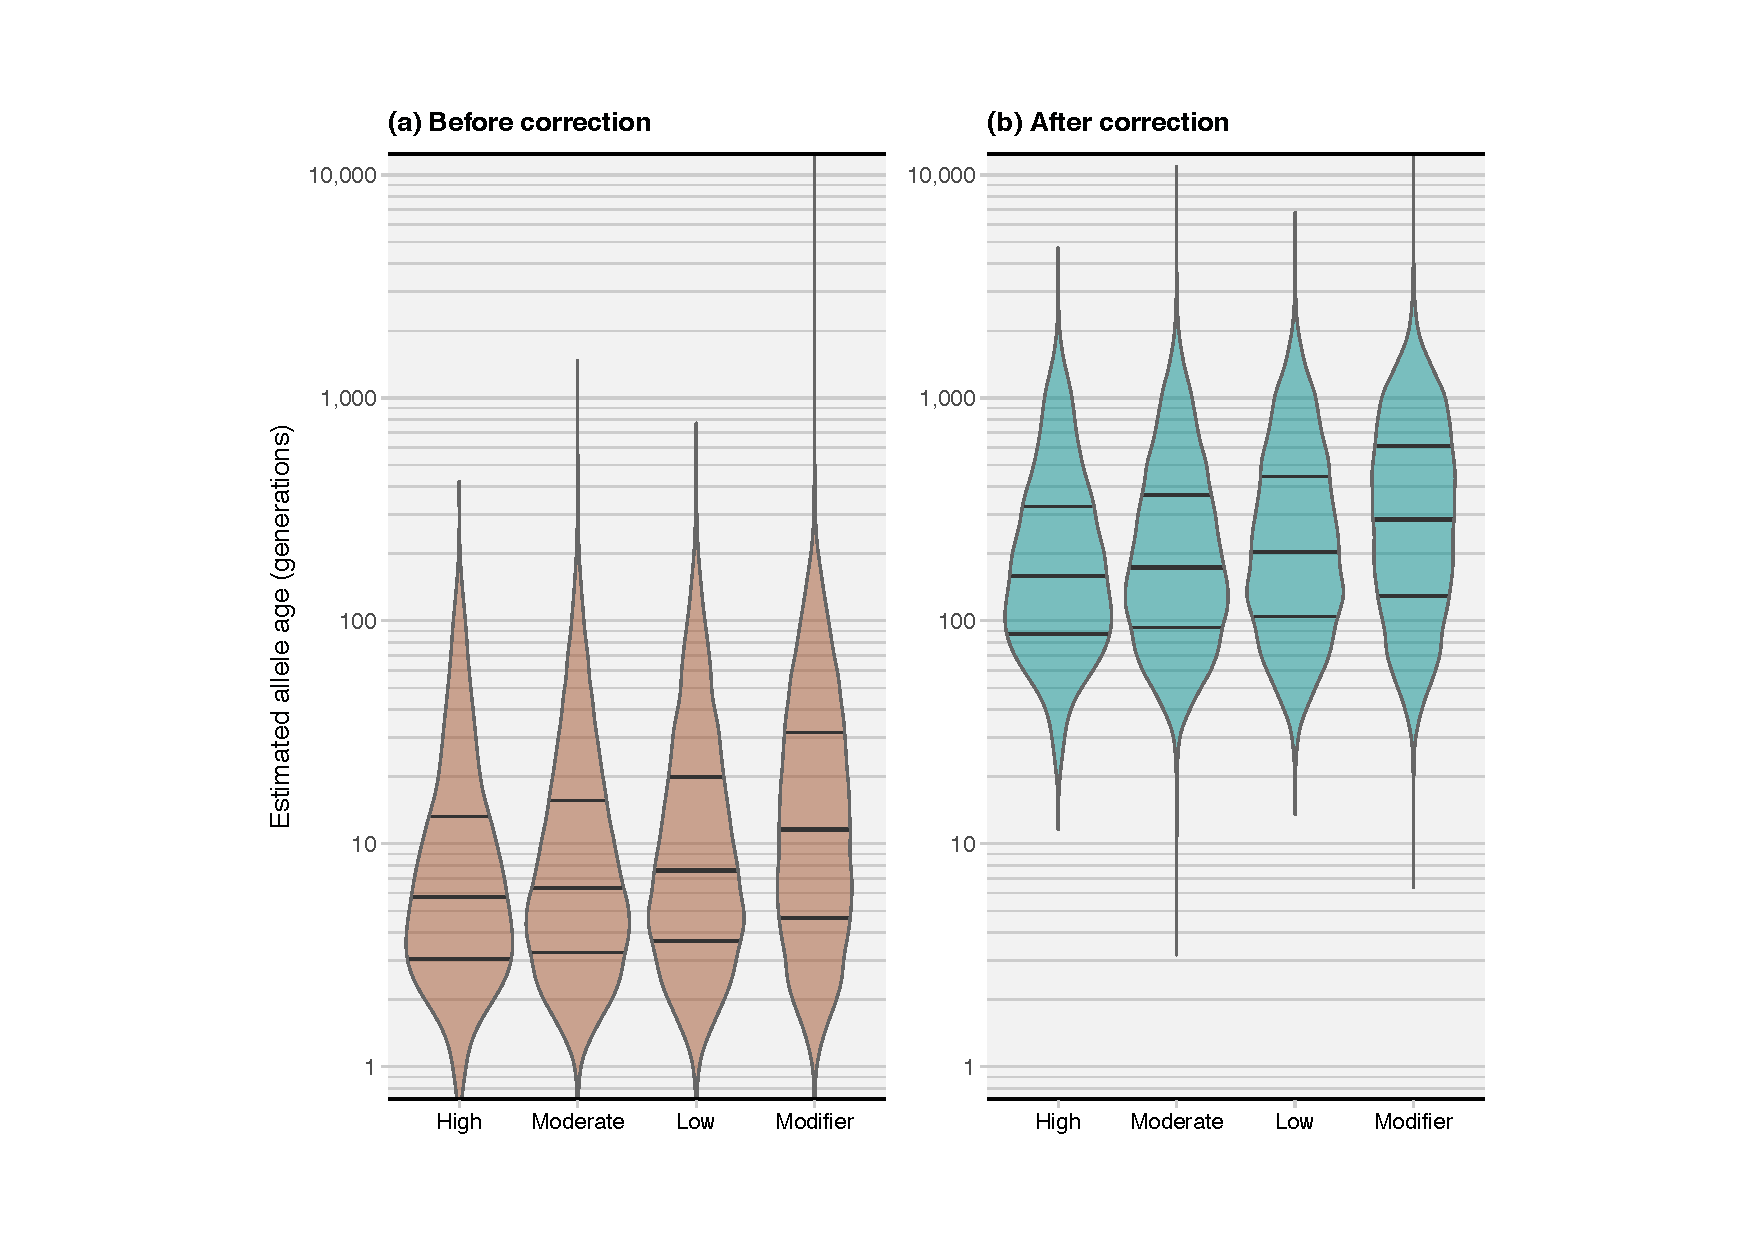
\includegraphics[width=0.75\textwidth]{./img/ch5/1kg_age_impact}
\Caption{Allele age estimated on functionally annotated data in 1000 Genomes}%
{The distribution of inferred allele age is shown in Violin plots by predicted impact category for the whole sample of the \gls{1kg} dataset, before and after correction; \nth{1}, \nth{2}, and \nth{3} quartiles are indicated.}%
{fig:1kg_age_impact}
\end{figure}

% %
%
% The number of retained estimates was \n{141069}, which included
% \n{1255}~variants of \emph{high} impact (splice acceptor and splice donor variants, and stop gained and stop lost variants),
% \n{44131}~variants with \emph{moderate} impact (missense variants only),
% \n{9990}~variants with \emph{low} impact (synonymous variants only), and
% \n{85694}~\emph{modifier} variants (non-coding variants, \eg intron and intergenic variants, and regulatory region variants).
%
% The distribution of allele age before and after correction is shown in \cpref{fig:1kg_age_impact}.
% Before correction, median ages per category were inferred at \numlist{5.6606;6.3292;7.5674;11.8284} generations in \emph{high}, \emph{moderate}, \emph{low}, and \emph{modifier}, respectively, which were corrected to
% \numlist{158.1629;174.4351;203.9523;289.5565} generations, respectively.
% The correlation between estimated age and allele frequency was measured using $r_S$, which was \numlist{0.829272;0.834355;0.850943;0.867078} in \emph{high}, \emph{moderate}, \emph{low}, and \emph{modifier}, respectively.
% Although differences were small, this suggested that the estimated allele age was less correlated with allele frequency if the severity of the presumed consequences was high.
%
% %
% %!TEX root = ../../main.tex


\begin{figure}[p]
{\footnotesize\texthv{\textbf{(a) All alleles analysed}}} \\
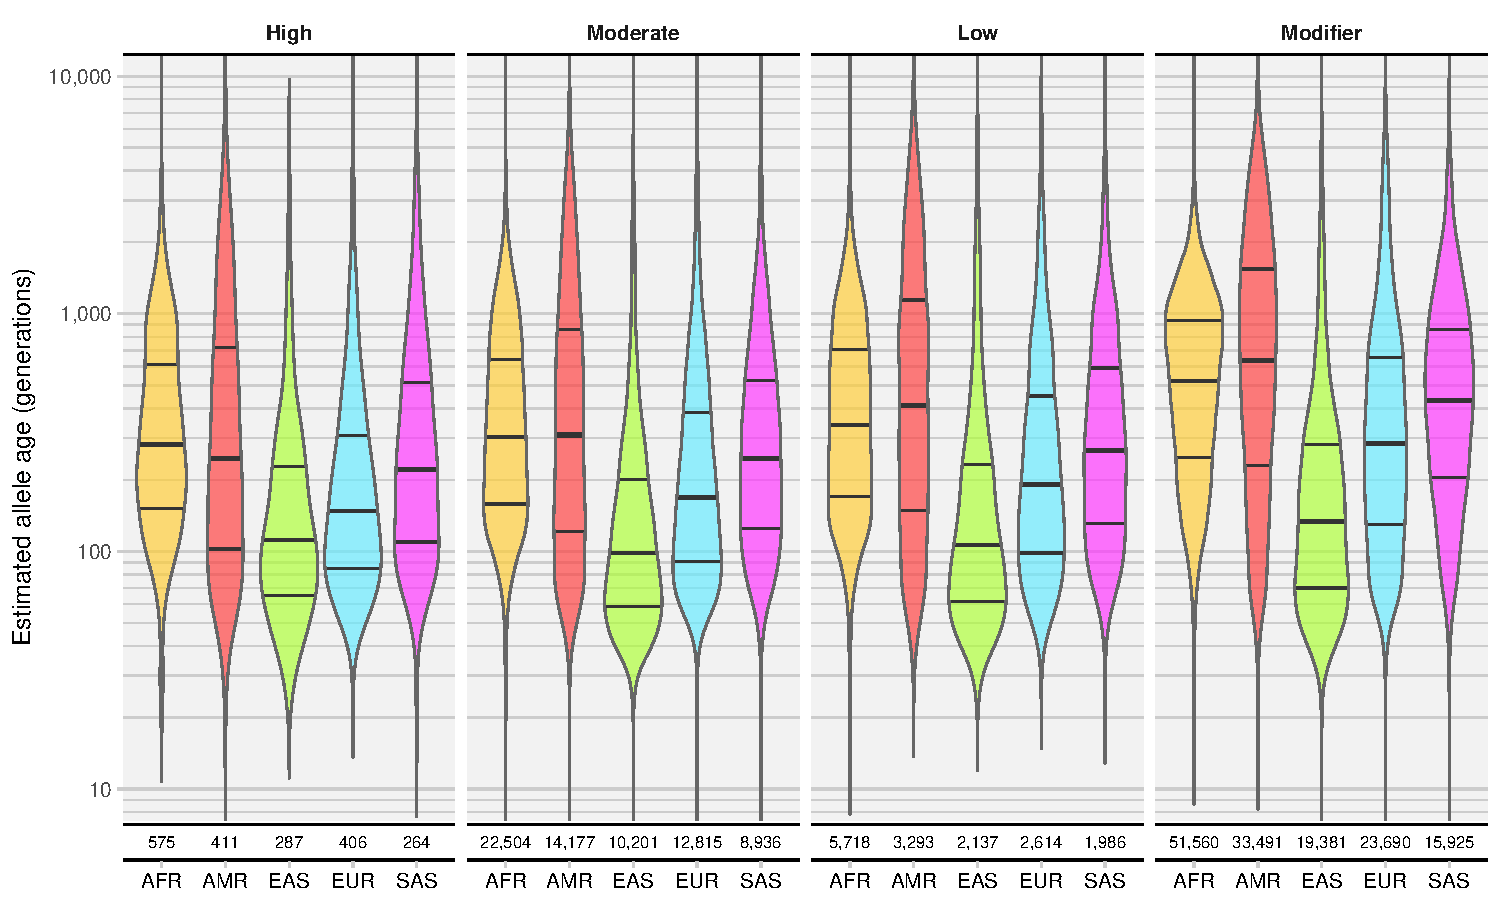
\includegraphics[width=\textwidth]{./img/ch5/1kg_pop_impact_a}
{\footnotesize\texthv{\textbf{(b) Population-specific alleles}}} \\
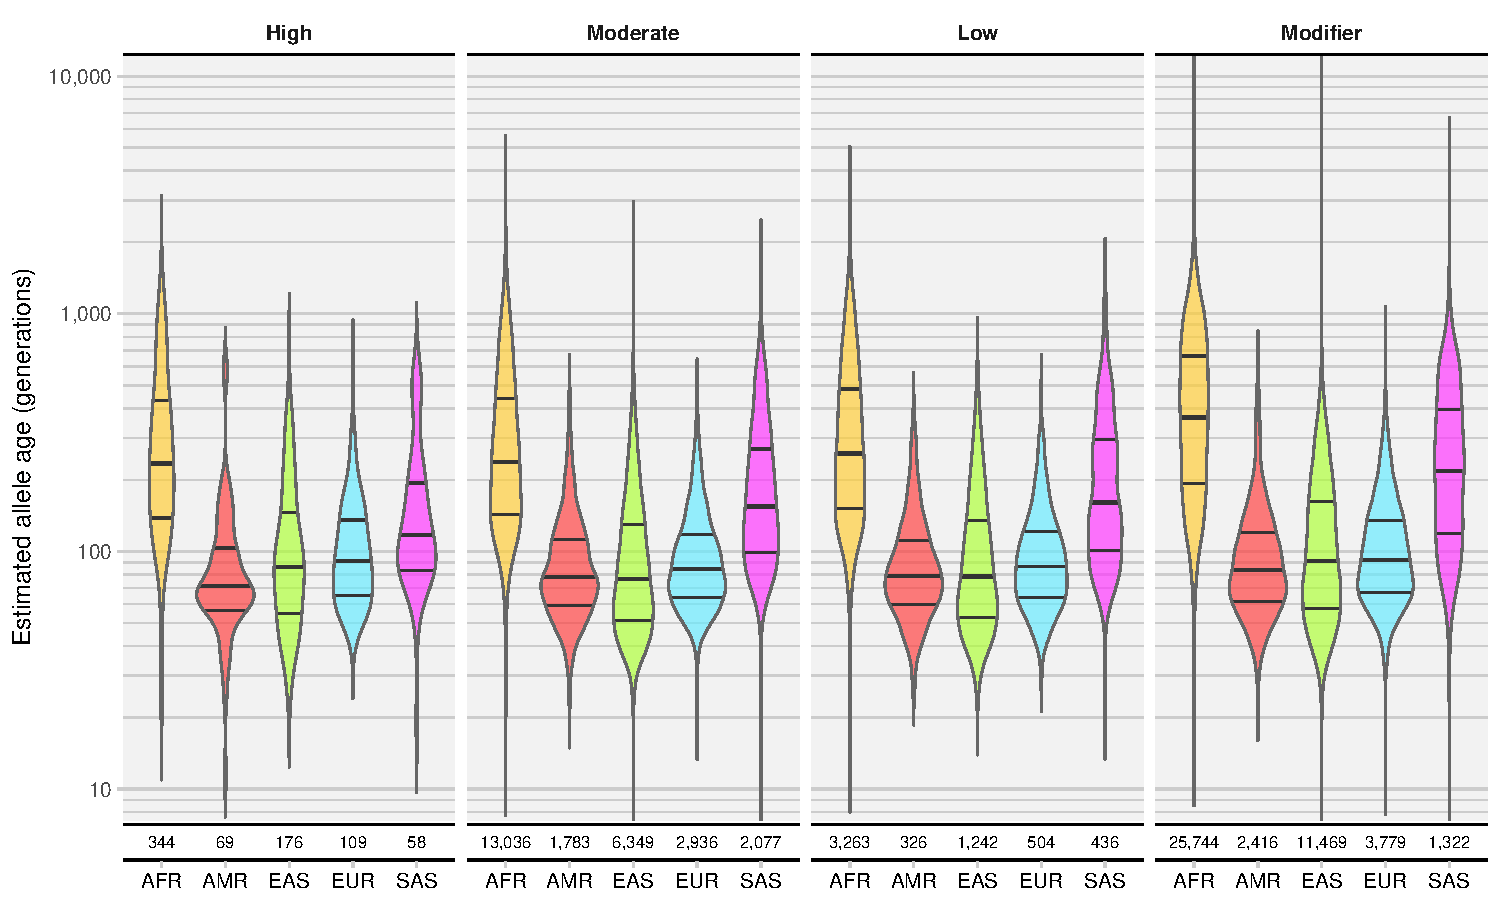
\includegraphics[width=\textwidth]{./img/ch5/1kg_pop_impact_b}
\Caption{Allele age after correction on population-specific frequency in 1000 Genomes}%
{The distribution of inferred allele age is shown in Violin plots by predicted impact category for each population in the \gls{1kg} dataset; \nth{1}, \nth{2}, and \nth{3} quartiles are indicated.
In Panel~\textbf{(a)}, all variants retained after quality control were included in the comparison, which included ${n = \num{141069}}$ target sites.
Note that this also included alleles shared among populations.
In Panel~\textbf{(b)}, only the subset of population-specific variants was included (${n = \num{77438}}$).
The number of alleles retained in each impact category and population are shown below each graph.
The colours used follow the \gls{1kg} colour-scheme.}%
{fig:1kg_pop_impact}
\end{figure}

% %
%
% The \gls{1kg} dataset is composed of several continental population samples (or \emph{super-populations}) in which allele frequencies may differ.
% I applied the correction as per frequency observed in each population; variants were excluded if monomorphic per population.
% Although target sites were selected at ${\leq 1\%}$ allele frequency in the whole sample, some alleles were found at relatively high frequencies in certain populations, but which did not exceed ${5\%}$ allele frequency.
% The distribution of allele age per population is shown in \cref{fig:1kg_pop_impact}{a}.
% Variants of \emph{high} impact were overall estimated to be younger, \eg median age was \dec{276.7156} generations in AFR and \dec{113.8948} generations in EAS.
% Non-coding variants, \emph{modifiers}, were older throughout, \eg \dec{528.8116} generations in AFR, but were not notably older in EAS, where median age was \dec{135.3479} generations.
% Alleles in the AMR sample were overall more widely distributed and indicated an older median age per impact category.
% Rank correlation with allele frequency, $r_S$, was high in AFR (\dec{0.73132}), but not substantial in EAS (\dec{0.43870}), EUR (\dec{0.40936}), and SAS (\dec{0.34668}).
% In AMR, age and frequency appeared to be weakly related (\dec{0.09236}), which may be the result of population admixture, which characterises this population sample.
%
% %
% % !TEX root = ../../main.tex


\begin{table}[!htb]
\Caption{Allele age per population in the 1000 Genomes sample}
{Inferred allele age was corrected in reference to population allele frequencies in the \n{5} population groups in \gls{1kg} data, shown per \gls{vep} impact category.
In total, \n{141070} variants were analysed \textbf{(a)}, of which \n{77439} were population-specific \textbf{(b)}.}
{tab:stats_1kg_impact}
\centering
\begin{tabular}{l*5{S[round-precision=1,table-format=3.1]}*5{S[table-format=1.3]}}
	\toprule
	 Impact & \multicolumn{5}{c}{Median estimated age (generations)} & \multicolumn{5}{c}{Correlation with frequency ($r_S$)} \\
	\cmidrule(lr){2-6}
	\cmidrule(lr){7-11}
	 & {AFR} & {AMR} & {EAS} & {EUR} & {SAS} & {AFR} & {AMR} & {EAS} & {EUR} & {SAS} \\
	\otoprule
	\multicolumn{11}{@{\,}l}{(a) All alleles analysed} \\
	\midrule
	\textit{High    } &  276.7156 & 238.2880 & 113.8948 & 145.7969 & 219.0302  &  0.697134 & 0.164036 & 0.444797 & 0.581463 & 0.441301 \\
	\textit{Moderate} &  305.1702 & 311.4755 &  99.0084 & 169.0662 & 247.7381  &  0.707347 & 0.143252 & 0.432302 & 0.469482 & 0.385978 \\
	\textit{Low     } &  341.4061 & 413.9554 & 105.0124 & 191.9495 & 266.3468  &  0.737771 & 0.116200 & 0.388013 & 0.445391 & 0.410477 \\
	\textit{Modifier} &  528.8116 & 645.6322 & 135.3479 & 287.2691 & 435.3400  &  0.728619 & 0.058309 & 0.435299 & 0.349477 & 0.339951 \\
	\otoprule
	\multicolumn{11}{@{\,}l}{(b) Population-specific alleles} \\
	\midrule
	\textit{High    } &  227.2396 & 67.6673 & 86.8637 & 87.8490 & 116.6994  &  0.885856 & 0.672827 & 0.860747 & 0.738088 & 0.864570 \\
	\textit{Moderate} &  239.8254 & 77.3700 & 76.8140 & 84.6032 & 154.8731  &  0.891540 & 0.647132 & 0.877686 & 0.745509 & 0.906612 \\
	\textit{Low     } &  256.4403 & 78.0054 & 77.9945 & 87.1812 & 154.9337  &  0.904668 & 0.616386 & 0.880905 & 0.751465 & 0.907093 \\
	\textit{Modifier} &  369.7328 & 82.7324 & 91.8433 & 91.8594 & 221.5612  &  0.919745 & 0.706728 & 0.896563 & 0.807821 & 0.934936 \\
	\bottomrule
\end{tabular}
\end{table}

% %
%
% Variants that appeared in more than \n{1} population were removed to focus on population-specific, presumably more recent alleles; see \cref{fig:1kg_pop_impact}{b}.
% This reduced the number of alleles to \n{77438}.
% Notably, alleles retained in AMR were youngest in all impact categories, whereas the alleles specific to the AFR sample were seen to be the oldest; \eg median age was \dec{227.2396} generations in \emph{high} and \dec{369.7328} generations in the \emph{modifier} category.
% Rank correlation between between allele frequency and inferred age showed a more consistent relationship in each population;
% AFR (\dec{0.91654}), EAS (\dec{0.89046}), EUR (\dec{0.77979}), SAS (\dec{0.92096}).
% Notably, the variants specific to AMR now showed a moderately high correlation between age and frequency (\dec{0.67690}).
% These results are summariesed in \cpref{tab:stats_1kg_impact}.
%





% First, correct age estimation may be affected due to its reliance on correct IBD inference, where inaccurate detection of IBD segments was shown to affect the estimation differently under each of the \n{3} clock models.
% Second, even if IBD is detected with high accuracy, the alleles observed at a focal variant in the sample may wrongly identify individuals through
% haplotype sharing may not be
% a focal allele may incorrectly identify haplotype sharing in the sample.
% In particular, the \n{2} types of error are \emph{false positives} (Type~1 error), where an allele wrongly identifies haplotype sharing, and \emph{false negatives} (Type~2 error), where an allele was missed.
% Both types affect

% misclassified alleles along the shared sequence may artificially inflate the genetic length number of pairwise differences, $S$, seen between haplotype sequences, which affects both the mutation clock, \ClockM, and the combined clock, \ClockC.
% I showed that the impact of phasing error is small compared to genotype error, which is relevant when the \gls{fgt} is used for IBD detection.
% When the \gls{dgt} or the \gls{hmm}-based approach is used, the misclassification of genotypes is the main source of error.
% Third, the analysis is likely to be biased if the alleles observed at a target site incorrectly identify haplotype sharing in the sample.



% \begin{description}
% 	\item[\textbf{Type \rom{1}}] errors or \emph{false positives}
% 	\item[\textbf{Type \rom{2}}] errors or \emph{false negatives}
% \end{description}



%
%
% New results below
%
%


\AdditionNote{All sections below were added to include new results as presented in the viva}


%
\section{A haplotype-based HMM for shared haplotype inference}
%

As shown in the previous sections, the allele age estimation method was able to infer the time of mutation events with high accuracy, but where it was suggested that this is largely dependent on (ideally) correct inference of the underlying shared haplotype structure around a given target site.
The inference methods presented so far were either rule-based (\gls{fgt} and \gls{dgt}) and thus highly susceptible to data error, or probabilistic but genotype-based (\gls{hmm}) where accuracy may easily be influenced by the shared haplotype structure at the ``unshared'' haplotypes in the individuals considered.
Although the latter was implicitly impervious to data error due to phasing, it was shown that such errors were less problematic on average, but where error due to misclassification of alleles may be regarded as the main source of estimation bias.

In this section, I present a novel haplotype-based \gls{hmm} for the targeted and pairwise detection of shared haplotypes.
This method can be seen as the conclusion of the previous genotype-based approach and is therefore algorithmically defined in a similar way.
I describe the model in the section below.
Note that I implemented additional modifications in the age estimation method, which I describe in \cpref{sec:age_method_mod}.

As done previously, I evaluated the haplotype-based \gls{hmm} in terms of the resulting age estimation accuracy in data before and after error (\ccref{sec:hhmm_eval}).
The method was further compared to the \gls{psmc} in terms of the inferred \gls{tmrca} and subsequent estimation of allele age (\ccref{sec:psmc_eval}).
Lastly, I briefly present age estimation results from an analysis using \glsentryfull{1kg} Phase~\rom{3} data (\ccref{sec:hhmm_1kg}).


%
\subsection{Description of the model}
%

The general algorithm and model specifications of the \gls{hmm} presented here follow the previously described genotype-based \gls{hmm}; see \cpref{sec:ghmm_algorithm}.
Briefly, at a given target position in the genome, the allelic sequence of \n{2} selected haplotypes is independently traversed to the left and right-hand side from that position, until the end of the chromosome is reached.
As before, \n{2} hidden states are assumed; \emph{ibd} and \emph{non}.
The observation states are defined as the possible allelic pairs $(0,0)$, $(0,1)$, and $(1,1)$, where the order of alleles is not relevant; \ie observing $(0,1)$ in haplotypes $A$ and $B$ is equivalent to observing $(1,0)$.
The model is illustrated in \cpref{fig:info_hmm_hap}, where $\varphi$ denotes a transition parameter and the probabilities of emission from \emph{ibd} are denoted by $\delta_{h_A h_B}$ and from \emph{non} by $\eta_{h_A h_B}$.
Model transitions, emissions, and initial state probabilities are described below.


%
%!TEX root = ../../main.tex


\begin{figure}[!htb]
\centering
%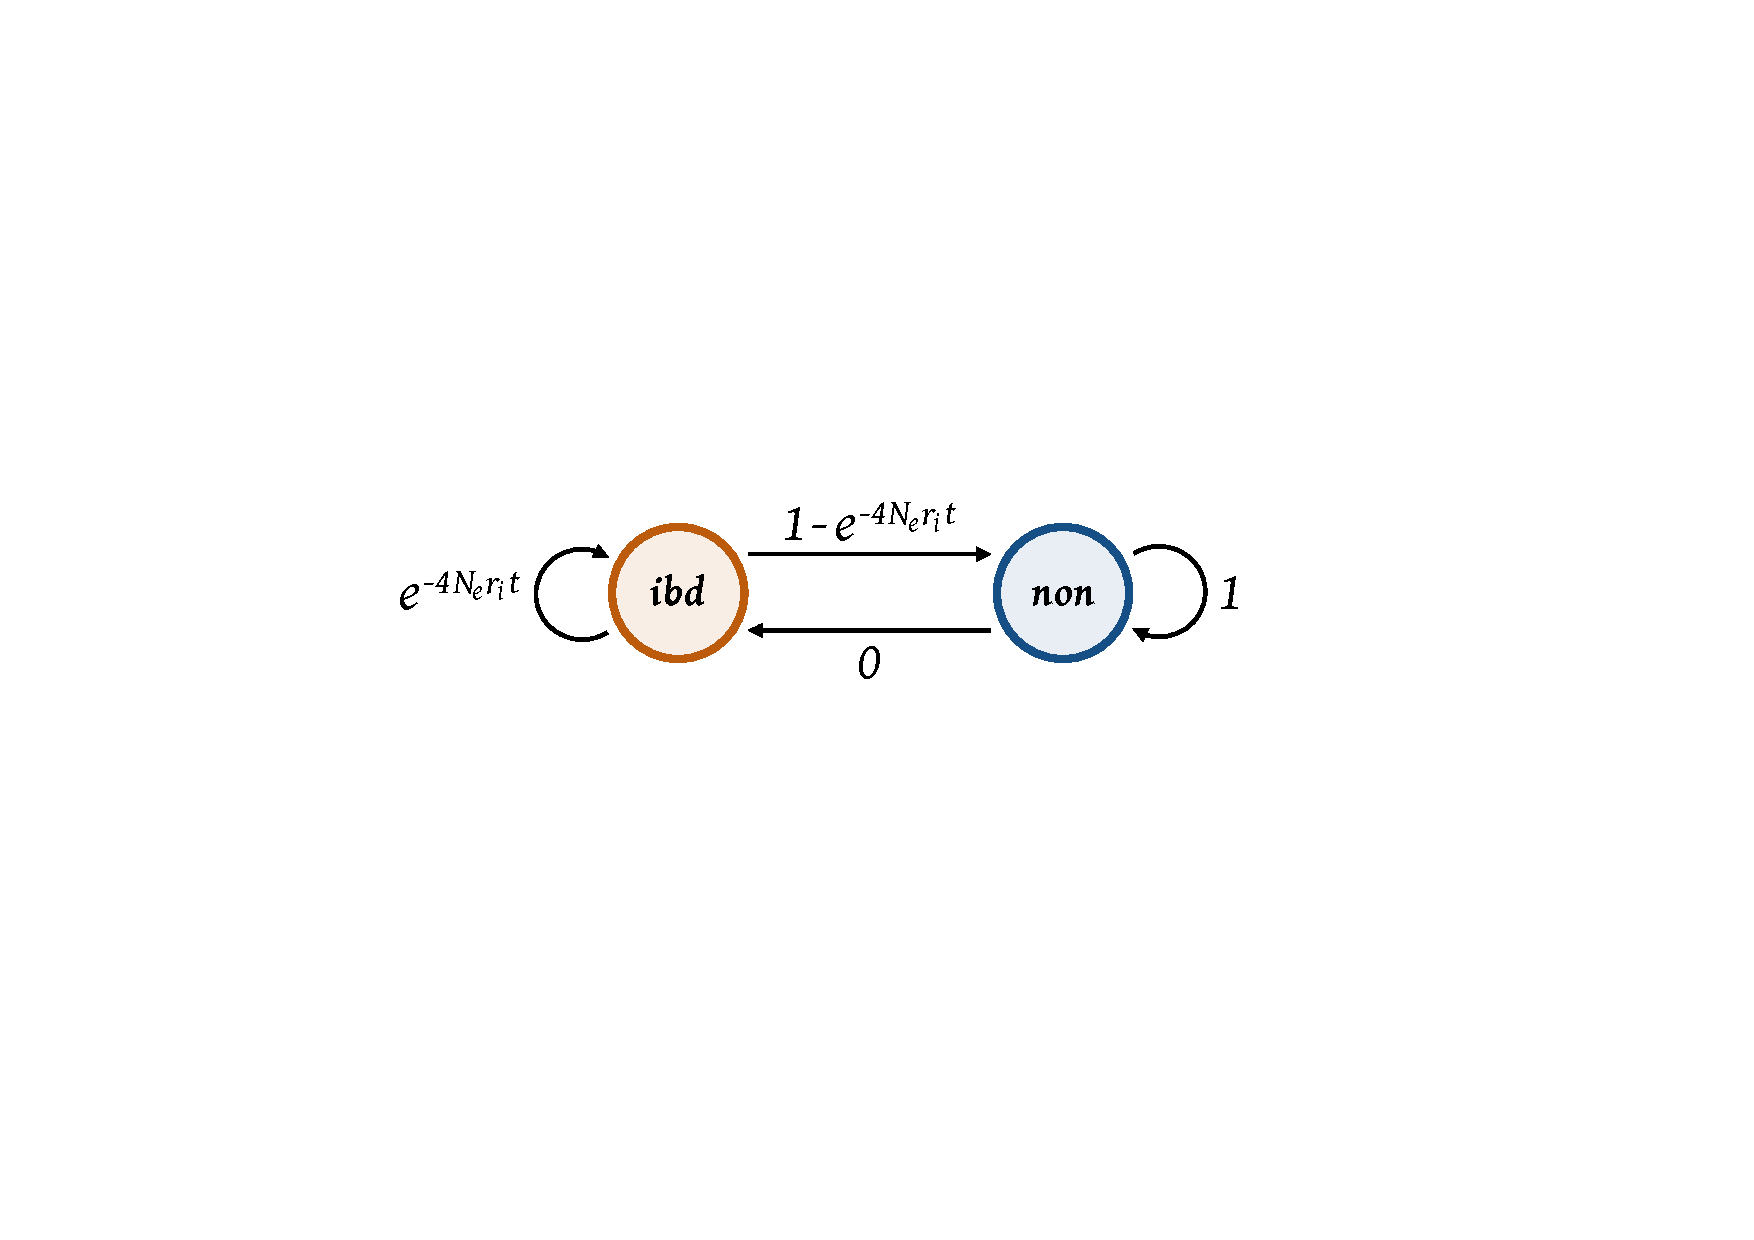
\includegraphics[width=0.75\textwidth]{./img/ch4/hmm_trans}\\

\vspace{5pt}
\begin{tikzpicture}[->,>=stealth,auto,thick,
txt/.style={font=\sffamily\small,text width=2.5cm},
sub/.style={circle,draw=white, fill=white,minimum size=1.75cm},
state/.style={circle,draw,ultra thick,minimum size=1.5cm,outer sep=2pt,font=\bfseries\Large},
dbl/.style={diamond,draw=black!50,thick,minimum size=1.45cm,outer sep=2pt},
obs/.style={diamond,draw=black,fill=white,fill opacity=0.5,text opacity=1,thick,minimum size=1.5cm,outer sep=2pt,font=\bfseries}]

\newcommand{\observeIBD}[4]{
\draw[->,draw=DarkOrange2!20,ultra thick] (#1) to (#2);
\draw[->,draw=DarkOrange3,densely dotted] (#1) -- (#2) node [pos=#4,anchor=center,fill=white,font=\small,inner sep=2pt] {#3};
}
\newcommand{\observeNON}[4]{
\draw[->,draw=DodgerBlue3!20,ultra thick] (#1) to (#2);
\draw[->,draw=DodgerBlue4,densely dotted] (#1) -- (#2) node [pos=#4,anchor=center,fill=white,font=\small,inner sep=2pt] {#3};
}

\node[txt] at (0, 4) {Hidden\\states};
\node[txt] at (0, 0) {Observation\\states};

\node[sub] (I) at (3.5,4) {};
\node[sub] (N) at (8.5,4) {};

\node[state,draw=DarkOrange3,fill=DarkOrange1!25] (ibd) at (3.5,4) {\emph{ibd}};
\node[state,draw=DodgerBlue4,fill=DodgerBlue1!25] (non) at (8.5,4) {\emph{non}};

% \node[dbl] (s00) at (1,0.84) {};
% \node[dbl] (s01) at (3,0.84) {};
% \node[dbl] (s02) at (5,0.84) {};
% \node[dbl] (s11) at (7,0.84) {};
% \node[dbl] (s12) at (9,0.84) {};
% \node[dbl] (s22) at (11,0.84) {};

\node[obs] (h00) at (2,0)  {$h_{00}$};
\node[obs] (h01) at (6,0)  {$h_{01}$};
\node[obs] (h11) at (10,0) {$h_{11}$};

% \path (ibd.25)  edge node[above]{\Large{${1 - e^{-4 \Ne r_i \tau_k}}$}} (non.155);
\path (ibd.25)  edge node[above]{\large{$\varphi$}} (non.155);
\path (non.205) edge node[below]{\large{$0$}} (ibd.335);

% \path (ibd) edge [out=205,in=155,looseness=5] node[left] {\Large{${e^{-4 \Ne r_i \tau_k}}$}} (ibd);
\path (ibd) edge [out=205,in=155,looseness=5] node[left] {\large{$1-\varphi$}} (ibd);
\path (non) edge [out=25,in=335,looseness=5] node[right] {\large{$1$}} (non);

% \observeIBD{I.315}{g22}{$\delta_{22}$}{0.25}
% \observeIBD{I.300}{g12}{$\delta_{12}$}{0.31}
% \observeIBD{I.285}{g11}{$\delta_{11}$}{0.4}
\observeIBD{I.300}{h11}{$\delta_{11}$}{0.2}
\observeIBD{I.280}{h01}{$\delta_{01}$}{0.35}
\observeIBD{I.260}{h00}{$\delta_{00}$}{0.5}

\observeNON{N.240}{h00}{$\eta_{00}$}{0.2}
\observeNON{N.260}{h01}{$\eta_{01}$}{0.35}
\observeNON{N.280}{h11}{$\eta_{11}$}{0.5}
% \observeNON{N.270}{g11}{$\eta_{11}$}{0.5}
% \observeNON{N.285}{g12}{$\eta_{12}$}{0.45}
% \observeNON{N.300}{g22}{$\eta_{22}$}{0.45}

\end{tikzpicture}
% \vspace{10pt}
%
% X
%
% \vspace{10pt}
% \begin{tikzpicture}[auto,thick,decoration={coil},
% line/.style={->,>=latex},
% rec/.style={->,>=stealth,rounded corners=4pt},
% txt/.style={font=\sffamily\small,text width=2.5cm},
% dna/.style={decorate,thick,decoration={aspect=0, segment length=0.5cm}},
% var/.style={rectangle,draw=black!50,fill=black!10,minimum size=0.4cm,outer sep=2mm,inner sep=2pt,font=\tiny\sffamily\bfseries}]
%
% \node[txt] at (-1, 5) {Genome};
% \node[txt] at (-1, 3.5) {Sample variant sequence};
%
% % \node[var] at (2.1,0) {};
% % \node[var] at (3.5,0) {};
%
% \foreach \v [remember=\v as \last (initially 1), count=\i] in {1.94,2.87,4.05,4.71,5.86,7.37,8.63,9.66,10.38}{
% 	\fill[gray!50] (\v - 0.05,4.6) rectangle (\v + 0.05,5.4);
% 	\coordinate (beg) at (\v,4.4);
% 	\node[var]  (end) at (\v,3.4) {\i};
% 	\draw[line] (beg) to (end.north);
% }
%
% \draw[dna, decoration={amplitude=.15cm}] (1.1,5) -- (11.5,5);
% \draw[dna, decoration={amplitude=-.15cm}] (1,5) -- (11.5,5);
%
% \fill[white] (0.9,4.6) rectangle (1.13,5.4);
% \fill[white] (11.2,4.6) rectangle (11.6,5.4);
%
% % \node[site] (1) at (1.0,2) {};
% %
% % \foreach \s [remember=\s as \last (initially 1)] in {2,...,10}{
% %   \node[site] (site\s) at (\s,2) {};
% %   \draw[line] (\last,2) to (site\s.west);
% % 	\node[site] (\s) at (\s,2) {};
% % }
%
% \end{tikzpicture}

\vspace{5pt}

\Caption{Illustration of the haplotype-based HMM for shared haplotype inference}%
{\N{2} hidden states are assumed to generate the observations in a Markov process; \emph{ibd} and \emph{non}.
Transitions from each state into any state are indicated by \emph{solid} lines.
The probability of transition from \emph{ibd} to \emph{non} is denoted by $\varphi$, and from \emph{non} to \emph{ibd} is set to zero; hence, once the chain proceeds into the \emph{non} state it cannot go back into \emph{ibd}.
This is because the process is modelled such that only the innermost segment is inferred, relative to the focal position which sits at the start of the sequence.
The input sequence consists of sequence data from a pair of haplotypes, resulting in \n{3} possible observation states; denoted by $h_{h_A h_B}$, where ${h_A,h_B \in \lbrace 0,1 \rbrace}$.
The probabilities of emitting each possible haplotype pair given each hidden state are denoted by $\delta_{h_A h_B}$ and $\delta_{h_A h_B}$ for \emph{ibd} and \emph{non}, respectively; indicated by the \emph{dotted} lines.
The direction of arrows indicates conditional dependence; \ie the transition from one hidden state into another state, or emission of a genotype pair while being in \emph{ibd} or \emph{non}.}%
{fig:info_hmm_hap}
\end{figure}

%

\paragraph{Transition probabilities.}
The genetic distance to a recombination event follows the Exponential distribution when measured in population-scaled time units.
The probability of transition from \emph{ibd} to \emph{non} is modelled as
\begin{equation}\label{eq:hmm_trans_prob}
	\varphi ~=~
	1 - \euler{-2\Ne r_j \frac{\xi_k}{2}}
\end{equation}
where $j$ indicates the position at the current site in the sequence and $k$ indicates the the focal position.
The value of $r_j$ is the genetic distance between the current and the Immediately previous site observed in the sequence.
The value of $\xi_k$ is the expectation of the age of the focal allele after \citet{Kimura:1973ug}, calculated using \ctref{eq:intro_kimura_ohta}.
The probability of remaining in \emph{ibd} is ${1-\varphi}$.
The model employs a ``left-to-right'' architecture, where transition from \emph{non} to \emph{ibd} have zero probability; \ie once \emph{ibd} has been left the sequence stays in \emph{non} with probability equal to one.
The intuition and shortcomings of such a transition model were discussed in \cpref{sec:HmmTrans}.



\paragraph{Emission probabilities.}
An empirical emission model was generated from simulated haplotype data, both before and after the integration of empirically determined error rates.
In the previous genotype-based model, the empirical rate of observing possible genotype pairs was determined from haplotype segments shared between individuals who carried any allele observed at low frequency (\fk{[2,25]}).
The same was done here, but such that the empirical probabilities were measured based on the \gls{tmrca} between haplotype pairs.
A full representation of observation rates found by \gls{tmrca} and allele frequency is given in \cpref{fig:hhmm_emission_tmrca}.
Note that, again, datasets $\mathcal{D}_B$ and $\mathcal{D}_B^{\ast}$ were used to obtain emission models before and after error.

%
% !TEX root = ../../main.tex


\begin{figure}[!htb]
\centering
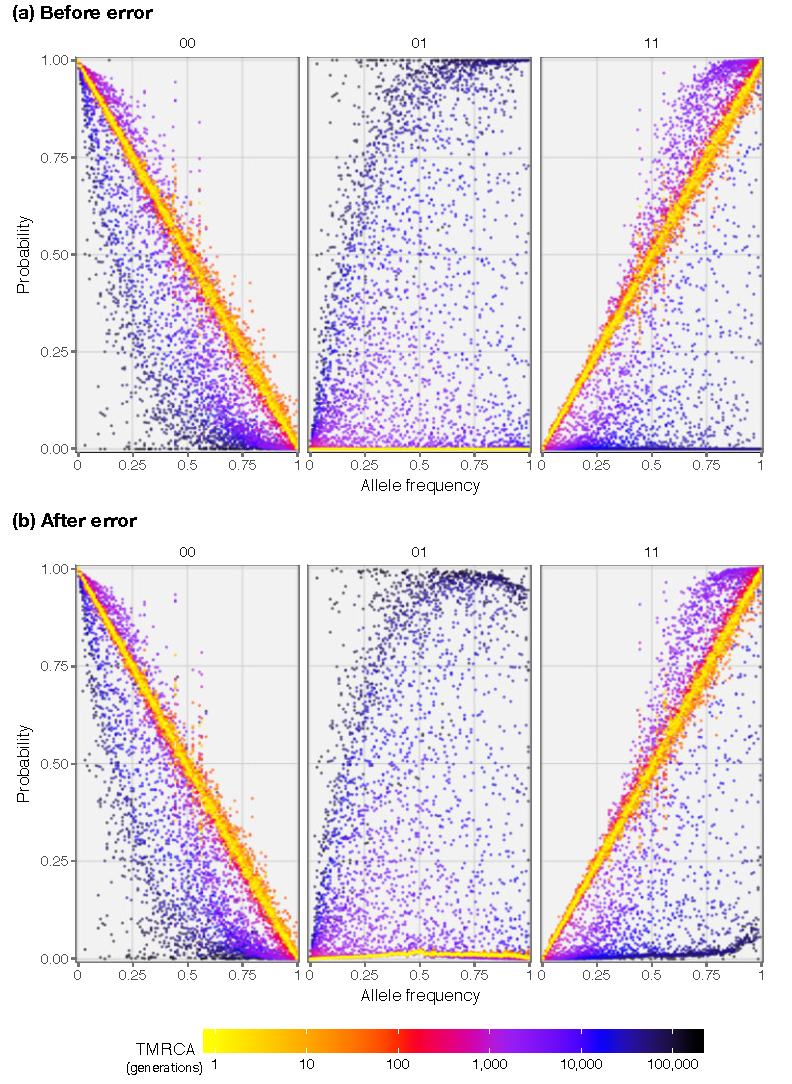
\includegraphics[width=0.75\textwidth]{./img/ch5/hhmm_emission_tmrca_lowres}
\Caption{Empirical probability to observe allelic pairs dependent on T\textsubscript{MRCA}}
{Using data before and after error (datasets $\mathcal{D}_B$ and $\mathcal{D}_B^{\ast}$), the rate at which the possible allelic pairs $(0,0)$, $(0,1)$, and $(1,1)$ were observed is shown by allele frequency, distinguished by the \gls{tmrca} between two haplotypes at a given site.
Empirical observation rates were measured at \n{100000} randomly selected haplotype pairs.
The resulting rates were averaged over \n{100} equally sized allele frequency bins and \n{100} time intervals of equal size on log-scale.
Panels \textbf{(a)} and \textbf{(b)} show the empirical distribution before and after error, respectively.}
{fig:hhmm_emission_tmrca}
\end{figure}

%

However, the generation of the emission model was not straightforward as any pair of haplotypes is
“identical by descent” at any position in the genome; according to the coalescent and the assumptions of the infinite sites model.
The definition of the hidden states as being ``in IBD'' and ``not in IBD'' may therefore be seen as arbitrary.
Nonetheless, to generate empirical probabilities,
I defined a nominal ``cutoff'' for the \gls{tmrca} at \n{100} generations to calculate the mean empirical observation rates for each state.
The average rate seen ${\leq 100}$ generations was taken for \emph{ibd}, and
$>100$ generations for \emph{non}, at each allele frequency bin (rates were averaged over \n{100} equally sized bins).
Linear interpolation was used to obtain rates at sites with frequencies not captured by the model.
The resulting model is illustrated in \cpref{fig:hhmm_emission_model}.

%
% !TEX root = ../../main.tex


\begin{figure}[!htb]
\centering
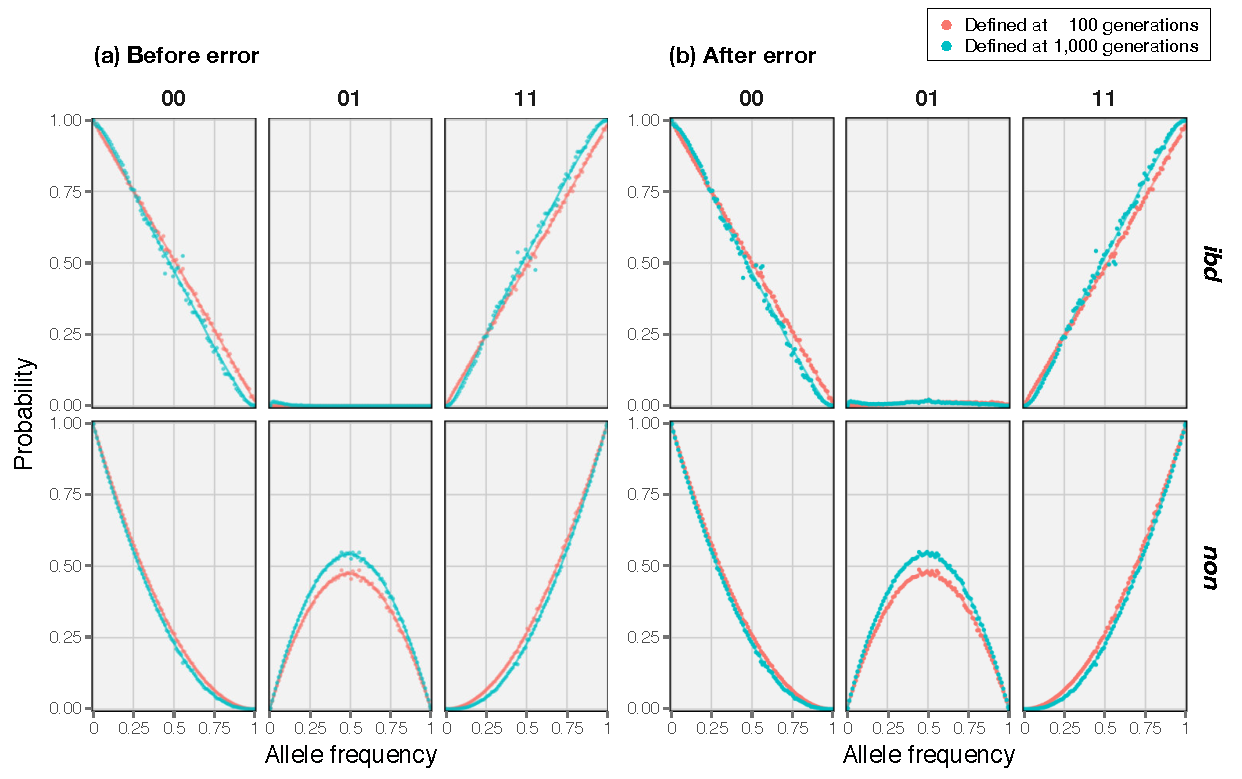
\includegraphics[width=\textwidth]{./img/ch5/hhmm_emission_model_lowres}
\Caption{Empirical emission model used in the haplotype-based HMM}
{The emission probabilities used in the haplotype-based HMM were determined empirically for each possible allelic pair, using datasets $\mathcal{D}_B$ (before error) and $\mathcal{D}_B^{\ast}$ (after error).
To distinguish \emph{ibd} from \emph{non}, a nominal cutoff was applied to the result shown in \cpref{fig:hhmm_emission_tmrca}.
For comparison, the resulting distributions for a \gls{tmrca} cutoff at \n{100} generations (\emph{red}) are compared to a cutoff at \n{1000} generations (\emph{blue}).}
{fig:hhmm_emission_model}
\end{figure}

%

One caveat of applying such a cutoff is that the model is implicitly conditioned on observations deriving from relatively recent coalescent events.
But, notably, when comparing cutoffs at \n{100} and \n{1000} generations, differences between averaged distributions were relatively small; as shown in \cref{fig:hhmm_emission_model}.
In the following, the emission models generated from dataset $\mathcal{D}_B$ were used in all analyses of error-free data; otherwise, the model generated from $\mathcal{D}_B^{\ast}$ was used.



\paragraph{Initial state probabilities.}
The estimated true positive rate of observing allelic pairs in data before and after error was taken as an empirical model of the initial state probabilities.
Note that for error-free data implies the initial probability of being in \emph{ibd} is equal to one, as it is certain that a focal haplotype pair shares an allele by descent at a given target site; given the assumptions of the infinite sites model.
Again, datasets $\mathcal{D}_B$ and $\mathcal{D}_B^{\ast}$ were used.

%
% !TEX root = ../../main.tex


\begin{figure}[!htb]
\centering
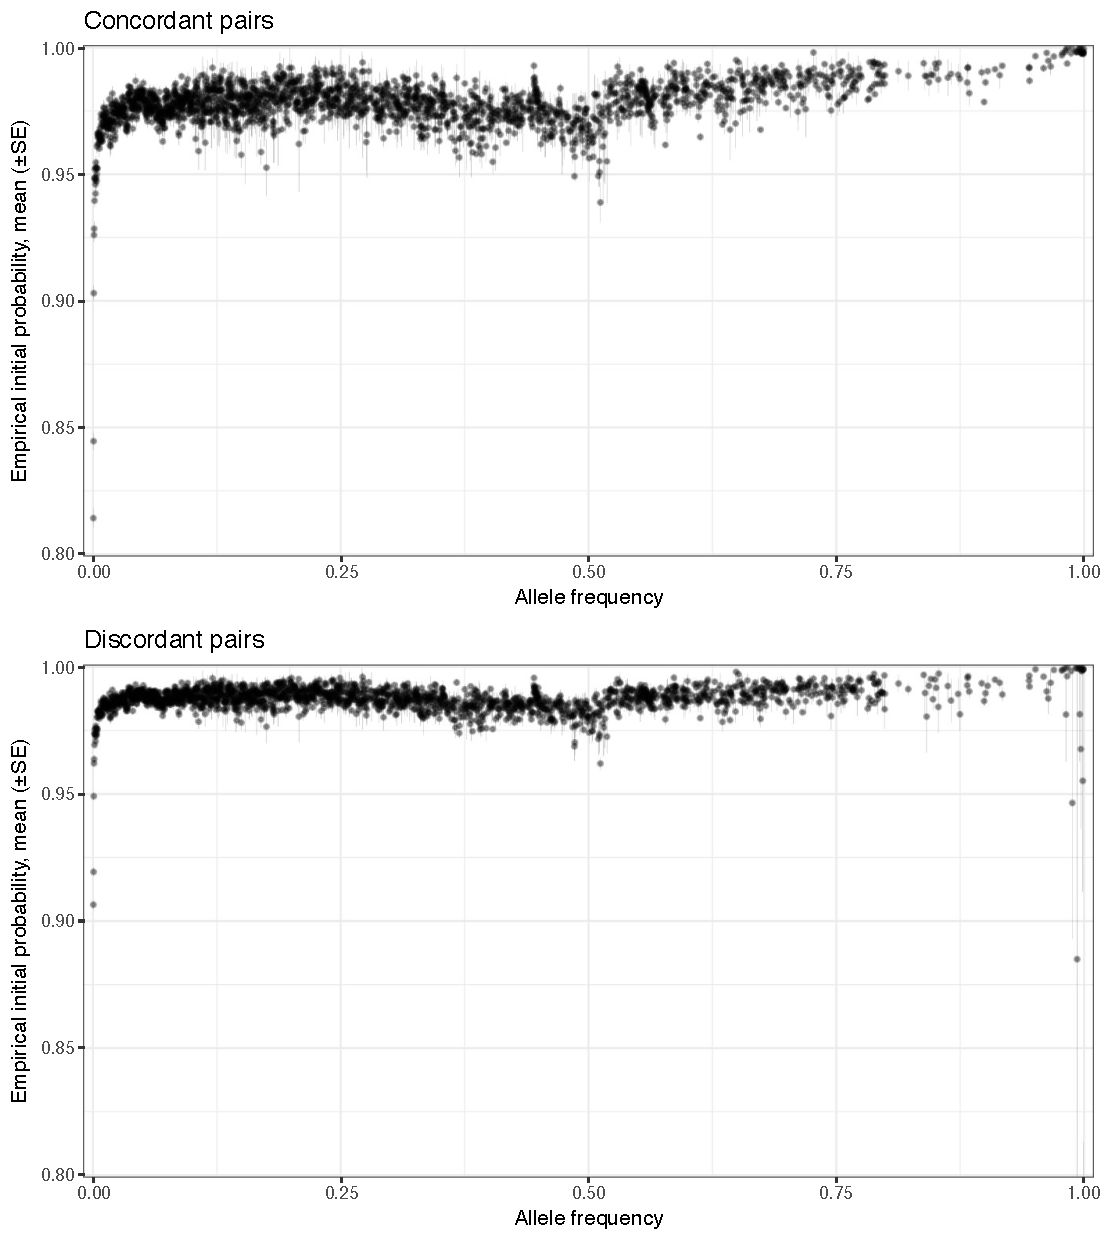
\includegraphics[width=0.75\textwidth]{./img/ch5/hhmm_initial_model_lowres}
\Caption{Empirical initial state probabilities used in the haplotype-based HMM}
{The rate of correctly observing allelic combinations in pairs of haplotypes was measured by comparing data points before and after error, using simulated datasets $\mathcal{D}_B$ and $\mathcal{D}_B^{\ast}$.
At a given focal site, haplotypes were sorted into concordant and discordant pairs as determined from allele sharing in the sample before error.
The allelic state at each pair was then compared to the same location and pair in data after error, to measure the true positive rate of observing the $(1,1)$ allelic combination in concordant pairs and $(0,1)$ in discordant pairs.
Rates are shown as the mean for observations at a given focal allele count ($\pm$SE).
The number of focal sites observed at a specific frequency in the sample differed along the site frequency spectrum, but was capped at a maximum of \n{1000} randomly sampled sites found at a given allele count.}
{fig:hhmm_initial_model}
\end{figure}

%

Empirical rates were estimated as follows.
At a given site, the sample was distinguished into carrier and non-carrier haplotypes for the allele at that site to form all possible concordant and discordant pairs.
Each pair was analysed in turn where allele combinations were compared before and after error to establish the rate at which alleles were observed correctly at that site and that pair.
That is, allelic combinations $(1,1)$ in concordant pairs and $(0,1)$ or $(1,0)$ in discordant pairs.
This was done at each value of the allele count in the simulated dataset ($N=\n{5000}$ haplotypes), but where a maximum of \n{1000} randomly selected sites was analysed from the sites found at the same allele count.
Measured rates were then averaged per bin; the result is shown in \cpref{fig:hhmm_initial_model}.
When applied to data of different size $N$, rates were linearly interpolated based on allele frequency.






%
\subsection{Modifications of the age estimation method}\label{sec:age_method_mod}
%

I attempted to improve the allele age estimation method as a result of the lessons learned from the analyses conducted in previous sections.
Note that the implemented modifications entail (minor) changes to the algorithm, but where model specifications remained untouched.

%
\subsubsection{Nearest neighbour selection of discordant pairs}
%

Discordant pairs are formed by taking one haplotype from set $X_c$ (\emph{carriers}) and one from set $X_d$ (\emph{non-carriers}).
The intuition is that discordant pairs can be used to indicate the time of coalescent events above the point in time at which the focal mutation occurred (back in time), such that the ``upper limit'' of the branch can be found.
It would be beneficial to select those haplotypes from $X_d$ that are the nearest neighbours to the sub-tree spanned by the lineages leading to $X_c$.
Otherwise, if selection of pairs is random, the number of discordant pairs required to include nearer neighbours may be relatively high on average, dependent on the composition of the sample.

I implemented a simple approach to calculate the Hamming distance in each discordant pair in the sample, along a fixed region around the focal site.
Discordant pairs with the lowest distance are prioritised.
Here, the first \n{5000} sites to the left and right-hand side of the focal position were queried.

Importantly, in presence of data error, it is likely that false negatives (missed focal alleles) would be selected preferentially.
To reduce the chance of selecting false negatives, I used a ``relaxed'' nearest neighbour approach.
Discordant pairs are first sorted by their distance (lowest to highest) and each pair is scanned in turn.
I then identify $X_d$ haplotypes that are repeated more than once along the queue of pairs and place these at the end of the queue.
The first $n_d$ pairs are then retained, where $n_d$ can be specified.

The implementation of this algorithm substantially improved computation time due to retaining a smaller number of pairs.
The results presented below were obtained using only $n_d=100$ discordant pairs (as opposed to several hundreds or thousands of randomly selected pairs).
Note that a nearest neighbour approach could also be applied to select concordant pairs (prioritising higher distances), but which was not done here, as it is assumed that random sampling is sufficient to retain pairs that indicate coalescent events close to the time of the focal mutation event.




%
\subsubsection{Restriction of counting pairwise differences in concordant pairs}
%

Misclassification of genotypes or alleles is expected to adversely affect estimation accuracy when the mutation clock or the combined clock model is used.
False negatives (missed alleles) and false positives (wrongly called or typed alleles) if not consistent in both haplotypes may artificially inflate the number of pairwise differences seen along the inferred shared haplotype region.

I implemented a simple rule to restrict the count of pairwise differences.
At a given site along the sequence, an observed difference is only counted if its frequency in the sample is less than or equal to the frequency of the focal allele.
Thereby, allelic differences are restricted to the mutations that have occurred more recently than the focal mutation event; that is, within the sub-tree deriving from the \gls{mrca} of carrier haplotypes.
This assumes the infinite sites model; \ie excluding back-mutations or recurrent mutations.

The implementation of this rule substantially improved estimation accuracy in presence of data error, and did not affect accuracy when data was error-free (simulated haplotypes); note that these results are not shown for brevity.
The restriction rule was used in the analysed presented below.

A similar rule could be implemented for discordant pairs.
However, the length of share haplotype segments is expected to be shorter, reducing the possibility to encounter misclassified alleles.
Also, overestimation of coalescent time of discordant pairs (using the mutation clock or combined clock model) was found to be less problematic for the subsequent estimation of allele age.





%
\subsection{Impact of data error}\label{sec:hhmm_eval}
%

The haplotype-based \gls{hmm} was used to infer shared haplotype segments at target sites selected in datasets $\mathcal{D}_B$ and $\mathcal{D}_B^{\ast}$, thus evaluating the impact of breakpoint inference and subsequent age estimation before and after error.
Note that both datasets were available as ``true'' (simulated) and phased haplotypes, for which the analysis was conducted additionally to measure the impact of phasing error.
The effect of using the relaxed nearest neighbour approach to prioritise discordant pairs was compared to the random pair selection approach.

In total, \n{5000} rare variant sites at \fk{[2,50]} (allele frequency ${\leq 1\%}$) were selected at random from the set of sites at which data error was not seen.
This ensured that concordant and discordant pairs were correctly formed based on patterns of allele sharing in the sample.
A maximum of \n{100} concordant and \n{100} discordant pairs was selected per target allele, resulting in \dec{0.894000}~million pairwise analyses.
For each pair at a given target site, simulation records were scanned to determine the true breakpoint interval along the sequence of segregating sites.


%
% !TEX root = ../../main.tex


\begin{figure}[p]
\vspace*{-5pt}
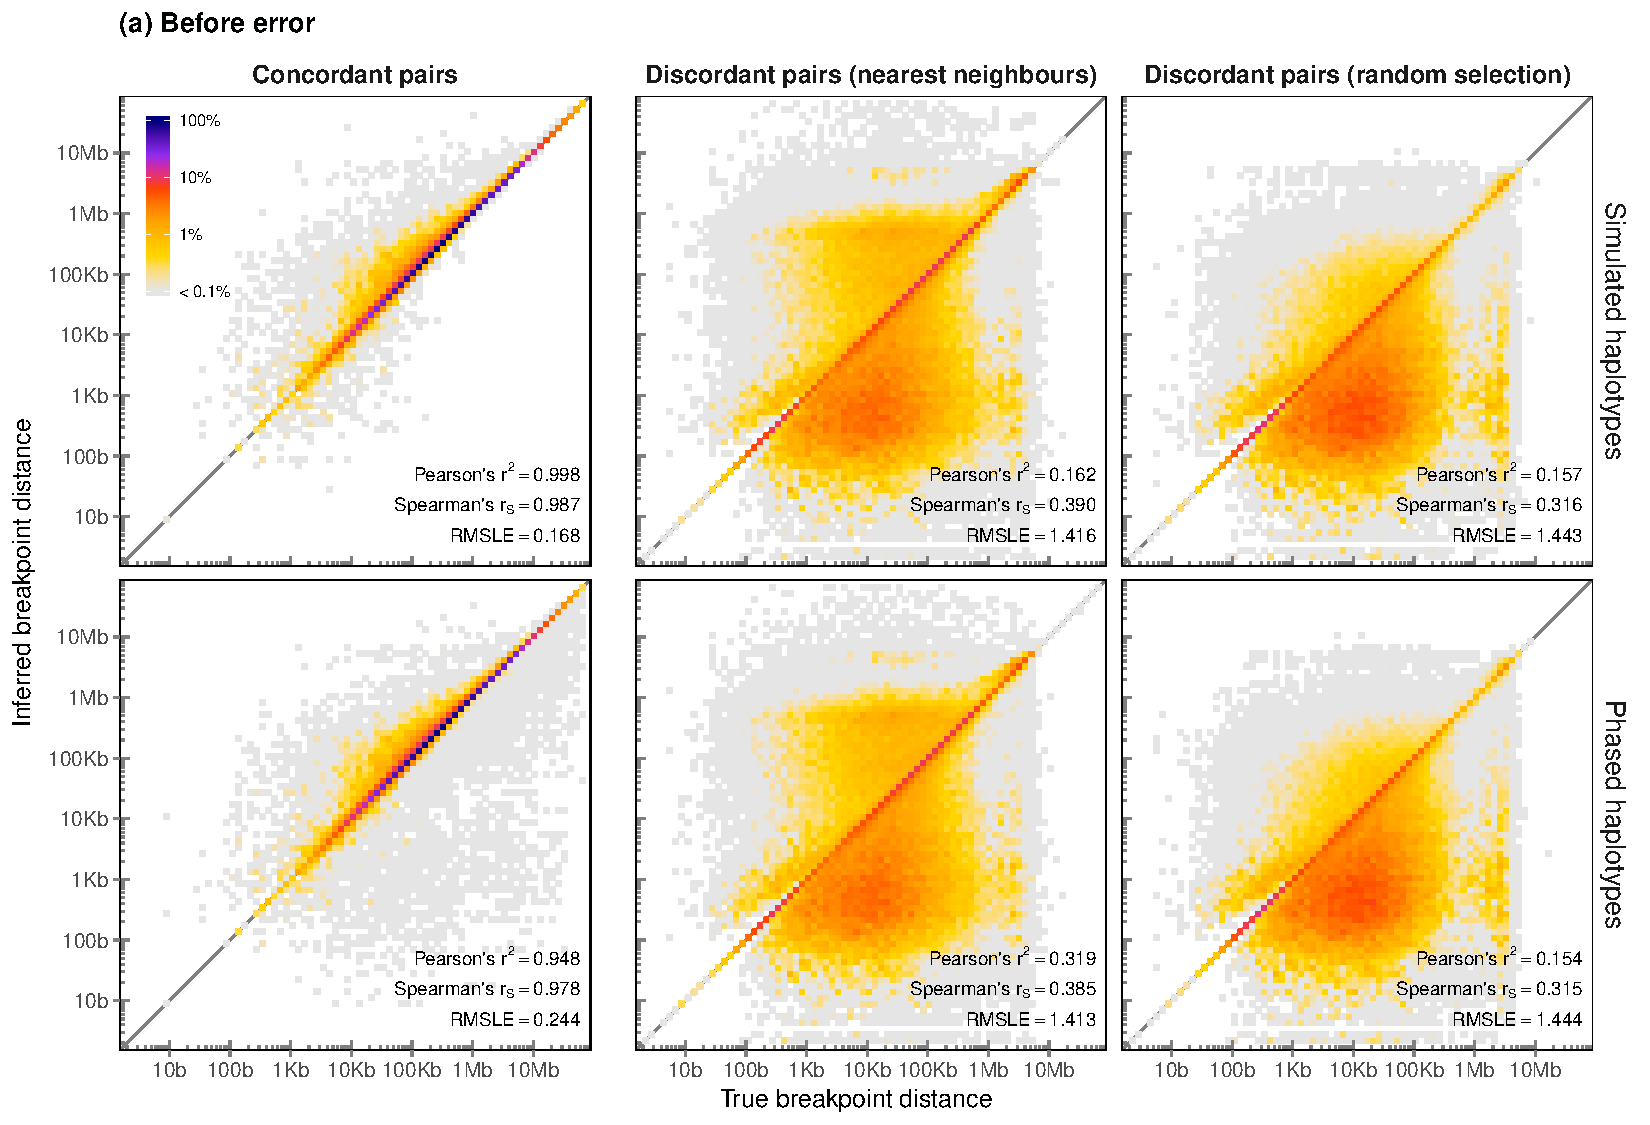
\includegraphics[width=\textwidth]{./img/ch5/hhmm_ibd_rel_A}
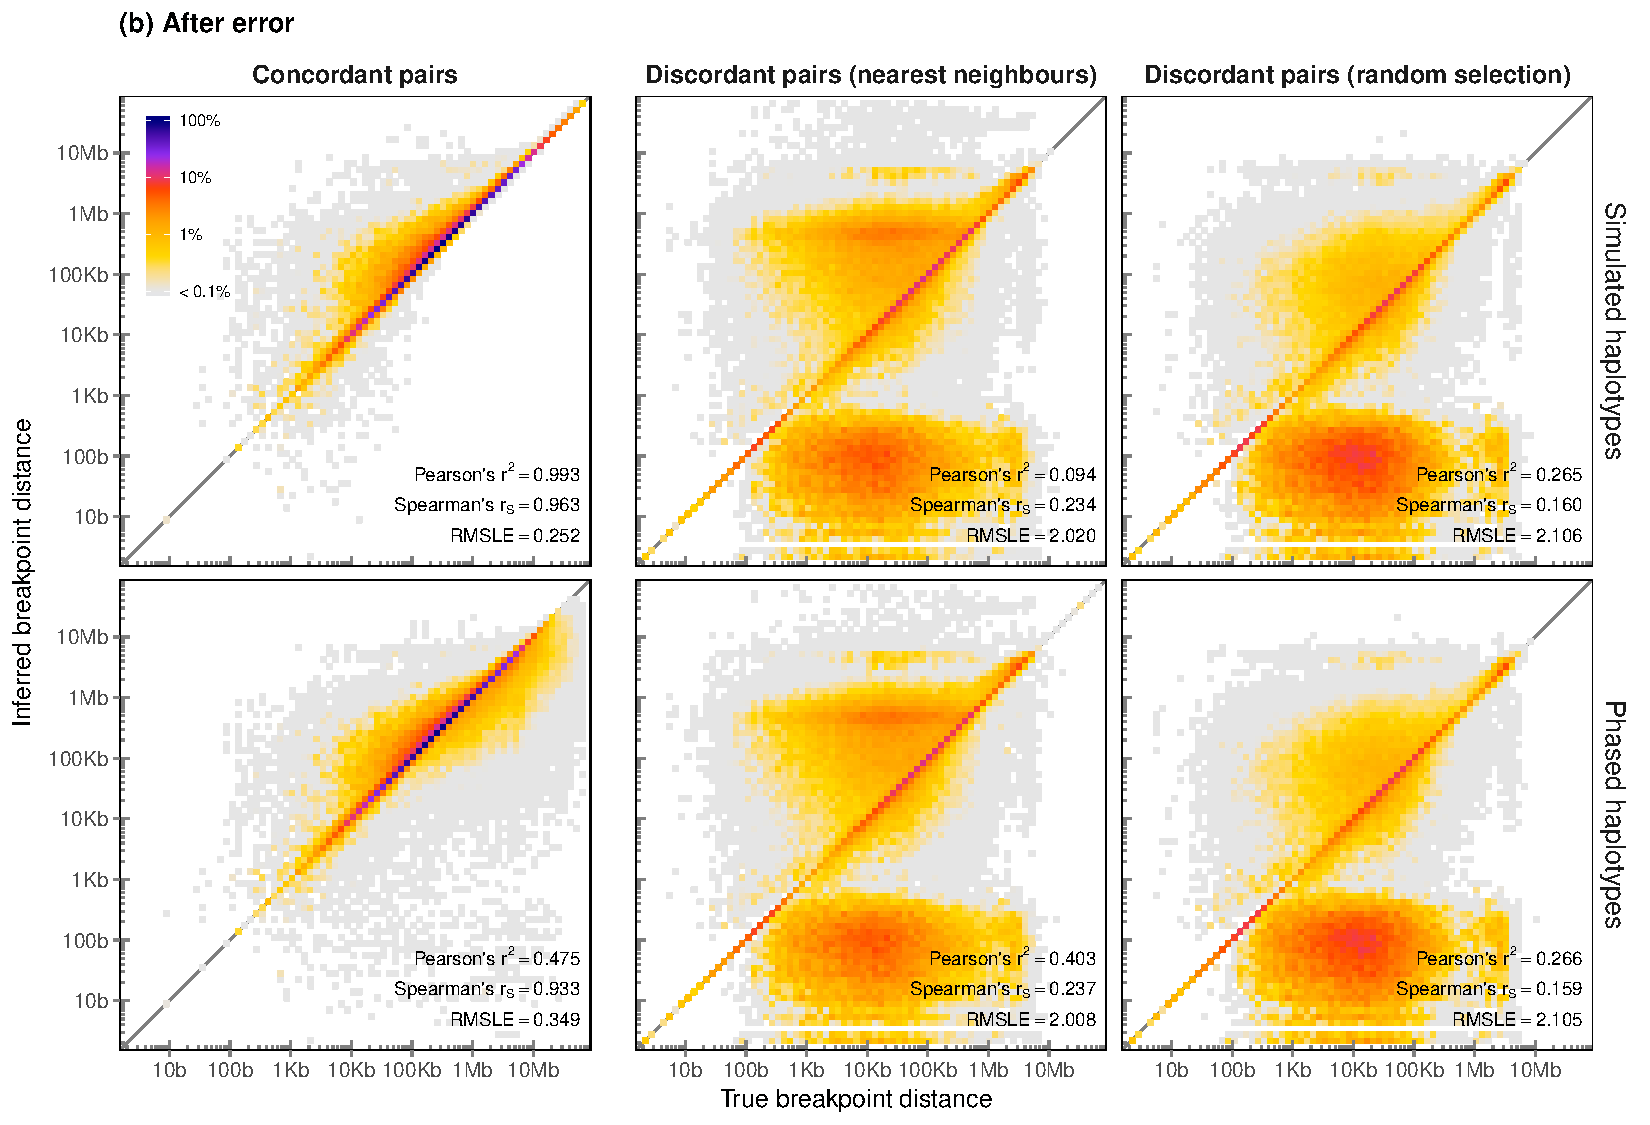
\includegraphics[width=\textwidth]{./img/ch5/hhmm_ibd_rel_B}
\Caption{Density of breakpoint positions inferred using the haplotype-based HMM}
{The physical distance between true and inferred breakpoints (either left or right-hand side) is shown, where colours indicate the maximised density of breakpoints at the relative distance to the focal position, around which a shared haplotype segment was detected.
Pair selection was done using the relaxed nearest neighbour approach and at random.
Note that concordant pairs were selected at random throughout.
Results were obtained on data before \textbf{(a)} and after error \textbf{(b)}, separately on simulated and phased haplotypes.}
{fig:hhmm_ibd_rel}
\end{figure}

%


%
\subsubsection{Shared haplotype inference}
%

In \cpref{fig:hhmm_ibd_rel}, the physical distance between inferred breakpoints and the corresponding focal site is shown relative to the true distance as determined from simulation records.
In the following, the genetic lengths of inferred breakpoint intervals around alleles at a given frequency was used to evaluate the accuracy of the \gls{hmm}; note that boundary cases were removed.
Results are shown in \cpref{fig:hhmm_ibd_len}, for the analysis before and after data error, for analyses on true and phased haplotypes, and for discordant pairs selected as the nearest neighbours or at random.
The summary statistics used to measure accuracy are also given in \cref{fig:hhmm_ibd_len}.


%
% !TEX root = ../../main.tex


\begin{figure}[!htb]
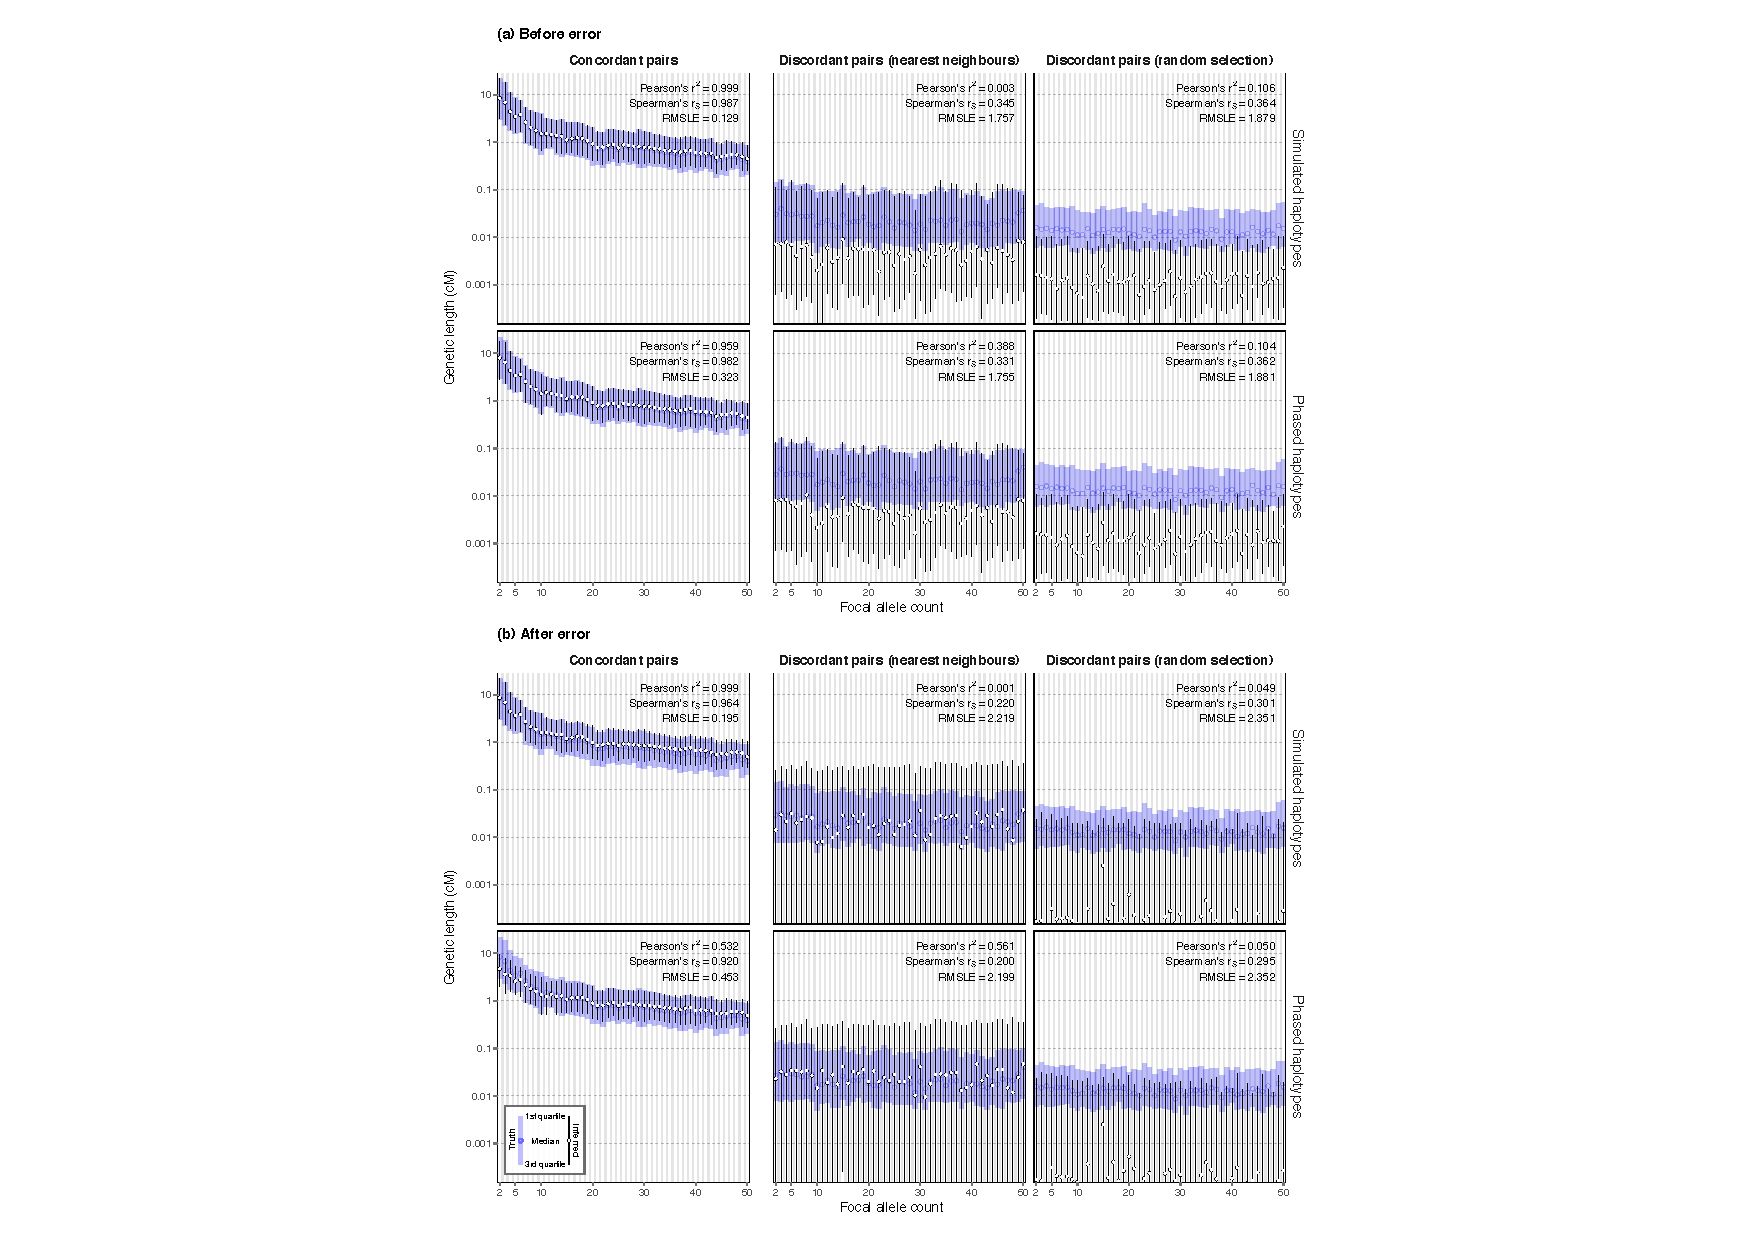
\includegraphics[width=\textwidth]{./img/ch5/hhmm_ibd_len}
\Caption{Genetic length of shared haplotype segments inferred using the haplotype-based HMM}
{The distribution of genetic length is shown by allele count of the focal variant in the simulated sample of ${N=\n{5000}}$ haplotypes, in direct comparison to the corresponding true length at the same set of shared segments (\emph{blue} bars).
This is separately shown for concordant discordant pairs.
Pair selection was done using the relaxed nearest neighbour approach and at random.
Note that concordant pairs were selected at random throughout.
Results were obtained on data before \textbf{(a)} and after error \textbf{(b)}.}
{fig:hhmm_ibd_len}
\end{figure}

%

The accuracy to infer shared haplotype lengths in concordant pairs was high overall.
The impact of phasing error were seen when intervals were relatively long; \eg at \fk{\leq 10}.
At higher frequencies, differences between simulated and phased haplotypes became negligible.
However, intervals showed a tendency to be overestimated towards higher frequency, which was pronounced after error.

In comparison, accuracy of intervals inferred in discordant pairs was low.
While the majority of segments were shorter than those found around concordant pairs, which is expected, inferred lengths were generally underestimated before error.
Notably, median genetic length was longer after error, but at a loss of accuracy; \eg measured using Spearman's rank correlation coefficient ($r_S$) and \glsentryfull{rmsle}.
Also, these metrics did not suggest a notable difference between results obtained on simulated or phased data.

When using the relaxed nearest neighbour approach, median genetic length inferred around selected discordant pairs was longer compared to randomly selected pairs, which suggested that the approach was useful to prioritise the nearest genealogical neighbours in the sample.
However, $r_S$ was reduced when compared to the random selection approach, while lower values of \gls{rmsle} indicated a smaller magnitude of error.



%
\subsubsection{Allele age estimation}
%

The shared haplotypes inferred using the haplotype-based \gls{hmm} were subsequently used to estimate allele age at the selected target sites.
\Cpref{fig:hhmm_age} shows the results obtained when the nearest neighbour approach was used.
Age estimated using the mutation clock (\ClockM), recombination clock (\ClockR), and combined clock (\ClockC) were compared before and after error, and for simulated and phased data.
Summary statistics for both the nearest neighbour and random selection approaches are given in \cpref{tab:stats_hhmm_age}.
Note that ``true'' age was set at $t_m$; \ie the geometric mean between the time of coalescent events below and above the focal mutation event ($t_c$~and~$t_d$), according to which accuracy was measured.

%
% !TEX root = ../../main.tex


\begin{figure}[p]
\centering
\vspace*{-5pt}
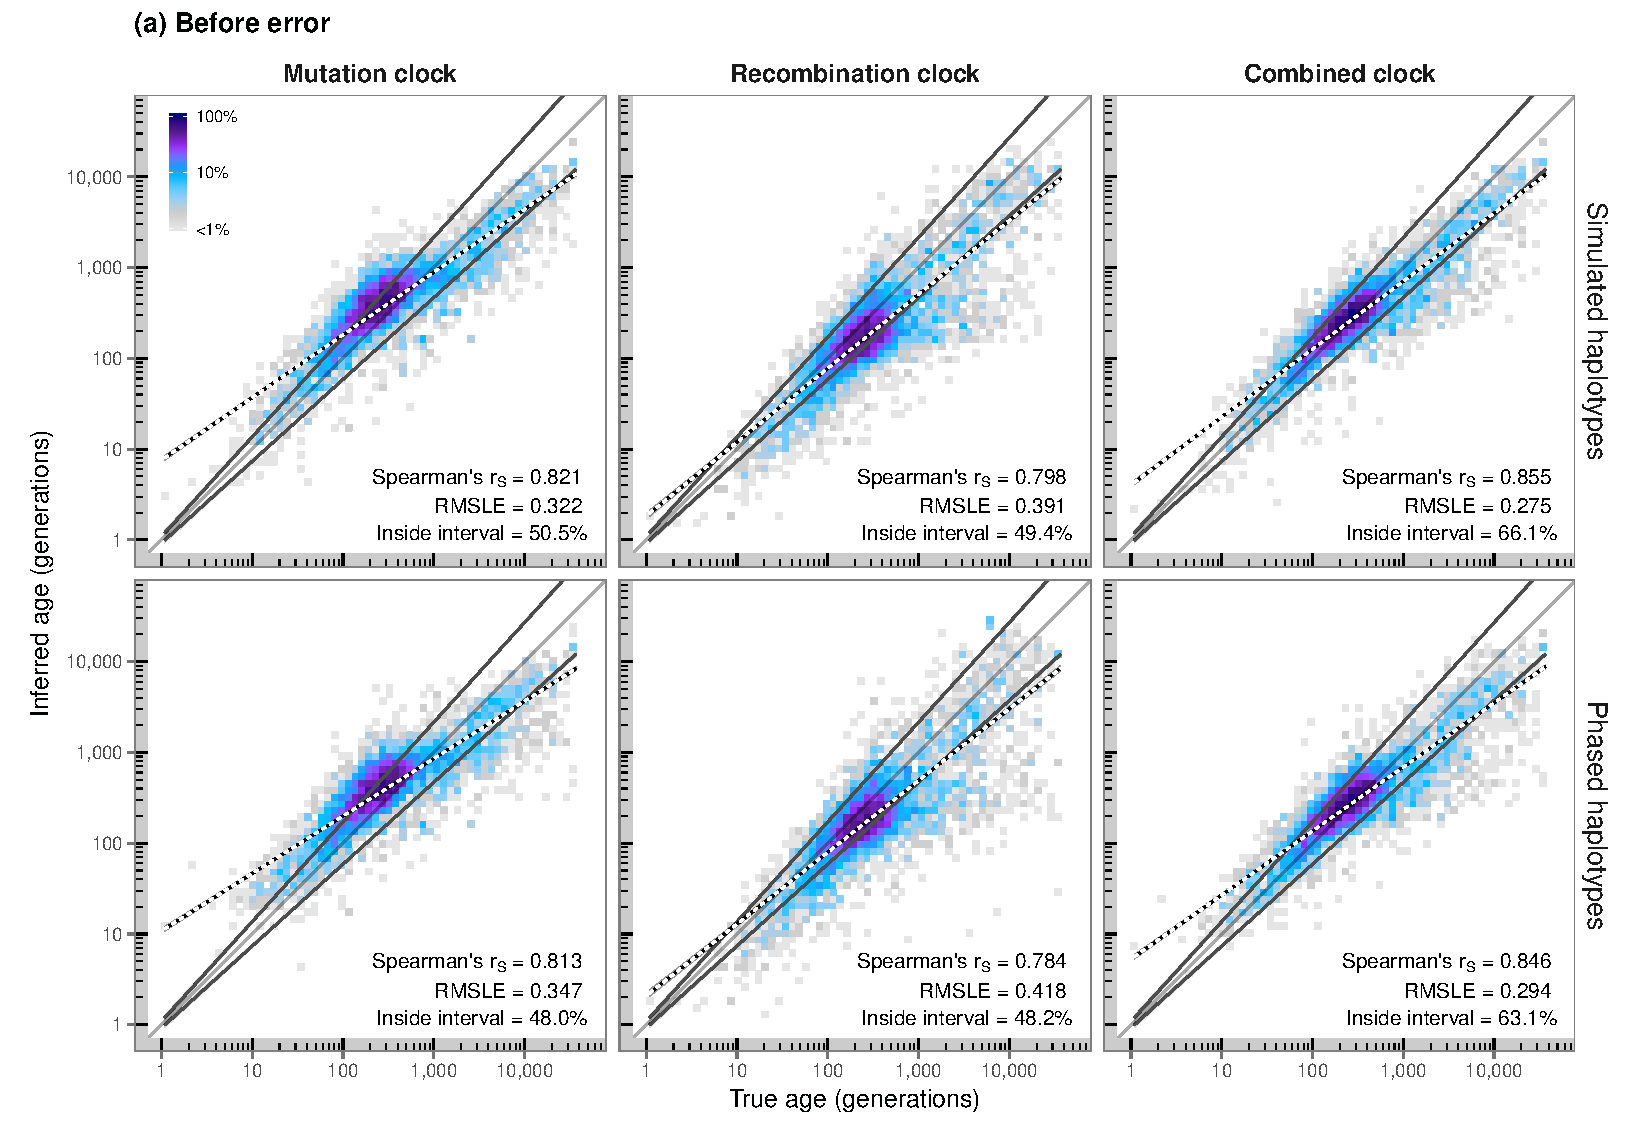
\includegraphics[width=0.95\textwidth]{./img/ch5/hhmm_age_A}
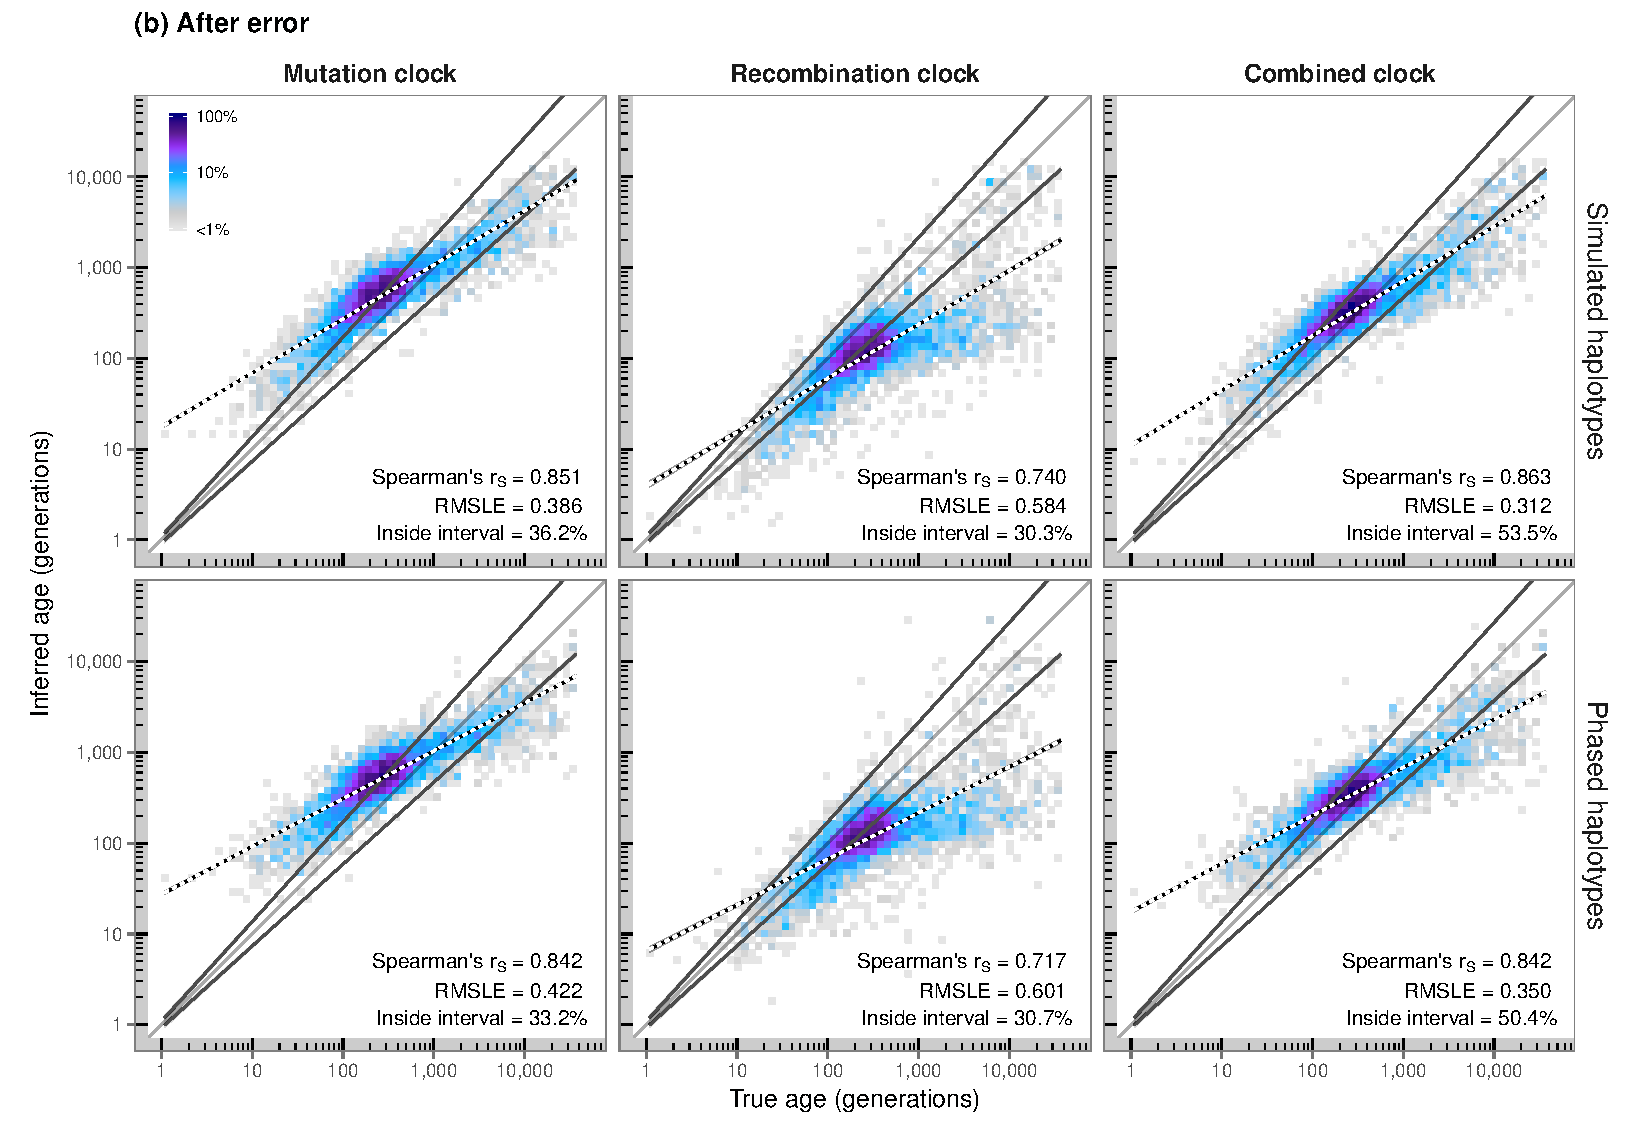
\includegraphics[width=0.95\textwidth]{./img/ch5/hhmm_age_B}
\Caption{Allele age inferred using the haplotype-based HMM}
{The haplotype-based \gls{hmm} was used to infer breakpoint intervals in data before \textbf{(a)} and after error \textbf{(b)}; analyses were conducted on ``true'' (simulated) haplotypes and phased haplotypes.
Age was estimated using each of the \n{3} clock models, for a random set of \n{5000} target sites at \fk{2,50}, for which \n{100} concordant pairs were randomly selected and \n{100} discordant pairs were selected using the relaxed nearest neighbour approach.
Note that ``true'' age was set at $t_m$, according to which the summary metrics shown were calculated.
Regression lines above and below the dividing line indicate $t_c$ and $t_d$.
The \emph{black-white} line shows the regression over age estimates.
Colours indicate the density of true and estimated age; scaled as the maximised density per panel.}
{fig:hhmm_age}
\end{figure}

%

Each clock model was measured at overall high accuracy, both before and after error, but where \ClockC was found to outperform other models throughout.
For example, the proportion of alleles ``correctly'' estimated (such that estimated age was within the interval between $t_c$~and~$t_d$) was highest for \ClockC when the nearest neighbour approach was used, consistently yielding $>50\%$.
The only exception was seen when discordant pairs were selected randomly, where the proportion of correct alleles was higher for \ClockR.
Accuracy was overall lower for \ClockM in each comparison.

%
% !TEX root = ../../main.tex


\begin{table}[!htb]
\Caption{Accuracy of inferred age using the haplotype-based HMM}
{Age was estimated using the mutation clock (\ClockM), recombination clock (\ClockR), and combined clock (\ClockC) based on inference of breakpoint intervals using the haplotype-based \gls{hmm}.
Analyses were conducted on dataset $\mathcal{D}_B$ and $\mathcal{D}_B^{\ast}$ (\ie before and after error), as well as simulated and phased haplotype data in both.
Note that these metrics were calculated with respect to $t_m$; \ie the geometric mean between $t_c$~and~$t_d$.}
{tab:stats_hhmm_age}
\newcommand{\mergerows}[2]{\multirow{#1}{*}{\begin{tabular}[c]{@{}l@{}}#2\end{tabular}}}
\newcommand{\prform}[1]{\num[round-mode=places,round-precision=1]{#1}}
\centering
\begin{tabular}{lc
c
S[table-format=1.3]
S[table-format=1.3]
c
S[table-format=1.3]
S[table-format=1.3]
}
\toprule
\mergerows{2}{Pair \\ selection} &
\mergerows{2}{Clock \\ model} & &
\multicolumn{2}{c}{Before error} & &
\multicolumn{2}{c}{After error} \\
\cmidrule(lr){4-5}
\cmidrule(lr){7-8}
 &  &  &
\mergerows{2}{\textsc{simulated} \\[-0.5ex] \textsc{haplotypes}} &
\mergerows{2}{\textsc{phased} \\[-0.5ex] \textsc{haplotypes}} & &
\mergerows{2}{\textsc{simulated} \\[-0.5ex] \textsc{haplotypes}} &
\mergerows{2}{\textsc{phased} \\[-0.5ex] \textsc{haplotypes}} \\
 & & & & & & & \\
\otoprule
\multicolumn{8}{@{}l}{\,Spearman's rank correlation coefficient ($r_S$)} \\
\midrule
\mergerows{3}{\emph{Nearest} \\ \emph{neighbour}}
 & \ClockM  & &  0.8213762  &  0.8130858   & &   0.8506566  &  0.8423003  \\
 & \ClockR  & &  0.7977185  &  0.7838349   & &   0.7398329  &  0.7171380  \\
 & \ClockC  & &  0.8549228  &  0.8458980   & &   0.8633220  &  0.8421853  \\
\cmidrule(lr){1-8}
\mergerows{3}{\emph{Randomly} \\ \emph{selected}}
 & \ClockM  & &  0.7888687  &  0.7824700   & &   0.8271630  &  0.8261144  \\
 & \ClockR  & &  0.8220781  &  0.8153260   & &   0.7806561  &  0.7805064  \\
 & \ClockC  & &  0.8367566  &  0.8258520   & &   0.8634527  &  0.8491384  \\
\otoprule
\multicolumn{8}{@{}l}{\,\Glsentryfull{rmsle}} \\
\midrule
\mergerows{3}{\emph{Nearest} \\ \emph{neighbour}}
 & \ClockM  & &  0.3222657  &  0.3467713   & &   0.3859870  &  0.4222096  \\
 & \ClockR  & &  0.3914181  &  0.4182889   & &   0.5843978  &  0.6008549  \\
 & \ClockC  & &  0.2749296  &  0.2943302   & &   0.3119283  &  0.3501693  \\
\cmidrule(lr){1-8}
\mergerows{3}{\emph{Randomly} \\ \emph{selected}}
 & \ClockM  & &  0.3893356  &  0.4091920   & &   0.4273054  &  0.4638195  \\
 & \ClockR  & &  0.3231159  &  0.3372835   & &   0.3422211  &  0.3472310  \\
 & \ClockC  & &  0.3109234  &  0.3285661   & &   0.3308763  &  0.3711822  \\
\otoprule
\multicolumn{8}{@{}l}{\,Proportion inside interval (\%)} \\
\midrule
\mergerows{3}{\emph{Nearest} \\ \emph{neighbour}}
 & \ClockM  & &  {\prform{50.48}} & {\prform{48.02}}  & &  {\prform{36.20}}  &  {\prform{33.18}}  \\
 & \ClockR  & &  {\prform{49.38}} & {\prform{48.21}}  & &  {\prform{30.26}}  &  {\prform{30.72}}  \\
 & \ClockC  & &  {\prform{66.08}} & {\prform{63.11}}  & &  {\prform{53.48}}  &  {\prform{50.42}}  \\
\cmidrule(lr){1-8}
\mergerows{3}{\emph{Randomly} \\ \emph{selected}}
 & \ClockM  & &  {\prform{41.54}} & {\prform{38.86}}  & &  {\prform{34.66}}  &  {\prform{31.22}}  \\
 & \ClockR  & &  {\prform{51.10}} & {\prform{50.24}}  & &  {\prform{55.42}}  &  {\prform{54.62}}  \\
 & \ClockC  & &  {\prform{50.78}} & {\prform{48.18}}  & &  {\prform{44.14}}  &  {\prform{40.80}}  \\
\bottomrule
\end{tabular}
\end{table}





% \sisetup{
%     input-open-uncertainty  = ,
%     input-close-uncertainty = ,
%     table-align-text-pre  = false,
%     table-align-text-post = false,
%     round-mode=places,
%     round-precision=3,
%     table-space-text-pre  = {[},
%     table-space-text-post = {]},
% }
%
% \begin{tabular}{lc
% c
% S[table-format=1.3]@{~}
% S[table-format=1.3]
% S[table-format=1.3]@{~}
% S[table-format=1.3]
% c
% S[table-format=1.3]@{~}
% S[table-format=1.3]
% S[table-format=1.3]@{~}
% S[table-format=1.3]
% }
% \toprule
% \mergerows{2}{Pair \\ selection} &
% \mergerows{2}{Clock \\ model} & &
% \multicolumn{4}{c}{Before error} & &
% \multicolumn{4}{c}{After error} \\
% \cmidrule(lr){4-7}
% \cmidrule(lr){9-12}
%  &  &  &
% \multicolumn{2}{c}{\mergerows{2}{\textsc{simulated} \\[-0.5ex] \textsc{haplotypes}}} &
% \multicolumn{2}{c}{\mergerows{2}{\textsc{phased} \\[-0.5ex] \textsc{haplotypes}} } & &
% \multicolumn{2}{c}{\mergerows{2}{\textsc{simulated} \\[-0.5ex] \textsc{haplotypes}}} &
% \multicolumn{2}{c}{\mergerows{2}{\textsc{phased} \\[-0.5ex] \textsc{haplotypes}}} \\
%  & & & & & & & & & & & \\
% \otoprule
% \multicolumn{12}{@{}l}{\,Spearman's rank correlation coefficient ($r_S$)} \\
% \midrule
% \mergerows{3}{\emph{Nearest} \\ \emph{neighbour}}
%  & \ClockM  & &  0.8213762 & [0.8043555]  &  0.8130858 & [0.7889697]   & &   0.8506566 & [0.8472187]  &  0.8423003 & [0.8344553]  \\
%  & \ClockR  & &  0.7977185 & [0.7802489]  &  0.7838349 & [0.7570393]   & &   0.7398329 & [0.7319917]  &  0.7171380 & [0.7201037]  \\
%  & \ClockC  & &  0.8549228 & [0.8425151]  &  0.8458980 & [0.8254148]   & &   0.8633220 & [0.8702781]  &  0.8421853 & [0.8480484]  \\
% \cmidrule(lr){1-12}
% \mergerows{3}{\emph{Randomly} \\ \emph{selected}}
%  & \ClockM  & &  0.7888687 & [0.7827576]  &  0.7824700 & [0.7707588]   & &   0.8271630 & [0.8248231]  &  0.8261144 & [0.8153433]  \\
%  & \ClockR  & &  0.8220781 & [0.7930409]  &  0.8153260 & [0.7808431]   & &   0.7806561 & [0.7730264]  &  0.7805064 & [0.7676446]  \\
%  & \ClockC  & &  0.8367566 & [0.8281091]  &  0.8258520 & [0.8103608]   & &   0.8634527 & [0.8604035]  &  0.8491384 & [0.8385275]  \\
% \otoprule
% \multicolumn{12}{@{}l}{\,\Glsentryfull{rmsle}} \\
% \midrule
% \mergerows{3}{\emph{Nearest} \\ \emph{neighbour}}
%  & \ClockM  & &  0.3222657 & [0.3498267]  &  0.3467713 & [0.3765934]   & &   0.3859870 & [0.3896325]  &  0.4222096 & [0.4295211]  \\
%  & \ClockR  & &  0.3914181 & [0.3637233]  &  0.4182889 & [0.3995065]   & &   0.5843978 & [0.4291032]  &  0.6008549 & [0.4402350]  \\
%  & \ClockC  & &  0.2749296 & [0.2810064]  &  0.2943302 & [0.3175376]   & &   0.3119283 & [0.2995877]  &  0.3501693 & [0.3465771]  \\
% \cmidrule(lr){1-12}
% \mergerows{3}{\emph{Randomly} \\ \emph{selected}}
%  & \ClockM  & &  0.3893356 & [0.4020786]  &  0.4091920 & [0.4247604]   & &   0.4273054 & [0.4309427]  &  0.4638195 & [0.4718083]  \\
%  & \ClockR  & &  0.3231159 & [0.3854742]  &  0.3372835 & [0.4075467]   & &   0.3422211 & [0.3553941]  &  0.3472310 & [0.3872206]  \\
%  & \ClockC  & &  0.3109234 & [0.3257049]  &  0.3285661 & [0.3529276]   & &   0.3308763 & [0.3322117]  &  0.3711822 & [0.3878792]  \\
% \otoprule
% \multicolumn{12}{@{}l}{\,Proportion inside interval (\%)} \\
% \midrule
% \mergerows{3}{\emph{Nearest} \\ \emph{neighbour}}
%  & \ClockM  & &  {\prform{50.48}} & {[\prform{48.80}]} & {\prform{48.02}} & {[\prform{46.40}]}  & &  {\prform{36.20}} & {[\prform{36.68}]}  &  {\prform{33.18}} & {[\prform{33.80}]}  \\
%  & \ClockR  & &  {\prform{49.38}} & {[\prform{49.58}]} & {\prform{48.21}} & {[\prform{48.78}]}  & &  {\prform{30.26}} & {[\prform{45.36}]}  &  {\prform{30.72}} & {[\prform{46.84}]}  \\
%  & \ClockC  & &  {\prform{66.08}} & {[\prform{63.60}]} & {\prform{63.11}} & {[\prform{60.34}]}  & &  {\prform{53.48}} & {[\prform{54.26}]}  &  {\prform{50.42}} & {[\prform{50.48}]}  \\
% \cmidrule(lr){1-12}
% \mergerows{3}{\emph{Randomly} \\ \emph{selected}}
%  & \ClockM  & &  {\prform{41.54}} & {[\prform{41.12}]} & {\prform{38.86}} & {[\prform{38.54}]}  & &  {\prform{34.66}} & {[\prform{34.78}]}  &  {\prform{31.22}} & {[\prform{31.64}]}  \\
%  & \ClockR  & &  {\prform{51.10}} & {[\prform{46.04}]} & {\prform{50.24}} & {[\prform{45.02}]}  & &  {\prform{55.42}} & {[\prform{52.40}]}  &  {\prform{54.62}} & {[\prform{50.44}]}  \\
%  & \ClockC  & &  {\prform{50.78}} & {[\prform{50.00}]} & {\prform{48.18}} & {[\prform{47.58}]}  & &  {\prform{44.14}} & {[\prform{44.54}]}  &  {\prform{40.80}} & {[\prform{41.42}]}  \\
% \bottomrule
% \end{tabular}
%
% \begin{tablenotes}[para,flushleft]\footnotesize
% 	Summary metrics are given for allele age computed as the \emph{raw} (unfiltered) inference together with the corresponding \emph{adjusted} (filtered) inference, where the latter is written with [square brackets].
% \end{tablenotes}

%

%
\subsubsection{Discussion}
%

The results presented in this section indicate a substantial advancement over previously evaluated methods that were employed in the age estimation method.
In particular, the previous genotype-based \gls{hmm} was outperformed, such that it now can be expected that the method can be applied to real data in a reliable way.

However, it would be useful to compare this method to other, established approaches.
For this purpose, in the following section, I used the \glsentryfull{psmc} to infer the \gls{tmrca} at concordant and discordant pairs, from which I derived a posterior distribution that was implemented as described for the \gls{ccf} in \cpref{sec:comp_post_detail} to estimate allele age.



%
\subsection{Comparison to the Pairwise Sequentially Markovian Coalescent (PSMC)}
\label{sec:psmc_eval}
%

The \gls{psmc} model was proposed by \citet{Li:2011ez} to infer historic changes of human population size back in time, using sequence data from \n{2} haplotypes alone (\ie~\n{1} diploid genome).
The model is based on the \gls{smc} introduced and further developed by \citet{McVean:2005ho} and \citet{marjoram2006fast} for an analytically tractable approximation to the \gls{arg} in model-based inferences.
\Citet{Li:2011ez} used the \Gls{psmc} model in \gls{hmm} methods for inference of the \gls{tmrca} between \n{2} haplotypes at sites observed along the pairwise sequence, where the observation states are defined as \texttt{`0'}~(homozygous), \texttt{`1'}~(heterozygous), and \texttt{`$\cdot$'}~(missed) genotypes (\ie allelic pairs).
In particular, coalescent time is divided into discrete intervals, which are the hidden states of the \gls{hmm}, and a posterior probability is obtained for each state using the forward-backward algorithm \citep[\eg, see][]{Rabiner:1989hs}.

I used the PSMC-HMM as a method to infer the \gls{tmrca} of concordant and discordant pairs in the estimation of allele age.
For a given pair, I extracted the computed coalescent time posteriors at a focal position, which I then used in the same way as the posteriors obtained through a ``clock'' model in the \glsentryfull{ccf}, so as to compute the composite posterior distribution at discrete time intervals for subsequent age estimation.

I describe the PSMC-based procedure in the section below.
This is followed by an analysis using the \gls{psmc} method for comparisons to the clock models implemented in \texttt{rvage}, where accuracy was compared in terms of the inferred \gls{tmrca} and allele age.


%
\subsubsection{Implementation to estimate allele age}
%


To establish a baseline comparison with the haplotype-based \gls{hmm} presented here, I first performed the analysis using \texttt{rvage} in which concordant and discordant pairs were selected randomly.
Identical sets of pairs per target site were then analysed using the PSMC-based method.

Note that time intervals in \gls{psmc} are not scaled on a strict logarithmic scale.
The boundaries of intervals are calculated as
\begin{equation}
	t_i~=~0.1\times\euler{\frac{i}{n}\log(1 + 10  T_{\max})}-0.1
\end{equation}
where $T_{\max}$ is the maximum \gls{tmrca} considered (scaled in units of $2\Ne$), $n$ is the number of intervals (\ie hidden states), and ${i=0,1,\ldots,n}$.
Here, I performed the analysis with 64 coalescent time intervals, from which I computed the composite posterior at the mean between consecutive boundaries.

To conduct the analysis, I modified the \texttt{decode} algorithm implemented in software available for the \gls{msmc} method \citep{schiffels2014inferring}, written in \texttt{D}, as it specifically applies the PSMC-HMM when \n{2} haplotype sequences are provided as input data.
Modifications of \texttt{decode} were made to include the option to only return posterior probabilities at a specified target position (without affecting the computation of posteriors).\footnote{Modified \texttt{decode} algorithm: \url{https://github.com/pkalbers/msmc2} \accessed{2017}{11}{04}}

The above modification facilitated faster computations such that I was able to obtain posterior probability distributions for a reasonably large set of target sites for a relatively large number of haplotype pairs.
Yet, it must be noted that \gls{psmc} (as implemented in \texttt{decode} and embedded in the analytical pipeline used here) is slow in comparison to the haplotype-based \gls{hmm} in \texttt{rvage}, which is why such analyses on a larger scale would be computationally prohibitive.

Dataset $\mathcal{D}_A$ was used (${\Ne=\num{10000}}$; ${\mu=\num{1e-08}}$; ${\rho=\num{1e-08}}$; ${N=\num{1000}}$), in which I selected \n{1000} target sites at random at \fk{\geq2} and allele frequency below 50\%, so as to include alleles that could be relatively old (as opposed to only selecting rare alleles that are presumed to be relatively young).
At each site, a maximum of \n{100} concordant and \n{100} discordant pairs was selected, yielding \n{187420} pairwise analyses in total.
The same parameters used for simulating the data were specified for inference in \texttt{rvage} and \gls{psmc}.


%
\subsubsection{Results for the T\textsubscript{MRCA}}
%

Simulation records were scanned to obtain the true \gls{tmrca} for each haplotype pair at a given target site.
The true time of coalescent events was compared to point estimates taken at the median of posterior distributions.
% in \gls{psmc}, but the median of the \gls{ccf} in each clock model.
The median was chosen because the Gamma distribution used to compute posteriors in the clock models may equal zero at the mode, such that the median was seen as a more reliable estimate.
Results for concordant and discordant pairs are shown in \cpref{fig:psmc_tmrca}.

%
% !TEX root = ../../main.tex


\begin{figure}[p]
\centering
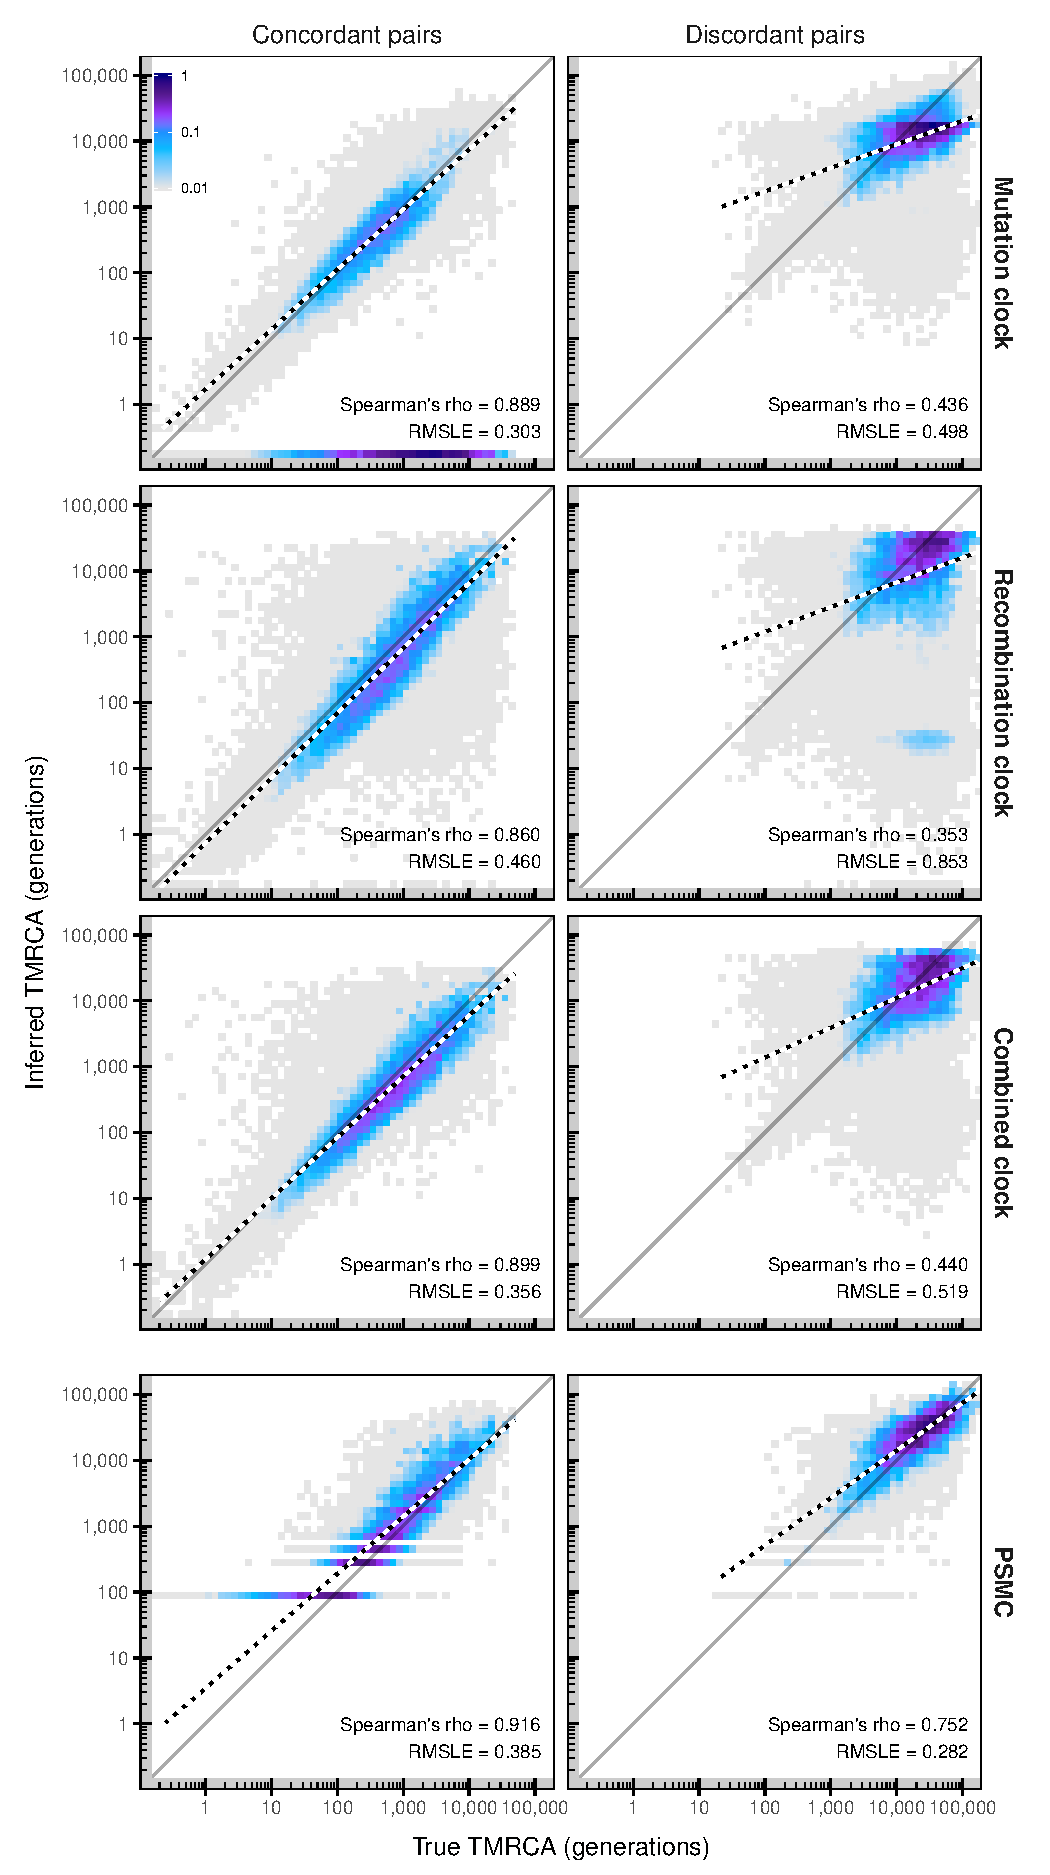
\includegraphics[width=0.8\textwidth]{./img/ch5/psmc_tmrca}
\Caption{True and estimated T\textsubscript{MRCA} using different methods}%
{...}%
{fig:psmc_tmrca}
\end{figure}

%

The combined clock, \ClockC, showed the highest accuracy overall among the clock models when concordant pairs were considered; measured using rank correlation ($r_S$) and \glsentryfull{rmsle}.
The mutation clock, \ClockM, was slightly more accurate for discordant pairs.
The PSMC-based approach, however, was highest in terms of $r_S$ in both concordant and discordant pairs, but where \gls{rmsle} indicated a higher magnitude of error compared to \ClockC and \ClockM.
Notably, as seen in \cref{fig:psmc_tmrca}, because of the discrete time intervals in \gls{psmc} it was problematic to infer recent \gls{tmrca}.
While it would be possible to increase the number of hidden states to include intervals at more recent points in time, a consequence would be that computations would become substantially slower.

%
% !TEX root = ../../main.tex


\begin{table}[!htb]
\Caption{Accuracy of T\textsubscript{MRCA} estimation for different methods}
{The \gls{tmrca} estimation conducted using \texttt{PSMC} is compared to estimates obtained using the mutation clock (\ClockM), recombination clock (\ClockR), and combined clock (\ClockC), where estimates were obtained on identical target sites and haplotype pairs.
Accuracy was measured using Spearman's rank correlation coefficient ($r_S$) and root mean squared $\log_{10}$ error ($\rmsle$) at discrete time intervals defined on the true \gls{tmrca} ($t$) of a given pair at a target site, as determined from simulation records.
The number of estimates at a given time interval is indicated ($n$).}
{tab:stats_psmc_tmrca}
\centering
\begin{tabular}{c
r
@{\quad}c
*4{@{\quad}S[table-format=1.3,table-space-text-pre={}]}
@{\quad}c
*4{@{\quad}S[table-format=1.3,table-space-text-pre={}]}}
\toprule
True T\textsubscript{MRCA} & $n$ & &
\multicolumn{4}{c}{Rank correlation ($r_S$)} & &
\multicolumn{4}{c}{$\rmsle$} \\
\cmidrule(lr){4-7}
\cmidrule(lr){9-12}
 (generations) & & &
{\ClockM} & {\ClockR} & {\ClockC} & {\texttt{PSMC}} & &
{\ClockM} & {\ClockR} & {\ClockC} & {\texttt{PSMC}} \\
\otoprule
\multicolumn{12}{@{}l}{\,Concordant pairs} \\
\midrule
 \smaller $t\leq\num{100}$                & \n{21384} & &  \bfseries 0.7523226 & 0.6508665 & 0.7285282 & 0.2985932  & &  \bfseries 0.2887397 & 0.4868986 & 0.3874829 & 0.6122015 \\
 \smaller $\num{100}<t\leq\num{1000}$     & \n{69903} & &  0.6933208 & 0.6279257 & 0.7068744 & \bfseries 0.7228590  & &  \bfseries 0.2787932 & 0.4446835 & 0.3338086 & 0.3457944 \\
 \smaller $\num{1000}<t\leq\num{10000}$   & \n{64779} & &  0.5535656 & 0.5813404 & 0.6393111 & \bfseries 0.6643521  & &  0.3555674 & 0.4474132 & 0.3561629 & \bfseries 0.3380173 \\
 \smaller $\num{10000}<t\leq\num{100000}$ &  \n{7322} & &  0.2852226 & 0.2695854 & 0.3372834 & \bfseries 0.5284954  & &  0.4043726 & 0.6017576 & 0.4577933 & \bfseries 0.2412933 \\
 \smaller $t>\num{100000}$                &         0 & &       {--} &      {--} &      {--} &      {--}  & &       {--} &      {--} &      {--} &      {--} \\
\otoprule
\multicolumn{12}{@{}l}{\,Discordant pairs} \\
\midrule
 \smaller $t\leq\num{100}$                & \n{163}    & &  0.0030162 &-0.0050964 & 0.0026681 & \bfseries 0.3281581  & & 1.4952399 & 1.5684122 & 1.5933532 & \bfseries 0.2319879 \\
 \smaller $\num{100}<t\leq\num{1000}$     & \n{2877}   & &  0.2187866 & 0.1950644 & 0.2093315 & \bfseries 0.7086547  & & 0.9202619 & 1.0154081 & 1.0172096 & \bfseries 0.4507880 \\
 \smaller $\num{1000}<t\leq\num{10000}$   & \n{43243}  & &  0.2891992 & 0.2420041 & 0.2930032 & \bfseries 0.5340098  & & 0.4168119 & 0.6868658 & 0.5192949 & \bfseries 0.4065983 \\
 \smaller $\num{10000}<t\leq\num{100000}$ & \n{149683} & &  0.2513271 & 0.2024518 & 0.2614567 & \bfseries 0.5971780  & & 0.4942267 & 0.8817960 & 0.4959336 & \bfseries 0.2271959 \\
 \smaller $t>\num{100000}$                & \n{33070}  & &  0.2417831 & 0.2673083 & \bfseries 0.3145942 & 0.2444100  & & 0.8711090 & 1.1889489 & 0.7198778 & \bfseries 0.3136247 \\
\bottomrule
\end{tabular}
\end{table}

%

An additional analysis was conducted using the results obtained above by sorting pairs by their true \gls{tmrca} into broader time intervals at which accuracy was measured ($r_S$~and~\gls{rmsle}).
The results are given in \cpref{tab:stats_psmc_tmrca}.
The PSMC-HMM was notably more accurate compared to each clock model when discordant pairs where considered.
But for concordant pairs, \ClockC outperformed \gls{psmc} when the true coalescent time was more recent that \n{10000} generations.



%
\subsubsection{Results for allele age}
%

Next, allele age was estimated by calculating the composite posterior distribution from the \gls{tmrca} posteriors obtained in pairwise analyses per approach.
The mode of the resulting composite posterior was taken as a point estimate for allele age.
Results are shown in \cpref{fig:psmc_age}, in which the relevant summary statistics to quantify accuracy are indicated; that is, $r_S$, \gls{rmsle}, and the proportion of ``correct'' alleles (estimated to sit between $t_c$~and~$t_d$).
As before, ``true'' age was set at $t_m$ (geometric mean between $t_c$~and~$t_d$).

%
% !TEX root = ../../main.tex


\begin{figure}[!htb]
\centering
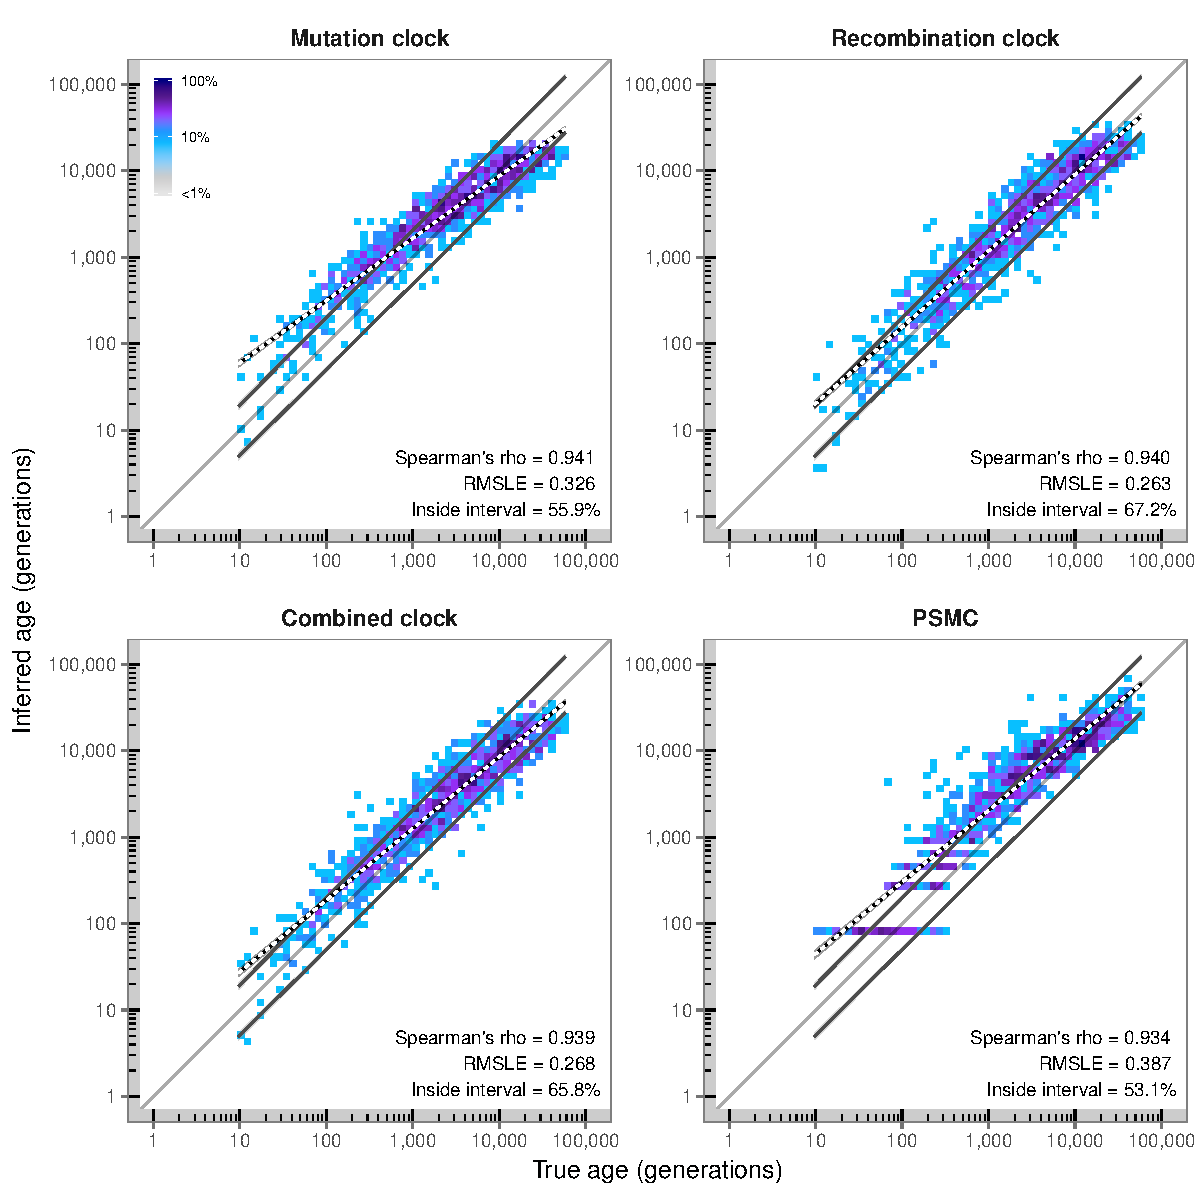
\includegraphics[width=0.9\textwidth]{./img/ch5/psmc_age}
\Caption{Allele age inferred using PSMC}%
{The \n{3} clock models (\ClockM, \ClockR, and \ClockC) were compared to \gls{psmc}.
Posterior distributions obtained on the same set of concordant and discordant pairs were used to compute the composite posterior distribution, from which point estimates were taken at the mode in each approach.
The results shown compare the ``true'' age of an allele (set at $t_m$) to the estimated age at \n{1000} target sites in dataset $\mathcal{D}_A$, which were randomly selected at allele frequency $\leq 50\%$.
Regression lines above and below the dividing line indicate the regression over $t_c$ and $t_d$.
The \emph{black-white} line shows the regression over age estimates.
Colours indicate the density of true and estimated age; scaled as the maximised density.}
{fig:psmc_age}
\end{figure}

%

Each method achieved high levels of accuracy overall; for example, ${r_S>0.9}$ in each method.
The proportion of correctly estimated alleles was $>65\%$ in \ClockR and \ClockC.
However, rank correlation measured for the PSMC-based approach was lowest in this comparison.
Likewise, \gls{rmsle} indicated a higher magnitude of error for \gls{psmc}, and the proportion of correct alleles was also smaller.

Additionally, these results were again sorted into broader time intervals.
Three intervals were distinguished at a nominal value of \n{1000}~generations, so as to distinguish relatively ``young'' alleles from ``old'' ones, considering that the distribution of true allele age was defined at overlapping age intervals at $t_c$~and~$t_d$.
Exact definitions and accuracy results are given in \cpref{tab:stats_psmc_age}.
Notably, rank correlation measured at alleles estimated based on \gls{psmc} was highest for older alleles, but where $r_S$ was higher for \ClockM when younger alleles were considered.
The proportion of correct alleles and the magnitude of error, however, favoured \ClockR and \ClockC overall.

%
% !TEX root = ../../main.tex


\begin{table}[!htb]
\Caption{Accuracy of age inference for different methods}
{...}
{tab:stats_psmc_age}
\centering
\begin{threeparttable}
\begin{tabular}{c
@{\quad}c
*3{S[table-format=1.3]}
@{\quad}c
*3{S[table-format=1.3]}
@{\quad}c
*3{S[table-format=2.1,round-precision=1]}}
\toprule
Method & &
\multicolumn{3}{c}{Rank correlation ($r_S$)} & &
\multicolumn{3}{c}{$\rmsle$} & &
\multicolumn{3}{c}{Inside interval (\%)} \\
\cmidrule(lr){3-5}
\cmidrule(lr){7-9}
\cmidrule(lr){11-13}
 & &
 {Set A} & {Set B} & {Set C} & &
 {Set A} & {Set B} & {Set C} & &
 {Set A} & {Set B} & {Set C} \\
\otoprule
\ClockM       & & \bfseries 0.888434 & 0.671322 & 0.791078 & & 0.477437 & 0.296484 & 0.249119 & & 23.6051 & 66.9642 & 65.1933 \\
\ClockR       & & 0.839882 & 0.673469 & 0.802052 & & \bfseries 0.306607 & 0.272292 & \bfseries 0.238252 & & \bfseries 53.2188 & \bfseries 82.5892 & 66.8508 \\
\ClockC       & & 0.853531 & 0.675706 & 0.800950 & & 0.332719 & \bfseries 0.262146 & 0.238445 & & 45.9227 & 81.6964 & \bfseries 67.7716 \\
\texttt{PSMC} & & 0.817085 & \bfseries 0.747075 & \bfseries 0.828317 & & 0.525377 & 0.443703 & 0.276726 & & 30.9012 & 55.8558 & 61.5101 \\
\bottomrule
\end{tabular}
\begin{tablenotes}\footnotesize
	\item Set~A: ~ ``Young'' age, $n=233$, selected at ${t_d \leq \num{1000}}$
  \item Set~B: ~ ``Intermediate'' age, $n=222$, selected at ${t_c < \num{1000}, ~ t_d > \num{1000}}$
  \item Set~C: ~ ``Old'' age, $n=543$, selected at ${t_c \geq \num{1000}}$
\end{tablenotes}
\end{threeparttable}
\end{table}

%


%
\subsubsection{Discussion}
%

Allele age estimated using \ClockM, \ClockR, or \ClockC was overall comparable to the estimates obtained using the PSMC-based approach.
However, it must be noted that the integration of \gls{psmc} as a method to subsequently arrive at the composite posterior distribution may not have been an ideal baseline for comparisons to the clock models developed in this chapter.
In particular, the current procedure considered 64 coalescent time intervals, which may not directly compare to the continuous scale used by the estimation method.

Nonetheless, the results presented in this section suggested that the haplotype-based \gls{hmm} used for targeted shared haplotype inference achieved comparable estimates of \gls{tmrca}, despite incorporating a (biased) empirical emission model.
I further showed that the haplotype-based \gls{hmm} was able to estimate age of alleles that occurred at relatively high frequencies in the data.
Also, note that the decreased accuracy in inferences at discordant pairs had only minor effects on subsequent estimation of allele age.
Thus, I used the haplotype-based \gls{hmm} in the following section to estimate allele age in real data.





%
\subsection{Allele age estimation in 1000 Genomes}\label{sec:hhmm_1kg}
%

The haplotype-based \gls{hmm} was used for allele age estimation in an extensive analysis of data from the \glsentryfull{1kg} Phase~\rom{3}.
I selected \n{50000} sites at random in chromosomes~1-22, but only at positions within high confidence regions as defined in the strict accessibility mask available for the Phase~\rom{3} dataset.
The diploid sample size was ${N=\num{2504}}$.
Note that all sites at \fk{\geq 2} were considered.
Model parameters in \texttt{rvage} were ${\Ne=\n{10000}}$, ${\mu=\num[round-precision=1]{1.2e-8}}$, and recombination rates according to genetic maps available from \gls{hapmap} Phase~\rom{2}, Build~37.\footnote{HapMap recombination map: \url{ftp://ftp.ncbi.nlm.nih.gov//hapmap/recombination/2011-01_phaseII_B37/genetic_map_HapMapII_GRCh37.tar.gz} \accessed{2016}{11}{12}}

In total, \dec{2.370018}~million concordant and \dec{5.204300}~million discordant pairs were analysed.
Below, I provide a descriptive analysis of the haplotype structure at alleles shared within and between populations, followed by an overview of allele age as estimated per population group; namely African~(AFR), Ad-Mixed American~(AMR), East~Asian~(EAS), European~(EUR), and South~Asian~(SAS).
I conclude this section with selected examples where allele age was estimated at specific loci.


%
\subsubsection{Shared haplotypes inferred by population}
%

The set of pairs was divided into pairs at which the focal allele was shared among the individuals within the same population and those at which it was shared between different groups.
This implied that only concordant pairs were considered, of which \dec{2.357372}~million were retained after removing boundary cases.
Median physical and genetic lengths are shown in \cpref{fig:1KG20_pop_len_hhmm}; the proportion of pairs at which alleles were shared within and between populations is indicated.

%
%!TEX root = ../../main.tex


\begin{figure}[p]
\centering
\makebox[\textwidth][c]{%
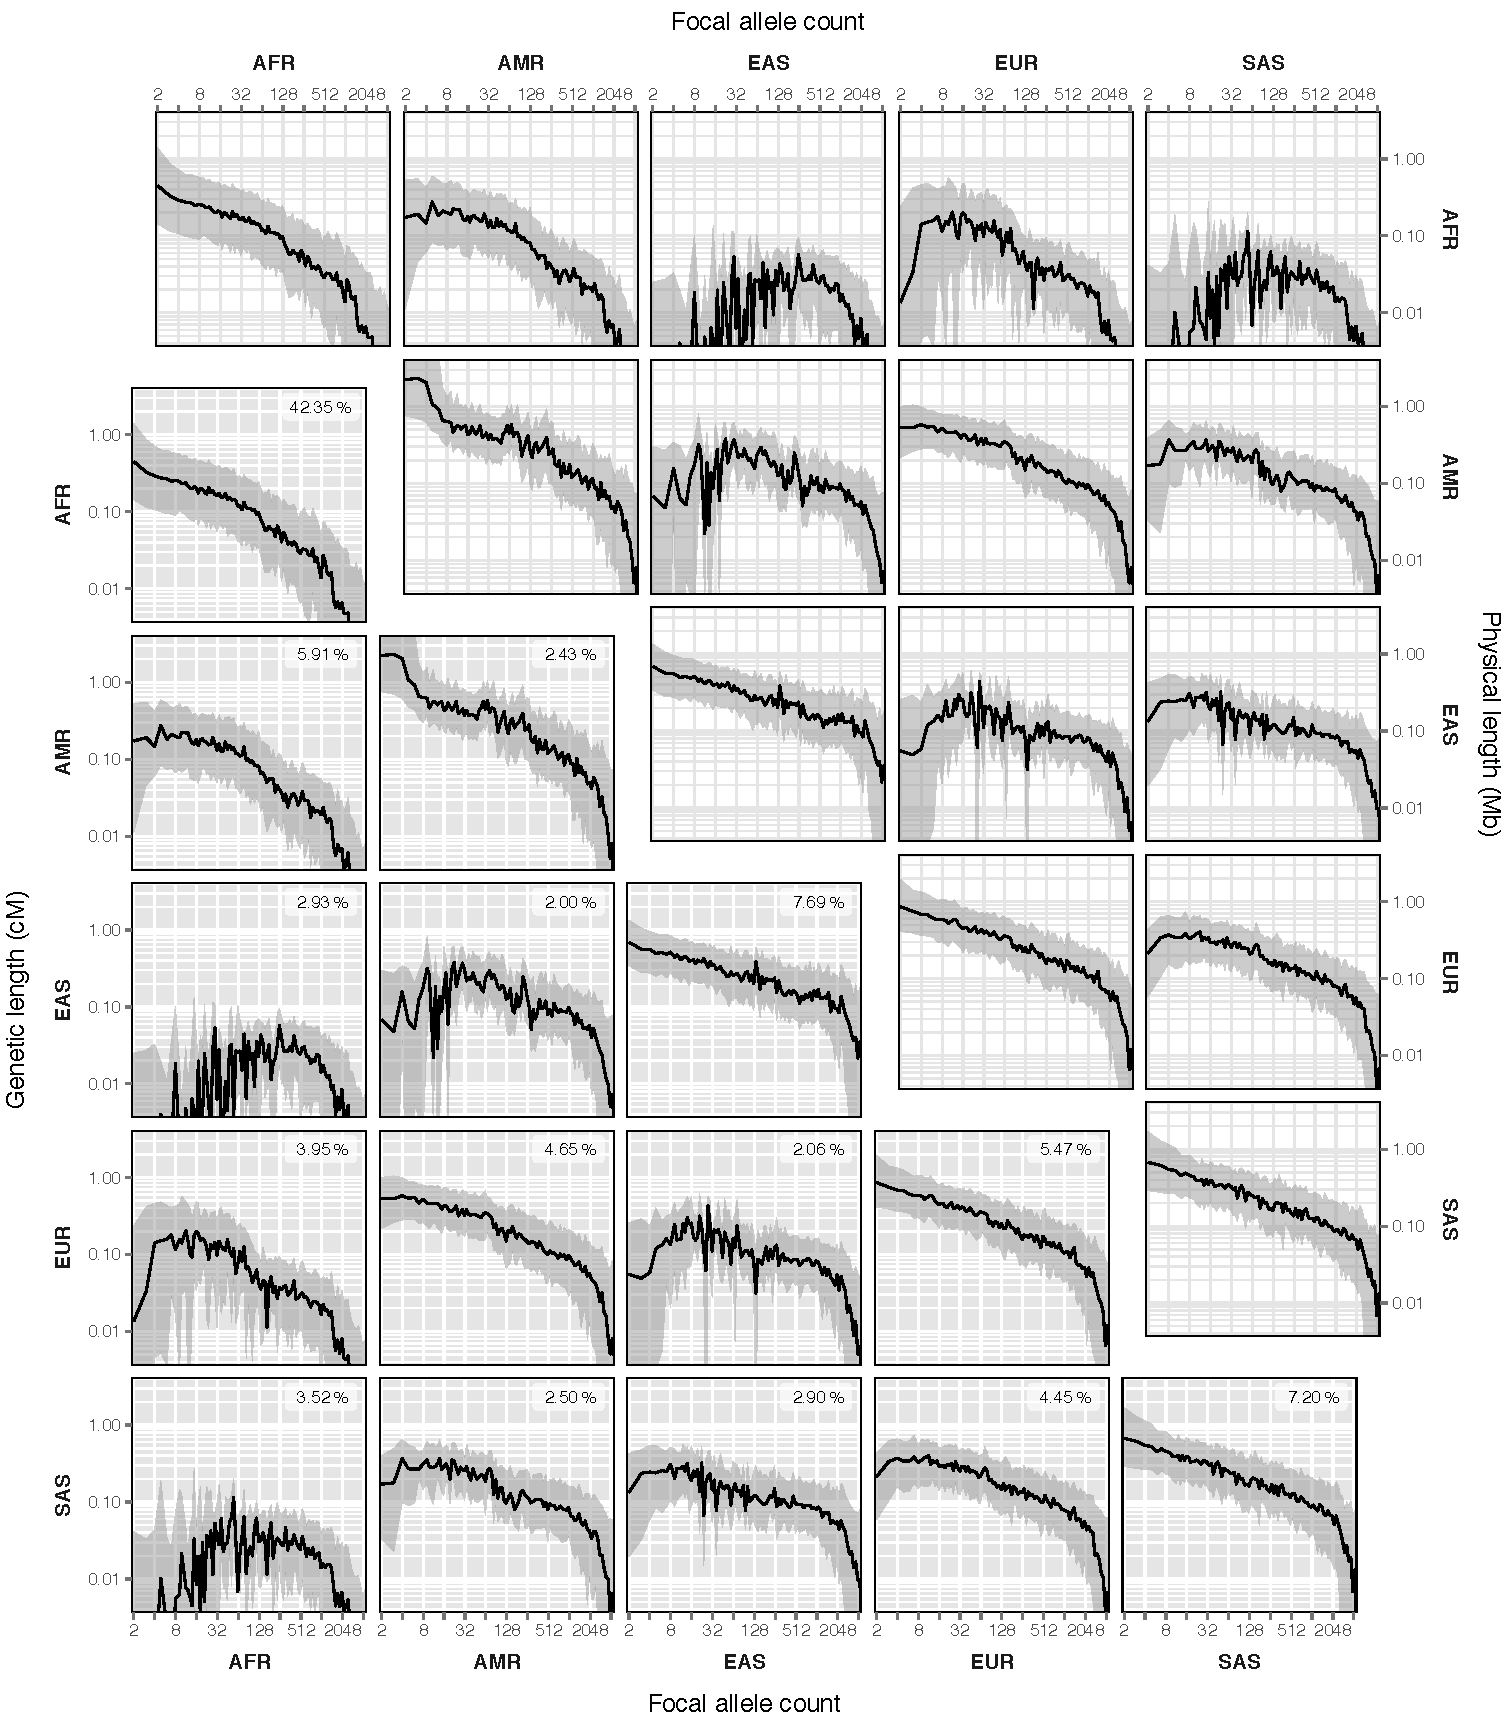
\includegraphics[width=1.1\textwidth]{./img/ch5/1KG20_pop_len_hhmm}%
}
\Caption{Shared haplotype length by population in 1000 Genomes, chromosome~20}%
{Median physical and genetic lengths are shown for haplotype pairs where individuals share a focal allele within the same or between different populations.
Note that the condition of seeing an allele shared between individuals implied that only concordant pairs were considered.
Physical lengths are given in the upper triangle (\emph{white} panels) and genetic lengths in the lower triangle (\emph{grey} panels).
The median (\emph{black} lines) is drawn between the \nth{1} and \nth{3} quartiles, where lengths were binned by focal allele count (log-scale).
The lower triangle also shown the proportions of pairs at which the focal allele was shared within or between populations.}%
{fig:1KG20_pop_len_hhmm}
\end{figure}

%

The average ratio of genetic and physical length was
\SI{1.679922}{\centi\morgan\per\mega\basepair} ($\pm\dec{0.002085}$~SE).
Also, the ratio was similar for discordant pairs;
\SI{1.625225}{\centi\morgan\per\mega\basepair} ($\pm\dec{0.002149}$~SE).
Segment lengths were seen to decrease towards higher focal allele frequencies when alleles were shared within the same population, suggesting an almost linear trend on log-log scale in each population.
However, note that the number of target sites found at higher frequencies was also low.
Segments inferred around rare alleles (\eg \fk{<10}) were relatively long in AFR and AMR, indicating that carrier haplotypes were separated by very recent coalescent events.
In contrast, segments where focal alleles were shared between different populations showed notably shorter lengths at lower frequencies.




%
\subsubsection{Allele age estimated by population}
%

Age was estimated using the relaxed nearest neighbour approach to select discordant pairs, and using the same model parameters per population group.
Note that \Ne is expected to differ across populations, but which may only lead to inappropriate scaling of the population-scaled age estimates per group.
Here, I focused on alleles that were shared only within populations, which retained \n{31906} target sites.
The results for each clock model are shown in \cpref{fig:1KG20_pop_age_hhmm}.

%
%!TEX root = ../../main.tex


\begin{figure}[!htb]
\centering
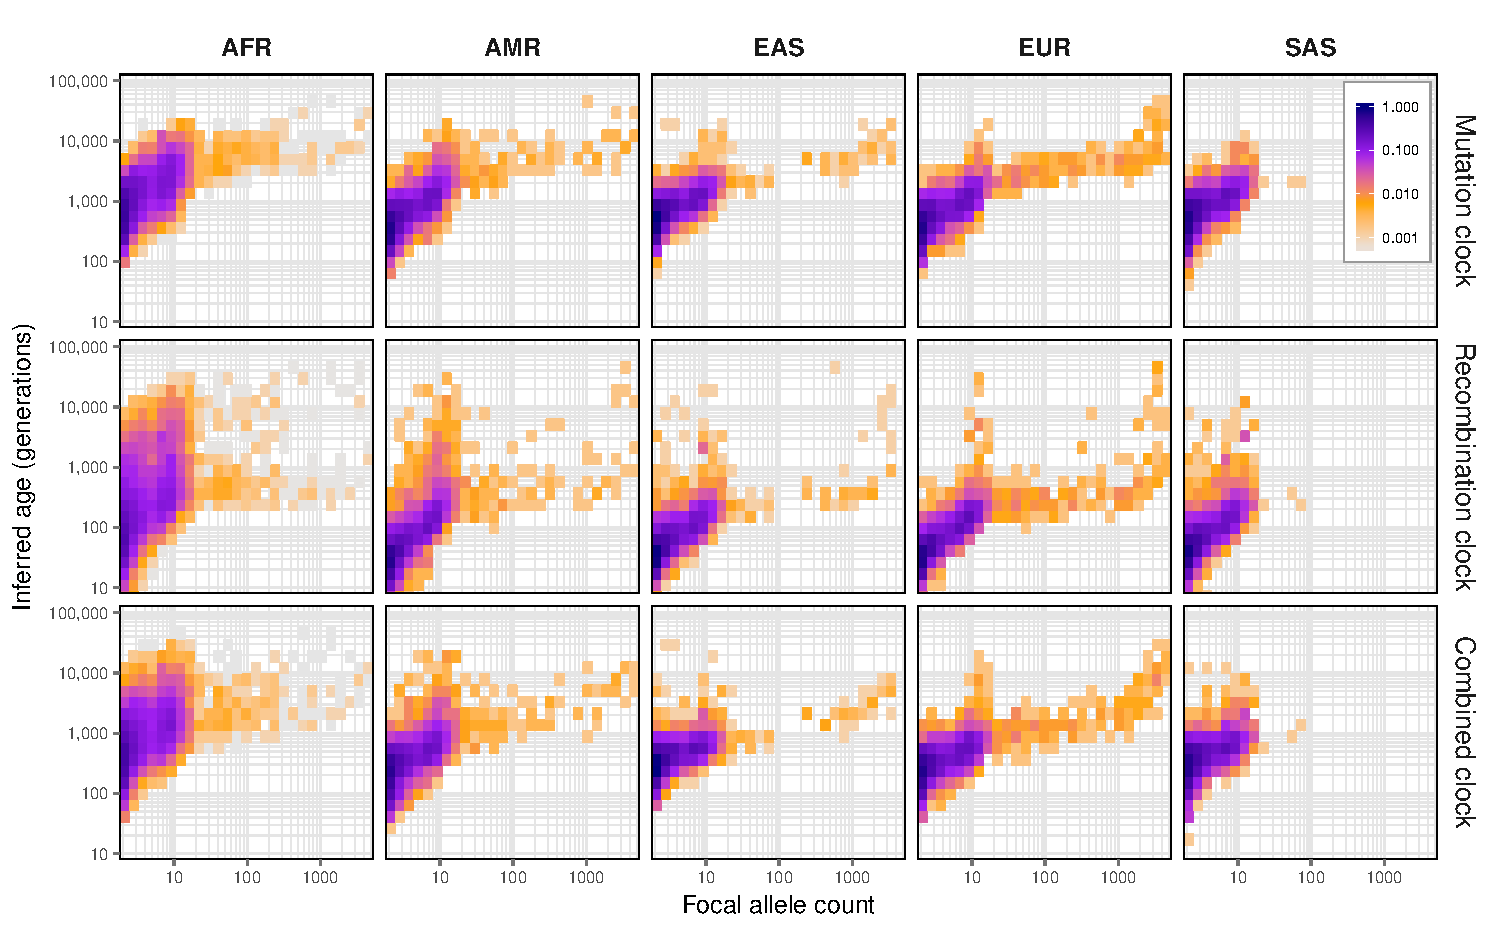
\includegraphics[width=\textwidth]{./img/ch5/1KG20_pop_age_hhmm}
\Caption{Allele age estimated by population in 1000 Genomes, chromosome~20}%
{...}%
{fig:1KG20_pop_age_hhmm}
\end{figure}

%

A general difference was seen between clock models, where age was highest on average in \ClockM, and lowest \ClockR.
But as suggested in previous analyses, \ClockC would be the preferred choice among clock models.
Further, it is not straightforward to compare estimated age distributions between populations, as the number of alleles retained differed substantially among populations and where appropriate scaling of time would be needed to facilitate such comparisons.


%
\subsubsection{Selected allele age profiles}
%

The results presented above produced a holistic picture of the broader distribution of mutational origin at population level.
However, given the amount of work that went into the characterisation of the underlying genealogy at a single locus, such a representation may not capture the relevant aspects that could be explored by focusing on one allele alone.

%
%!TEX root = ../../main.tex


\begin{figure}[p]
\centering
\vspace*{-10pt}
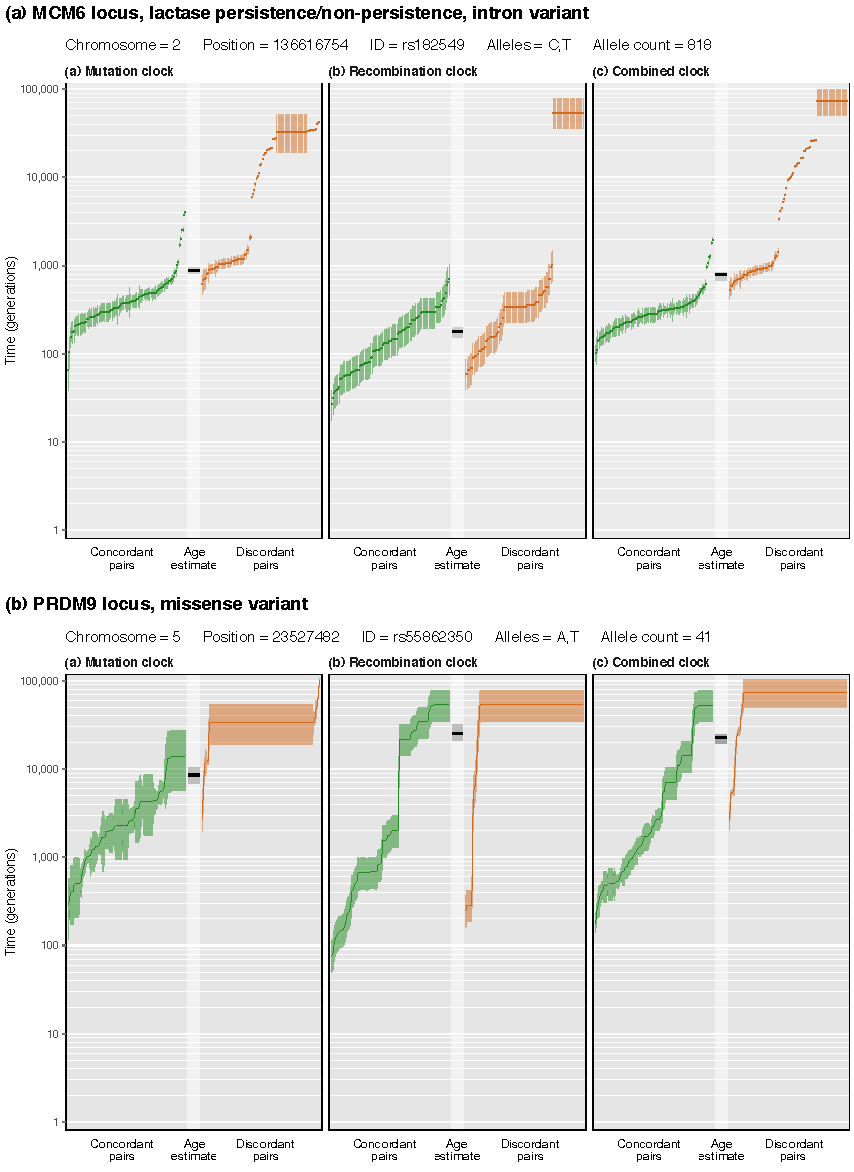
\includegraphics[width=\textwidth]{./img/ch5/1KG20_age_example}
\Caption{Example profiles of estimated allele age in 1000 Genomes, chr.~20}%
{Allele age profiles are shown for \n{2} selected loci in \gls{1kg} data.
Each profile is composed of the \gls{tmrca} posterior distributions inferred for concordant pairs (\emph{left}) and discordant pairs (\emph{right}), which are sorted by their inferred \gls{tmrca}.
The estimated age obtained from the resulting composite posterior distribution is shown in the \emph{middle}.
Each \gls{tmrca} distribution is shown as the median, around which the \nth{1} and \nth{3} quartiles are drawn.
The mode of the composite posterior distribution is shown within a 95\% pseudo-confidence interval.
Time was scaled at $2\Ne$, where ${\Ne=\n{10000}}$.}%
{fig:1KG20_age_example}
\end{figure}

%

\Cpref{fig:1KG20_age_example} shows the \emph{profiles} of the inferred shared haplotype distribution and allele age at \n{2} selected target sites in \gls{1kg}.
Pairs were sorted by \gls{tmrca} to indicate the shape of the underlying genealogy around a given focal site.
Estimated allele age is shown in between the sorted concordant and discordant pairs.

The example shown in \cref{fig:1KG20_age_example}{a} is an intron variant the the MCM6 locus on chromosome~2, which sits approximately \SI{22}{\kilo\basepair} upstream of the LCT gene (encoding the lactase enzyme) and has been associated with lactase persistence in Europeans.
For example, \citet{enattah2002identification} found that the variant occurs in distantly related populations and therefore concluded that it is relatively old.
Research on the LCT gene has indicated signatures of recent positive selection around years ago ${\n{5000}-\n{10000}}$ \citep{bersaglieri2004genetic}.
Here, age estimation suggested that the variant originated at around \n{800} generations ago (according to \ClockC).

A missense variant at the PRDM9 locus in chromosome~5 is shown in \cref{fig:1KG20_age_example}{b}.
Interestingly, the variant is low in frequency in the sample, but its age was estimated to be surprisingly old, and far older in comparison to \cref{fig:1KG20_age_example}{a}.
Note that I also analysed other SNPs at PRDM9 which also indicated an old age and a similar haplotype structure.
However, here, I only attempted to demonstrate one possible application of the methodology, but further research would be needed to arrive at conclusive results for either of the examples provided.




%
% %!TEX root = ../../main.tex


\begin{figure}[!htb]
\centering
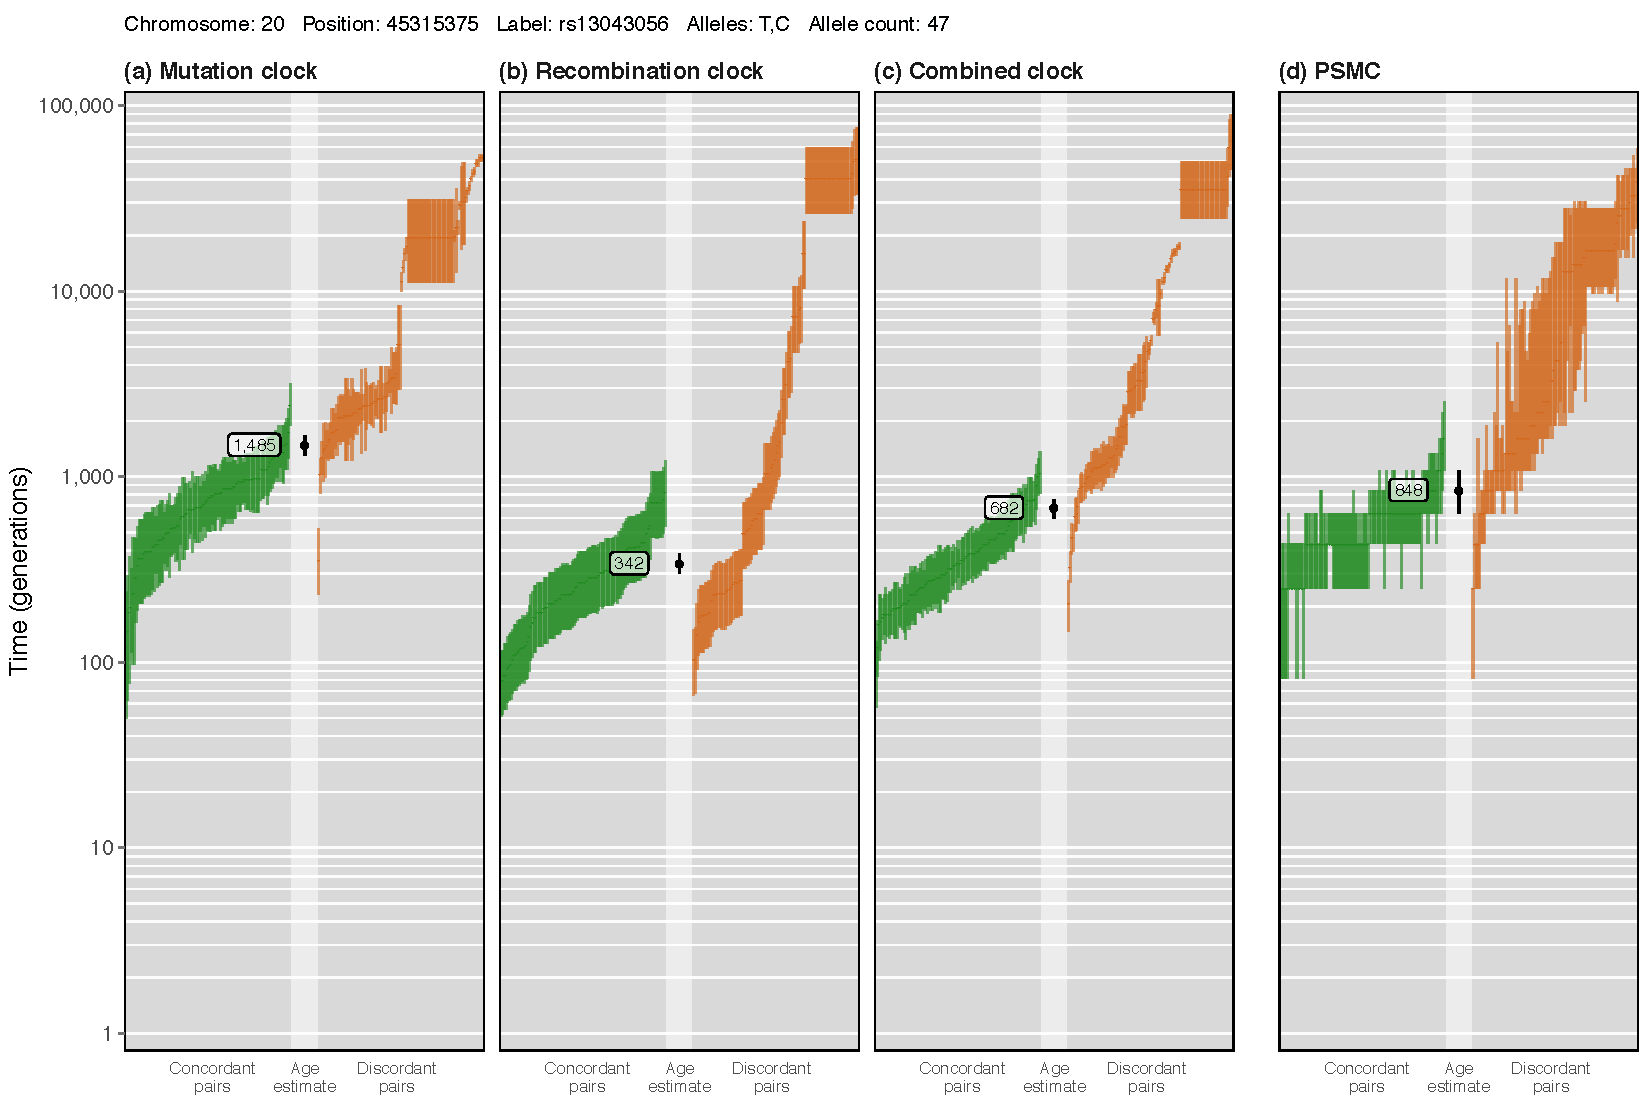
\includegraphics[width=\textwidth]{./img/ch5/1KG20_age_psmc}
\Caption{Example profile for comparison to PSMC in 1000 Genomes, chromosome~20}%
{...}%
{fig:1KG20_age_psmc}
\end{figure}

%


%
\subsection{Discussion}
%

The results in this section provided a general overview of the haplotype structure and allele age distributions that can be expected when the methodology is applied to larger, diverse sample data.
In must be noted that the methods were previously tested on target sites at which no data error was present, but it should be expected that the inclusion of false positive or false negative sites may substantially bias the results.
Although, here, I included sites that were called with high confidence in \gls{1kg}, it was nonetheless possible that allele sharing was flawed at a considerable fraction of sites.

An overview such as presented here can only be limited, because the most interesting observations would arise from looking at particular variant sites; \eg due to effects such as selection, migration, or population stratification.
I presented selected allele age profiles as an example.
In this variant-centric view, ideally, the history of an allele can be observed back in time and followed through different lineages to arrive at the time and place of its origin.
Potential applications include, for example, analyses of alleles previously implicated in disease status, or the identification of previously unnoticed alleles at which indicators of selection are suggested.
%Future research will show to what extent the methodology developed in this thesis is useful.
